% !Mode:: "TeX:UTF-8"
%# -*- coding:utf-8 -*-

%% 南京大学学位论文的示例文档
%% 作者:njuhan: https://github.com/njuHan
%% 源模版repo: https://github.com/njuHan/njuthesis-nju-thesis-template

\documentclass[macfonts,master,twoside]{njuthesis}
%% 审阅模式很重要,命令是下方使用的/blind
%% njuthesis 文档类的可选参数有:
%%   winfonts, linuxfonts, macfonts, adobefonts winfonts b选项使得文档使用Windows 系统提供的字体;linuxfonts 选项使得文档使用Linux 系统提供的字体;macfonts 选项使得文档使用Mac 系统提供的字体;adobefonts 选项使得文档使用Adobe提供的OTF中文字体(需自行下载安转)
%%   phd/master/bachelor 选择博士/硕士/学士论文
%%   twoside 或 oneside 指定排版的文档为双面打印或单面打印格式(twoside会使得chapter 章节从奇数页开始,即纸张的正面开始,因此会出现一些空白的页面)
%%   nobackinfo 取消封二页导师签名信息。注意,按照南大的规定,是需要签名页的。



%%%%%%%%%%%%%%%%%%%%%%%%%%%%%%%%%%%%%%%%%%%%%%%%%%%%%%%%%%%%%%%%%%%%%%%%%%%%%%%
% set up labelformat and labelsep for subfigure 详见: http://www.latexstudio.net/archives/8652.html
\captionsetup[subfigure]{labelformat=simple, labelsep=space}

%%%%%%%%%%%%%%%%%%%%%%%%%%%%%%%%%%%%%%%%%%%%%%%%%%%%%%%%%%%%%%%%%%%%%%%%%%%%%%%
% 设置《国家图书馆封面》的内容,仅博士论文才需要填写

% 设置论文按照《中国图书资料分类法》的分类编号
%\classification{0175.2}
% 设置论文按照《国际十进分类法UDC》的分类编号
% 该编号可在下述网址查询:http://www.udcc.org/udcsummary/php/index.php?lang=chi
%\udc{004.72}
% 国家图书馆封面上的论文标题第一行,不可换行。此属性可选,默认值为通过\title设置的标题。
%\nlctitlea{论文标题第一行}
% 国家图书馆封面上的论文标题第二行,不可换行。此属性可选,默认值为空白。
%\nlctitleb{论文标题第二行}
% 国家图书馆封面上的论文标题第三行,不可换行。此属性可选,默认值为空白。
%\nlctitlec{}
% 导师的单位名称及地址
%\supervisorinfo{南京大学计算机科学与技术系~~南京市汉口路22号~~210093}
% 答辩委员会主席
%\chairman{张三丰~~教授}
% 第一位评阅人
%\reviewera{阳顶天~~教授}
% 第二位评阅人
%\reviewerb{张无忌~~副教授}
% 第三位评阅人
%\reviewerc{黄裳~~教授}
% 第四位评阅人
%\reviewerd{郭靖~~研究员}


%%%%%%%%%%%%%%%%%%%%%%%%%%%%%%%%%%%%%%%%%%%%%%%%%%%%%%%%%%%%%%%%%%%%%%%%%%%%%%%
% 设置论文的中文封面


% % 单行论文标题,不可换行
\title{}
\titlea{面向Hyperledger Fabric的}
\titleb{区块链云化框架的研究与实现}

% 如果论文标题过长,可以分两行,第一行用\titlea{}定义,第二行用\titleb{}定义,
% 使用以下3行:
%\title{} %用于覆盖单行标题内容为空
%\titlea{长标题第一行}  %第一行标题写这里
%\titleb{长标题第二行用于长标题换行} %第二行标题写这里
% 注意: \title 不能都注释,它用于控制标题选择双行还是单行。\title{}如果内容为空,则编译\titlea{},titleb{}双行标题,否则编译单行标题


% 论文作者姓名
\author{张富利}
% 论文作者联系电话
\telphone{18851751795}
% 论文作者电子邮件地址
\email{MG1932016@smail.nju.edu.cn}
% 论文作者学生证号
\studentnum{MG1932016}
% 论文作者入学年份(年级)
\grade{2019}
% 论文作者毕业年份(届), 出版授权书的学位年度
\graduateyear{2022}
% 导师姓名职称
\supervisor{张贺~~教授}
% 导师的联系电话
\supervisortelphone{}
% 论文作者的学科与专业方向
\major{软件工程}
% 论文作者的研究方向
\researchfield{DevOps、区块链}
% 论文作者所在院系的中文名称
\department{软件学院}
% 论文作者所在学校或机构的名称。此属性可选,默认值为``南京大学''。
\institute{南京大学}
% 论文的提交日期,需设置年、月、日。
\submitdate{xxxx年 xx 月 xx 日}
% 论文的答辩日期,需设置年、月、日。
\defenddate{xxxx年 xx 月 xx 日}
% 论文的定稿日期,需设置年、月、日。
% 此属性可选,若注释\date{},则默认值为最后一次编译时的日期,精确到日。
% \date{2019年5月20日}

%%%%%%%%%%%%%%%%%%%%%%%%%%%%%%%%%%%%%%%%%%%%%%%%%%%%%%%%%%%%%%%%%%%%%%%%%%%%%%%
% 设置论文的英文封面

% 论文的英文标题,不可换行
\englishtitle{Research and Implementation of A
Blockchain Cloudification Framework for Hyperledger Fabric}
\englishabstracttitlea{Research and Implementation of}
\englishabstracttitleb{A Blockchain Cloudification Framework for Hyperledger Fabric}
% 论文作者姓名的拼音
\englishauthor{Fuli Zhang}
% 导师姓名职称的英文
\englishsupervisor{Professor~~He Zhang}
% 论文作者学科与专业的英文名
\englishmajor{Software Engineering}
% 论文作者所在院系的英文名称
\englishdepartment{Software Institute}
% 论文作者所在学校或机构的英文名称。此属性可选,默认值为``Nanjing University''。
\englishinstitute{Nanjing University}
% 论文完成日期的英文形式,它将出现在英文封面下方。需设置年、月、日。日期格式使用美国的日期
% 格式,即``Month day, year'',其中``Month''为月份的英文名全称,首字母大写;``day''为
% 该月中日期的阿拉伯数字表示;``year''为年份的四位阿拉伯数字表示。
% 此属性可选,若注释掉\englishdate{},则默认值为最后一次编译时的日期。
% \englishdate{May 20, 2019}

%%%%%%%%%%%%%%%%%%%%%%%%%%%%%%%%%%%%%%%%%%%%%%%%%%%%%%%%%%%%%%%%%%%%%%%%%%%%%%%
% 设置论文的中文摘要

% 设置中文摘要页面的论文标题及副标题的第一行。
% 此属性可选,其默认值为使用|\title|命令所设置的论文标题
\abstracttitlea{面向Hyperledger Fabric的}
% 设置中文摘要页面的论文标题及副标题的第二行。
% 此属性可选,其默认值为空白
\abstracttitleb{ \qquad \qquad \qquad 区块链云化框架的研究与实现}

%%%%%%%%%%%%%%%%%%%%%%%%%%%%%%%%%%%%%%%%%%%%%%%%%%%%%%%%%%%%%%%%%%%%%%%%%%%%%%%
% 设置论文的英文摘要

% 设置英文摘要页面的论文标题及副标题的第一行。
% 此属性可选,其默认值为使用|\englishtitle|命令所设置的论文标题
%\englishabstracttitlea{englishabstracttitlea}
% 设置英文摘要页面的论文标题及副标题的第二行。
% 此属性可选,其默认值为空白
%\englishabstracttitleb{nglishabstracttitleb}

%%%%%%%%%%%%%%%%%%%%%%%%%%%%%%%%%%%%%%%%%%%%%%%%%%%%%%%%%%%%%%%%%%%%%%%%%%%%%%
%% 盲审命令,空白字段设置请看 .cls文件 \newcommand*{\blind}
%% 此外,请按照盲审要求自行去掉个人简历、致谢等页面中的个人信息
%%**********************!!!非常重要的盲审命令,送审前必选!!!****************
\blind
%%**********************!!!非常重要的盲审命令,送审前必选!!!****************

%%%%%%%%%%%%%%%%%%%%%%%%%%%%%%%%%%%%%%%%%%%%%%%%%%%%%%%%%%%%%%%%%%%%%%%%%%%%%%%
\begin{document}

%%%%%%%%%%%%%%%%%%%%%%%%%%%%%%%%%%%%%%%%%%%%%%%%%%%%%%%%%%%%%%%%%%%%%%%%%%%%%%%

% 制作国家图书馆封面(博士学位论文才需要)
% \makenlctitle
% 制作中文封面
\maketitle
% 制作英文封面
\makeenglishtitle

%%%%%%%%%%%%%%%%%%%%%%%%%%%%%%%%%%%%%%%%%%%%%%%%%%%%%%%%%%%%%%%%%%%%%%%%%%%%%%%
% 开始前言部分
\frontmatter

\begin{abstract}
  区块链具有去中心化、不可篡改的特性, 被誉为新型生产关系。区块链的发展为传统领域带来了巨大变革, 去中心化应用逐步从理论论证阶段转变为工程化实践阶段。BaaS作为一种构建、管理、托管和运维区块链网络及去中心化应用的云服务平台, 在一定程度上降低了去中心化应用落地的门槛。

  然而, 当前区块链的发展依旧存在诸多问题。首先, 区块链的基础商业应用工具不完善。BaaS平台尚在初级阶段, 研发投入巨大。市场上BaaS平台被头部云厂商垄断, 行业马太效应明显。不同BaaS平台缺乏统一的顶层规划, 形成数据孤岛。其次, BaaS平台利用云能力赋能区块链乏力。BaaS平台仅提供一种基于开源区块链平台的自动部署方案, 未深入区块链与云基础设施底层。因此, BaaS平台无法挖掘云原生技术的潜力, 提供安全、可扩展、高可用的区块链服务。最后, 智能合约缺少标准的开发运维流程, 缺少促进去中心化应用价值交付的有效手段。
  
  因此, 针对上述挑战, 本文综合考虑区块链网络节点以及智能合约的开发运维两个维度, 提出了面向Hyperledger Fabric的区块链云化框架。首先, 本文通过快速评审的方法, 调研学术界如何利用Kubernetes Operator赋能传统领域, 最终整理出11条赋能策略集。本文结合区块链云化的原则和区块链本身特性筛选并获得区块链网络节点云化实施方案。其次, 本文对比了智能合约与微服务在设计原则上的相似性, 进行了智能合约微服务化改造, 并提出了智能合约微服务化开发运维流程。然后, 基于区块链网络节点云化实施方案以及智能合约微服务化开发运维流程, 本文设计实现了面向Hyperledger Fabric的区块链云化框架及其原型工具。

  本文对框架及原型工具进行了基础功能自证、成熟度衡量、对比分析三维度的测试与评估。在基础功能自证方面, 通过典型案例对原型工具进行了功能可行性测试, 利用SAAM架构评估方法验证质量属性。在成熟度衡量方面, 本文结合Kubernetes Operator五层成熟度模型进行了定性评估。在对比分析方面, 本文与官方BaaS平台Cello对比进行了定量评估。结果表明, 本文提出的框架及原型平台在兼容BaaS基本功能前提下充分利用云的特性提升了Hyperledger Fabric网络的可移植性、可靠性、易用性、可扩展性以及安全性, 其基本满足五层成熟度的能力要求并且拥有更优的网络部署时间和链码交付效率。

	% 同时应该注意到,空白页是故意留白,以便章节开头能够出现在偶数页。
	% 中文关键词。关键词之间用中文全角分号隔开,末尾无标点符号。
	\keywords{区块链, 云原生, BaaS, Kubernetes Operator}
\end{abstract}

%%%%%%%%%%%%%%%%%%%%%%%%%%%%%%%%%%%%%%%%%%%%%%%%%%%%%%%%%%%%%%%%%%%%%%%%%%%%%%%
% 论文的英文摘要
\begin{englishabstract}
  Blockchain has the advantages of decentralization and immutability. It is known as the next production relationship. The development of blockchain has brought great changes to the traditional field, and decentralized applications have gradually shifted from the theoretical demonstration stage to the engineering practice stage. As a cloud service platform for building, managing, hosting and operating blockchain networks and decentralized applications, BaaS greatly reduces the threshold for implementation of decentralized applications.

  However, there are still many problems in the current development of blockchain-based systems. First, the commercial tools of blockchain are not perfect. The BaaS platform is still in its infancy, with huge R\&D investment. In the market, the BaaS platform is monopolized by the top cloud manufacturers, and the Matthew effect of the industry is obvious. Different BaaS platforms lack unified top-level planning, resulting in isolated islands of data. Secondly, the BaaS platform is weak in empowering the blockchain with cloud capabilities. The BaaS platform only provides an automatic deployment solution based on the open source blockchain platform, without going deep into the principles of the blockchain and cloud infrastructure. Therefore, the BaaS platform cannot tap the potential of cloud-native technology to provide secure, scalable and highly available blockchain services. Finally, smart contracts lack standard development and operation processes, and lack effective means to promote the value delivery of decentralized applications.

  Therefore, in response to the problems, this thesis proposes a cloudification framework for blockchain based on Hyperledger Fabric by comprehensively considering the blockchain network nodes and smart contracts. Firstly, this thesis surveys how academia uses Kubernetes Operator to empower traditional fields through a rapid review method and sorts out eleven enabling strategy sets. The blockchain nodes cloudification plan is obtained by filtering the principles of blockchain cloudification and the characteristics of blockchain itself. Secondly, this thesis compares the similarities between smart contract and microservice in design principles, carries out the refactor of smart contract into microservice, and proposes the process of developing and operating microservices for smart contracts. Then, based on the cloud implementation plan of blockchain network nodes and the process of smart contract microservices, this thesis designs and implements the blockchain cloudification framework and its prototype platform for Hyperledger Fabric.

  In this thesis, the framework and prototype tool are tested and evaluated in three dimensions: self-validation of basic functions, maturity measurement, and comparative analysis. In terms of self-certification of basic functions, the functional feasibility test of the prototype tool is carried out through a typical case analysis, and the quality attribute is verified by the SAAM architecture evaluation method. In terms of maturity measurement, this thesis conducts a qualitative evaluation based on the five maturity levels of Kubernetes Operator. In terms of comparative analysis, this thesis conducts a quantitative evaluation compared with the official BaaS platform Cello.The test and evaluation results show that the framework and prototype tool can make full use of the characteristics of the cloud to improve the portability, reliability, usability, scalability, and security of Hyperledger Fabric network. The prototype tool basically meets the requirements of five maturity levels and has better results than Cello in terms of deployment time and delivery efficiency.
  
  \englishkeywords{Blockchain, Cloud Native, BaaS, Kubernetes Operator}
\end{englishabstract}


%%%%%%%%%%%%%%%%%%%%%%%%%%%%%%%%%%%%%%%%%%%%%%%%%%%%%%%%%%%%%%%%%%%%%%%%%%%%%%%
% 论文的前言,应放在目录之前,中英文摘要之后,一般不需要
%
%\begin{preface}
%
%在过去的40年中,手写中文文本领域识别(HCTR)取得了很大的进展[1,2]。
%
%\vspace{1cm}
%\begin{flushright}
%饶安逸\\
%2018年5月15日于南大仙林
%\end{flushright}
%
%\end{preface}

%%%%%%%%%%%%%%%%%%%%%%%%%%%%%%%%%%%%%%%%%%%%%%%%%%%%%%%%%%%%%%%%%%%%%%%%%%%%%%%
% 生成论文目录
\tableofcontents

%%%%%%%%%%%%%%%%%%%%%%%%%%%%%%%%%%%%%%%%%%%%%%%%%%%%%%%%%%%%%%%%%%%%%%%%%%%%%%%
% 生成插图清单。如无需插图清单则可注释掉下述语句。
\listoffigures

%%%%%%%%%%%%%%%%%%%%%%%%%%%%%%%%%%%%%%%%%%%%%%%%%%%%%%%%%%%%%%%%%%%%%%%%%%%%%%%
% 生成附表清单。如无需附表清单则可注释掉下述语句。
\listoftables

%%%%%%%%%%%%%%%%%%%%%%%%%%%%%%%%%%%%%%%%%%%%%%%%%%%%%%%%%%%%%%%%%%%%%%%%%%%%%%%
% 开始正文部分
\mainmatter

%%%%%%%%%%%%%%%%%%%%%%%%%%%%%%%%%%%%%%%%%%%%%%%%%%%%%%%%%%%%%%%%%%%%%%%%%%%%%%%
% 学位论文的正文应以《绪论》作为第一章,本模板是按照自身功能模块组织的,并非论文中的章节安排


\chapter{绪论}

\section{研究背景及意义}

区块链(Blockchain)是一种按照时间顺序将数据区块以链条的方式组成的特定数据结构,被视为一个分布式的共享账本和数据库。它能够使用户无需相互信任与可信第三方的条件下完成可信的价值传输\cite{SurveyofEnterpriseBlockchains}。作为区块链2.0 的以太坊\footnotemark[1]\footnotetext[1]{\href{http://github.com/ethereum/wiki/wiki/White-Paper/}{以太坊白皮书}}重新将智能合约描述为图灵完备的、部署于区块链网络中合同条款代码。这意味着传统的合同条款可以进入实体计算机中,且在区块链网络去中心化、不可伪造、不可篡改的特性下严格执行。区块链推进了人与企业之间和线上与线下之间的全方面互联,其被成为下一代的新型生产关系。随着区块链的快速发展, 智能合约极大地丰富和扩展了区块链应用场景。它们为供应链、金融等传统领域带来重大变革, 已经快速渗入到人们生活的方方面面。

与此同时, 云原生(Cloud native)作为一种基于云的基础之上的软件架构思想,以及基于云进行软件开发实践的一组方法论。因其弹性和分布式的优势成为当今流行的软件服务模式。云原生技术有利于各组织在公有云、私有云和混合云等新型动态环境中, 构建和运行可弹性扩展的应用, 借助平台的全面自动化能力, 跨多云构建微服务, 持续交付部署业务生产系统。

{\footnotesize
\begin{longtable}[h]{m{100pt} m{50pt} m{50pt} m{50pt} m{50pt}}
    \caption[主要公有云的BaaS平台]{主要公有云的BaaS平台} \label{major_BaaS_platforms} \\
        \toprule  
        \textbf{BaaS平台}&\textbf{Ethereum}&\textbf{Quorum}&\textbf{Corda}&\textbf{Fabric}\\
        \hline
        
        AWS&Y&Y&Y&Y\\

        Azure&Y&Y&Y&Y\\

        IBM& & & &Y\\

        阿里云区块链服务&Y& & &Y\\

        腾讯云区块链服务TBaaS& & & &Y\\

        华为云区块链服务BCS& & & &Y\\
        \bottomrule
    \end{longtable}
}

区块链即服务(Blockchain as a Service, 简称BaaS)则是基于云原生技术体系的一种构建、管理、托管和运维区块链网络及其应用的云服务平台\cite{onik2019performance}。BaaS支持将任何企业级区块链实施到云环境,而无需任何IT专业知识。这大大降低了区块链技术的使用门槛, 是促使区块链技术更广泛、更深入地渗透到各个行业和企业的催化剂, 其市值预计从2018年的6.23亿美元猛增2023年的150亿美元\footnotemark[1]\footnotetext[1]{\href{https://www.reportbuyer.com/product/5486837/global-blockchain-as-a-service-market.html}{Global Blockchain-as-a-Service Market 2018-2022}}。其中, 云厂商提供了大多数的BaaS平台\cite{KuernetesbasedFabricChaincodeManagementAndHihgAvailabilityTechnology}, 如表\ref{major_BaaS_platforms}所示, 其底层区块链支撑技术大多数选择IBM开源的跨企业级联盟链Hyperledger Fabric, 这也是本文选择Hyperledger Fabric的原因。


% 挑战
BaaS基于云的弹性可伸缩的能力屏蔽了底层区块链技术, 为上层去中心化应用的开发运维人员提供便捷的构建区块链网络等功能。然而, “Each coin has two sides”, 当前BaaS平台的发展尤其是底层的区块链基础设施的建设依旧存在诸多挑战。

首先, 基础商业化应用工具并不完善\footnotemark[2]\footnotetext[2]{\href{http://www.caict.ac.cn/kxyj/qwfb/ztbg/202107/P020210726503897354430.pdf}{区块链基础设施研究报告(2021年)}}。BaaS平台发展还处于初级阶段, 商业运行模式仍处在探索阶段。由于BaaS平台研发投入大, 目前市场上存在如AWS、IBM、阿里云区块链服务等多种BaaS平台解决方案, 这些BaaS平台计费高昂\footnotemark[3]\footnotetext[3]{\href{https://help.aliyun.com/document_detail/107710.html?spm=5176.14107623.commonbuy2container.1.59523b20xmyuNf}{阿里云区块链服务BaaS规格与定价}}并且与其他云服务捆绑销售。传统的企业业务或已存在稳定合作的云服务商, 使用不同云服务商的合作伙伴就需要跨云部署, 由于缺乏统一的顶层规划, 各云厂商的BaaS导致不同应用底层异构形成技术、信息孤岛, 存在不可复用的跨解决方案的资源和工具, 这导致了基于多云的网络\cite{DBLP:conf/coins/GerritsKKFV21}, 给跨云部署带来了诸多问题。同时, BaaS平台几乎都由互联网云服务巨头企业把控, 可用性限制通常会迫使其他企业为来自各种云提供商的基础设施即服务(Infrastructure as a Service, 简称IaaS)付费, 最终行业马太效应明显\cite{KuernetesbasedFabricChaincodeManagementAndHihgAvailabilityTechnology}。

其次, BaaS平台利用云能力对区块链基础设施赋能乏力。作为一种广泛部署的技术, 云计算是实施区块链技术的合适目标。然而, 区块链与云原生两种技术都相对不成熟, 但两者的集成可能会在技术方面产生新的复杂性\cite{onik2019performance}。行业缺少既定的标准或最佳实践范例, 各云厂商的BaaS解决方案基本都采取已有的开源解决方案, 业务同质化严重。他们 仅提供一种基于开源区块链平台的自动部署管理方案, 未深入到区块链与云基础设施的底层, 问题仍然在于如何使区块链和云兼容\cite{gai2020blockchain}, 区块链服务比常规云服务更复杂, 有许多未解决的问题需要回答。自动化脚本部署并不是有效的云化方式, 浪费了云原生技术的潜力。例如除区块链网络自动部署外, 在数据存储备份及可扩展性方面, 传统自动化部署方案无法利用云的弹性伸缩能力性且随着交易数量的增加, 区块数据最终会占满磁盘空间, 出现存储膨胀问题。区块链的数据可扩展性受到了的限制, 需要结合云的能力寻找数据备份、升级及可扩展性的方法。区块链如何和云原生快速深度结合, 利用原生伸缩性、可移植性和高可用性价值来提供“高质量”的区块链服务, 是当前仍然遗留的挑战。

% 意义、愿景
针对上述问题, 本文选择面向联盟链场景开源框架Hyperledger Fabric和Kubernetes提出了一种基于Hyperledger Fabric的区块链云化框架, 具体工作如图\ref{framework_tool}所示。该框架通过对Fabric网络中的Ca、Orderer、Peer组件进行抽象适配并利用Kubernetes Operator对其进行完整生命周期管理。本框架利用原生Kubernetes安全性、可扩展性等机制使用户通过专家提供的领域知识对Fabric网络获得类似云的自我管理。此外, 本文还实现了基于区块链云化框架的原型工具, 支持更简单、更原生的管理Fabric网络。

\begin{figure}[h] %figure环境,h默认参数是可以浮动,不是固定在当前位置。如果要不浮动,你就可以使用大写float宏包的H参数,固定图片在当前位置,禁止浮动。
    \centering %使图片居中显示
    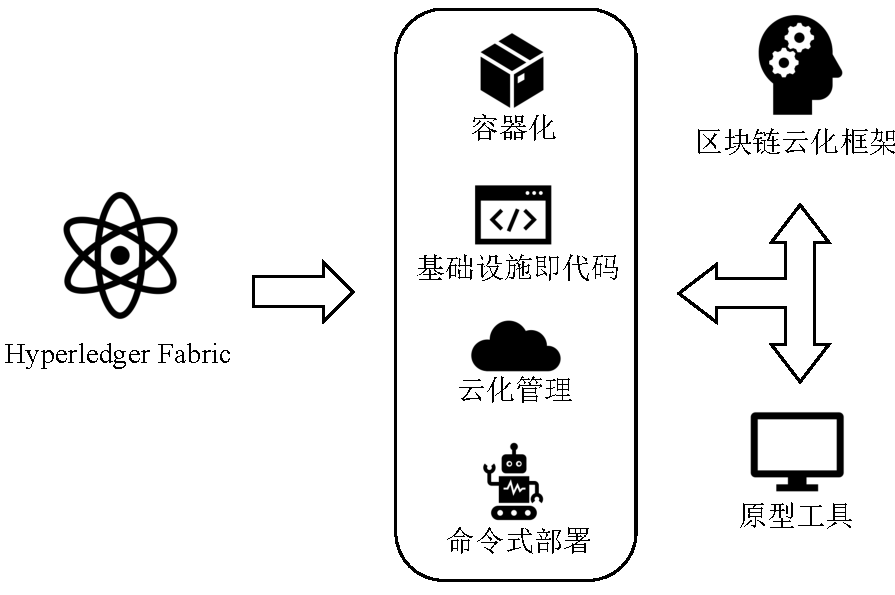
\includegraphics[width=0.7\textwidth]{FIGs/chapter1/framework_tool.pdf} %中括号中的参数是设置图片充满文档的大小,你也可以使用小数来缩小图片的尺寸。
    \caption{区块链云化框架及其原型工具} %caption是用来给图片加上图题的
    \label{framework_tool} %这是添加标签,方便在文章中引用图片。
\end{figure}%figure环境

\section{研究现状}

由于区块链智能合约的无法删除、修改、历史可追溯、去中心化、严格执行等特点, 越来越多的研究人员想挖掘区块链的潜能, 将区块链的能力应用到各种应用场景。McCorry等人\cite{mccorry2017smart}将区块链应用在电子投票领域, 实现了一个基于以太坊的去中心化互联网公开投票协议,公开投票网络是一种自助协议, 每个选民都控制着自己投票的隐私, 只有在所有人都参与的情况下才会被破坏, 这是第一个实现的不依赖任何可信的权威机构来计数和保护选民隐私的去中心化应用。Chang和Chen\cite{chang2020blockchain}在供应链领域进行了系统文献综述,表明传统的供应链活动涉及多个中介、信任和性能问题,利用区块链的潜力可以更好地扰乱供应链运作性能、分布式治理和过程自动化。Zhang和Wen\cite{zhang2017iot}提出了一种物联网电子商务模型,旨在重新设计传统电子商务模型中的许多元素,并借助区块链和智能合约技术在物联网上实现智能财产和付费数据的交易。Leka等人\cite{leka2019systematic}相信区块链技术将是下一个技术革命,同时表明区块链研究现阶段在物联网\cite{christidis2016blockchains}、医疗、教育、政府各个领域都有涉及。

目前, 去中心化应用逐步从概念验证阶段转变为工程化、商业化阶段。由于区块链的复杂性给网络的构建以及智能合约的部署、运维工作带来了严重的时间成本。在去中心化应用价值交付过程中, 存在对于区块链底层技术的易用性、部署效率、安全性等多方面的挑战。研究人员在区块链基础设施与云原生结合方面都开始了一定的探索, 除了利用区块链的特性提升云的能力外\cite{DBLP:journals/comcom/XieZZWH21}\cite{DBLP:conf/smartcloud/SunWY20}\cite{8457813}, 研究人员也都期望利用云的特性自动化地构建出易于弹性扩展、高可用的区块链平台。

% 学术
% 应用场景 BaaS平台往云上迁移
在学术研究方面, 研究人员在探究如何有效利用云平台来部署区块链平台。Gerrits等人\cite{DBLP:conf/coins/GerritsKKFV21}在Kubernetes中部署了分布式账本Hyperledger Sawtooth\footnotemark[1]\footnotetext[1]{\href{https://github.com/hyperledger/sawtooth-core}{Hyperledger Sawtooth github地址}}, 并运行了一个用例。他们旨在探讨该用例在真实场景云部署中的可行性和可扩展性。Liang等人\cite{liangeduchain}针对教育领域数据共享和信息欺骗的问题构建了一个高可用的教育联盟区块链平台, 并实现了基于Kubernetes的Fabric部署, 实现了将链码纳入Kubernetes环境管理的目标。然而, Wan等人\cite{wan2018novel}指出当前主流的BaaS提供商通常采用API进行用户访问, 或者简单地将区块链应用迁移到云, 这会侵蚀不可信的机制并带来锁定风险。他们随后提出了一种新的服务范式来克服现有BaaS的局限性。基于Hyperledger的实施表明, 该范式可以缓解当前BaaS对区块链特征的侵蚀。在云原生底层基础设施方面研究人员关注与区块链结合的Kubernetes调度问题。才\cite{caili2018}在Kubernetes上面对PBFT和区块链的本身特性提出了静态调度和自适应算法。Shi等人\cite{9582270}为了解决云端现实PoS区块链工作负载的高效调度问题, 首次在云计算中设计和实现了基于Kubernetes的解决PoS区块链应用程序迁移成本的系统, 最大限度地减少了使用的Kubernetes工作节点数量以降低总体费用,而且还提出了一种高性能的Kubernetes调度方案HPKS以最大限度地利用工作节点进行在线pod管理。

% 工业界
相比于学术研究, 工业领域的探索更加注重自动化实践。Hyperledger Cello\footnotemark[1]\footnotetext[1]{\href{https://github.com/hyperledger/cello}{Hyperledger Cello github地址}}支持在多种底层基础设施上从头快速构建BaaS平台, 提供管理区块链网络的生命周期、自定义区块链网络配置等功能帮助人们以更高效的方式使用和管理区块链。Hyperledger Cello当前阶段重点关注在Docker安装, 对于Kubernetes支持方面的仍处在相对初级阶段, 配置项简单灵活性不足且老旧。Blockchain Automation Framework\footnotemark[2]\footnotetext[2]{\href{https://github.com/nikoturin/blockchain-automation-framework}{Blockchain Automation Framework github地址}}提供了一个自动化框架, 利用Ansible\footnotemark[3]\footnotetext[3]{\href{https://github.com/ansible/ansible}{Ansible github地址}}以及Helm\footnotemark[4]\footnotetext[4]{\href{https://github.com/helm/helm}{Helm github地址}}快速地、一致地将生产就绪的分布式账本技术(Distributed ledger technology, 简称DLT)平台部署到云基础设施。虽然, Blockchain Automation Framework提供了一个自动化框架将区块链平台部署于Kubernetes, 但本质上还是描述为一个需要希望远程主机执行命令的方案,或者一组IT程序运行的命令集合。这大大提升了自动化程度,但其远没有发挥Kubernetes的潜力。

% 总结
尽管学术界以及工业界目前已有一些关于区块链云化的探索与研究, 研究重点多为如何自动化地将区块链平台向云上迁移, 研究缺少构建支持云和区块链一体化的有效服务模型\cite{9582270}。

与此同时, 一部分研究利用Kubernetes operator方法将云底层的效率、灵活性等多方面优势拓展到多种领域。Kubernetes operator是将领域知识集成到Kubernetes API编排过程中的最新方法\cite{henning2021reproducible}。Huang等人\cite{huang2021fly}提出了一个轻量级的遥感大数据处理云原生框架。该框架利用Kubernetes operator融合Spark, 自动化配置Spark参数, 提升并行遥感图像融合算法的效率。Zhou等人\cite{zhou2021container}提出了Torque operator对高性能(High Performance Computing, 简称HPC)的负载进行管理, 利用容器化来提升HPC的效率及灵活性。除此之外, 在5G领域\cite{arouk20205g}\cite{wiranata2020automation}、医疗\cite{rouzbeh2020unified}等领域, Kubernetes operator也发挥出其强大的自动化与编排能力, 利用云原生的可迁移性、可伸缩性、安全性等特性进行赋能, 但在区块链领域的Kubernetes operator相关工作较少。


\section{本文主要研究工作}

% 首先,它通过自动化以前手动编写的大部分代码,消除了人为错误,提高了系统的生产率。用户现在可以只为操作员编写自定义资源
% 管理Ray群集需要一组复杂的操作和配置参数,这些操作和参数必须由领域专家执行和设置,群集才能正常运行。这些知识嵌入到KubeRay操作符中,以减轻Ray用户的群集管理负担,并将其转移到操作符本身
% 虽然fabric和Kubernetes形成了理想的匹配,但许多开发ML应用程序的科学家缺乏必要的Kubernetes专业知识,无法在Kubernetes上设置Ray群集,并监控、调试和操作在此类环境中运行的应用程序
% 使用预先打包并经过工厂测试的映像,以最少的时间部署集群,而不是按照几页的说明仔细配置系统



% 本文主要的研究工作分为以下三个方面:

% 1.围绕领域驱动设计的战术建模过程展开了理论调研,
% 从《领域驱动设计:软件核心复杂性应对之道》\cite{DBLP:books/daglib/0013521}和
% 《实现领域驱动设计》\cite{vernon2013implementing}两本著作中抽取了八种战术建模模式及其重要特征。
% 具体地,针对八种战术建模模式,
% 设计了调查问卷,与工业界具有领域驱动设计实战经验的架构师和开发人员展开访谈;
% 根据访谈结果,通过多次焦点小组讨论,
% 对八种战术建模模式及其重要特征进行验证和完善,
% 克服了理论脱离实际的问题。
% 最终得出一套战术建模指南,该指南包括战术建模模式、模式属性、使用时机以及实现技术。


% 2.基于上述理论基础,通过UML profile机制扩展UML元类,实例化战术建模语言。
% 战术建模语言描述了战术模式的构造型、必要属性、关联关系以及重要约束。
% 以UML中元类为基础,更符合软件设计中面向对象(Object-Oriented)的思想,
% 也更易于软件从业者接受和学习。以该元模型为基础的建模语言,更关注战术建模,
% 包含最贴合实践的规则和约束,建模效率更高。

% 3.实现了一个战术建模支持工具,
% 该工具对建模过程中使用的战术模式进行约束与规范性校验,
% 对建模结果进行多种格式的转化与存储,
% 还包含生成框架项目代码包等扩展功能。
% 对战术建模支持工具进行了功能测试,并使用该工具进行了战术建模案例研究,
% 结果表明该工具支持开发人员快速理解各种战术模式的重要特征和规则约束,
% 降低了使用战术建模的学习成本;
% 可以对建模结果进行验证并提示开发人员进行修改,规范化建模过程;
% 还具有将建模结果转化为多种格式文件和框架项目代码的功能,使建模结果更具有通用性。


% 上述战术建模指南、战术建模语言以及战术建模支持工具共同组成了本文研究工作的战术建模支持方法及工具。

\section{本文组织结构}

本文组织结构如下:

第一章~绪论。介绍了本文的研究背景及意义、国内外研究现状、工业界的主要探索以及本文主要的研究工作;

第二章~理论与技术支持。介绍区块链尤其是Hyperledger Fabric的相关理论和概念; 同时介绍云原生的基本概念发展历程, 并对云原生基础设施Kubernetes进行了详细介绍;

第三章~基于Hyperledger Fabric的区块链云化框架。介绍区块链基础设施的现状及挑战, 基于这些现状区块链云化框架应当具有的设计原则, 并详细介绍了本文提出的基于Hyperledger Fabric的区块链云化框架。

第四章~原型工具设计与实现。;

第五章~框架检验与评估。;

第六章~总结与展望。

\section{本章小节}


\chapter{理论与技术支持}

本章将介绍区块链及云原生相关概念和理论知识, 还将介绍本文区块链云化框架所涉及到的其他技术与工具。

\section{区块链技术}\label{section: blockchain}

\subsection{区块链基本概念}
区块链是以比特币等数字加密货币体系为核心支撑技术的一种全新的去中心化基础架构与分布式计算范式\cite{1016383}。区块链通常被被当作分布式账本, 具有去中心化、持久性、匿名性、不可篡改性、可追溯性的特点。

\begin{figure}[h] %figure环境,h默认参数是可以浮动,不是固定在当前位置。如果要不浮动,你就可以使用大写float宏包的H参数,固定图片在当前位置,禁止浮动。
    \centering %使图片居中显示
    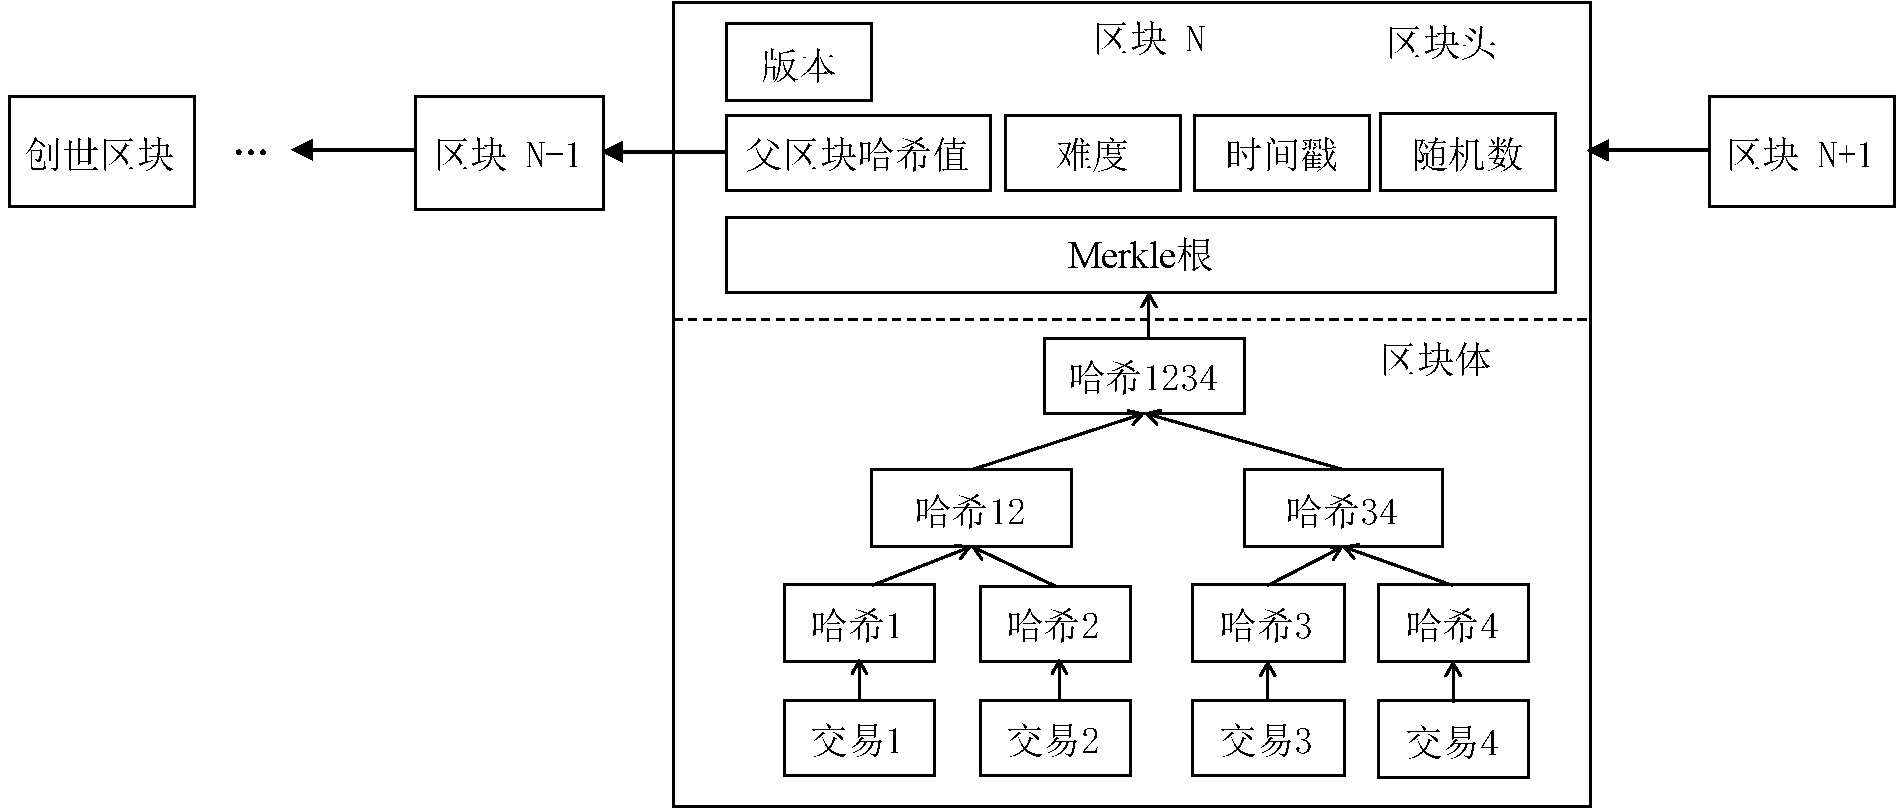
\includegraphics[width=1\textwidth]{FIGs/chapter2/blockchain_example.pdf} %中括号中的参数是设置图片充满文档的大小,你也可以使用小数来缩小图片的尺寸。
    \caption{区块链示例图} %caption是用来给图片加上图题的
    \label{blockchain_example} %这是添加标签,方便在文章中引用图片。
\end{figure}%figure环境

区块链典型示例如图\ref{blockchain_example}所示, 可以看作是一种按照时间顺序将数据区块以顺序相连的方式组合成的一种链式数据结构, 并以密码学方式保证的不可篡改和不可伪造的分布式账本。每个数据区块包含区块头(Block header)和区块体(Block body)两部分, 区块头主要用来存储本区块的一些相关属性, 区块体则用来存储真实的交易数据记录。区块头主要由三组数据组成, 第一组是父区块的哈希值, 用来将该区块与它的前一区块相连接; 第二组数据和矿工竞争挖矿有关, 即难度、时间戳和随机数(Nonce); 第三组是由区块体中计算出来的根哈希值, 即默克尔(Merkle)根。
区块体包括当前区块经过验证的、区块创建过程中生成的所有交易记录。这些记录通过默克尔树的哈希过程生成唯一的默克尔根并记入区块头。整个区块链的第一个区块称为创世区块(Genesis block)。
如果网络中大多数节点通过共识机制就新区块中交易的有效性和区块本身的有效性达成共识, 则可以将新区块添加到链中。

{\footnotesize
\begin{longtable}[h]{m{70pt} m{70pt} m{70pt} m{70pt}}
    \caption[区块链类型]{区块链类型} \label{blockchain_type} \\
        \toprule   
        &\textbf{公有区块链}&\textbf{私有区块链}&\textbf{联盟区块链}\\
        \hline
        准入限制&无&有&有\\
        
        读取者&任何人&仅限受邀用户&相关联用户\\
        
        写入者&任何人&获批参与者&获批参与者\\
        
        所属者&无&单一实体&多方实体\\
        
        交易速度&慢&快&快\\
        \bottomrule
    \end{longtable}
}

当前, 区块链分为公有区块链、联盟区块链和私有区块链。如表\ref{blockchain_type}所示, 公有链没有准入限制, 没有监管方可以组织参与, 任何人都可以参与共识, 常见的两种共识协议为工作量证明机制(Proof of work, 简称PoW)和权益证明机制(Proof of stake, 简称PoS)。由于任何人都可以自由加入, 因此公有链网络具有高度分布式的拓扑结构。但是, 公有链在安全性和性能方面也进行了权衡。公有链上的许多服务器遇到了扩展瓶颈, 吞吐量相对较弱; 与公有区块链的无准入限制形成鲜明对比的是, 私有区块链建立了准入规则, 规定谁可以查看和写入区块链。因为在控制方面有明确的层次结构, 私有链也不是去中心化系统。在某些私有链中, 具备安全模型的背景下,共识协议是多余的。因此在私有区块链中,不使用PoW并不会造成很严重的威胁, 因为每个参与者的身份都是已知的, 是手动进行管理的; 联盟区块链是介于公有链和私有链之间的,结合了两者的特征要素。在共识方面, 联盟链将少数同等权力的参与方视为验证者,而不是像公有链那样开放的系统, 让任何人都可以验证区块, 也不是像私有链那样, 通过一个封闭的系统, 只允许某一个实体来任命区块的生产者。对于从事各类活动的个人和企业来说,存在大量的区块链选择。即使在公有链、私有链和联盟链中,根据复杂性的不同,也会出现许多不同的用户体验。根据实际使用情况,企业可以选择最适合的链实现目标的产品。供应链、电商、医疗等需要彼此之间需要相互沟通的场景下, 联盟链可减轻私有链中交易对手的风险, 并且较少的节点数通常可使它们能够比公共链更有效率的运行, 因此通常选择联盟链。

\subsection{Hyperledger Fabric}
Hyperledger Fabric\footnotemark[1]\footnotetext[1]{\href{https://github.com/hyperledger/fabric}{Hyperledger Fabric}}是一种企业级联盟链解决方案, 因其可插拔模块化、可伸缩、可扩展的架构、多编程语言的智能合约受到业界广泛追捧。

\begin{figure}[h] %figure环境,h默认参数是可以浮动,不是固定在当前位置。如果要不浮动,你就可以使用大写float宏包的H参数,固定图片在当前位置,禁止浮动。
    \centering %使图片居中显示
    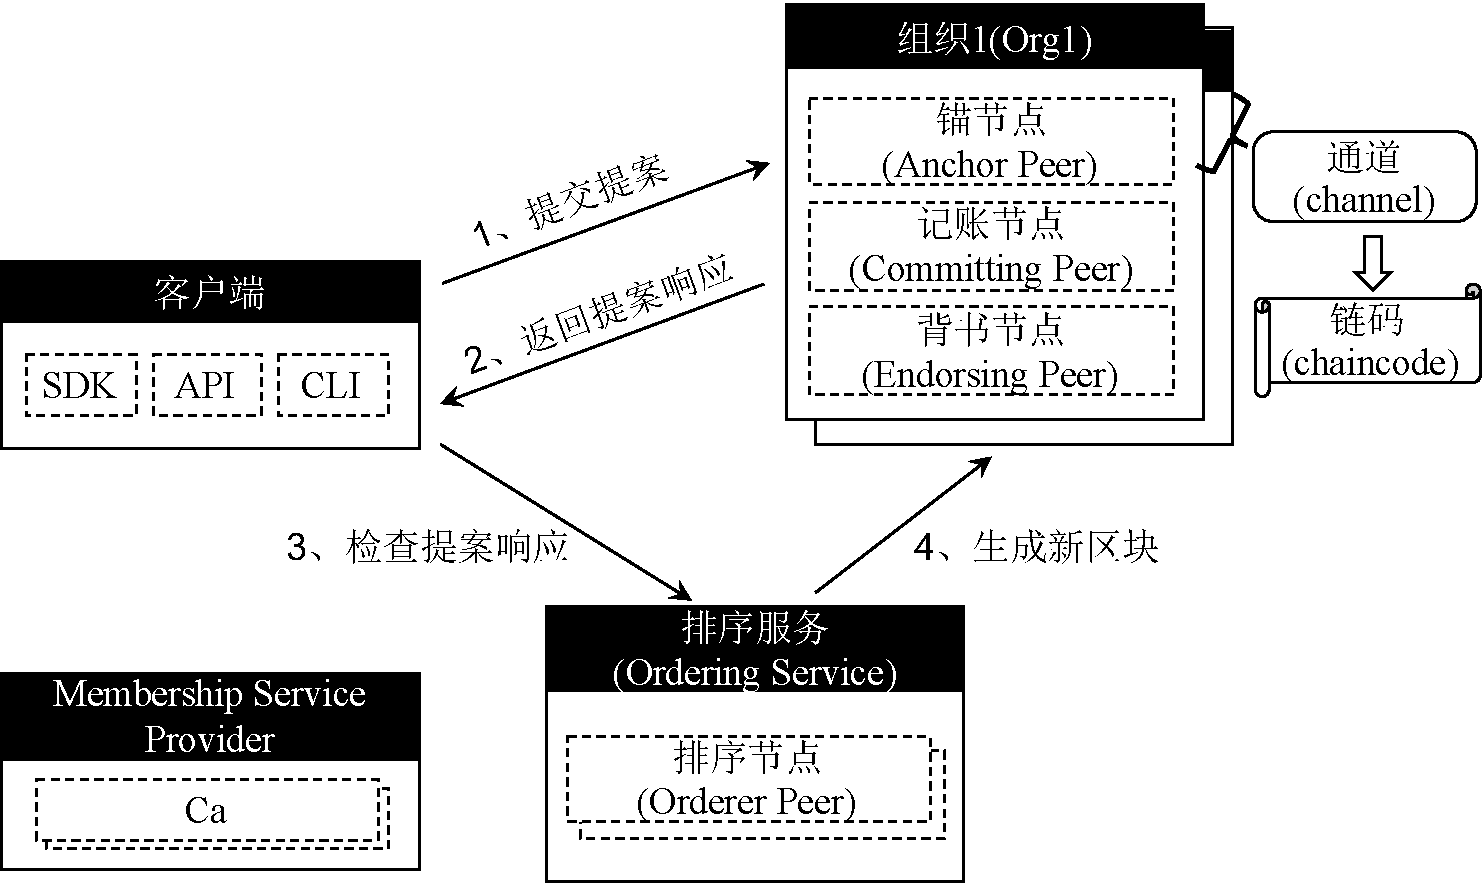
\includegraphics[width=1\textwidth]{FIGs/chapter2/hyperledger_fabric.pdf} %中括号中的参数是设置图片充满文档的大小,你也可以使用小数来缩小图片的尺寸。
    \caption{Hyperledger Fabric网络架构} %caption是用来给图片加上图题的
    \label{hyperledger_fabric} %这是添加标签,方便在文章中引用图片。
\end{figure}%figure环境 

如图\ref{hyperledger_fabric}所示, HF网络通过组织划分, 每个组织内包含多种不同角色的Peer节点, 每个Peer节点又可以担任多种角色, 所有的组织共用排序服务。HF多种节点通过网络相互链接组成联盟链网络完成链上交易。

\textbf{网络节点}
\begin{enumerate}[fullwidth,itemindent=2em,label=(\arabic*)]
    \item 客户端节点: 在HF网络外部用于主动与区块链交互、实现区块链操作的组件。常见的包含软件开发工具包(Software Development Kit, 简称SDK)\footnotemark[2]\footnotetext[2]{\href{https://github.com/hyperledger/fabric-sdk-go}{Hyperledger Fabric Go版本的SDK}}、Fabric-CLI\footnotemark[3]\footnotetext[3]{\href{https://github.com/hyperledger/fabric-cli}{fabric cli}}、REST API\footnotemark[4]\footnotetext[4]{\href{https://github.com/hyperledger/fabric/blob/v0.6/docs/source/API/CoreAPI.rst}{fabric api}};

    \item Ca节点: Fabric-Ca\footnotemark[5]\footnotetext[5]{\href{https://github.com/hyperledger/fabric-ca}{fabric ca}}是一个官方可选的Membership Service Provider组件, 对HF网络中各实体(Identity)的数字身份证书进行管理。完成实体身份注册、数字证书的签发续签或吊销;

    \item Peer节点: HF网络的每个组织都包含一个或多个Peer节点, 每个Peer节点可以通过配置文件担任一种或同时担任多种角色。

    \begin{itemize}[itemindent=2em]
        \item 锚节点(Anchor Peer): 负责与其他组织的锚节点进行通信;

        \item 记账/提交节点(Committing Peer): 负责对区块及区块交易进行验证, 验证通过后将区块写入账本中, 同时提交节点会定期与其他节点通过Gossip协议进行信息交换;

        \item 背书节点(Endorsing Peer): 负责对客户端发送的提案进行签名背书。背书节点与具体的链码(Chaincode)绑定, 其通过调用链码模拟执行交易并向生成提案的客户端返回提案响应。背书节点是动态的, 在客户端发起提案时才会根据背书策略(Endorsement policy)成为背书节点, 其他时候为记账节点。
    \end{itemize}

    \item Orderer节点: 排序服务节点接收经过背书签名的交易并对未打包的交易进行排序生成新区块, 最终通过原子广播到记账节点。排序服务采取支持可插拔设计, 支持Solo、Kafka等分布式共识协议。

\end{enumerate}

HF区块链支持在通信节点之间启用传输层安全性协议(Transport Layer Security, 简称TLS)保证两通信节点的数据保密性和完整性。TLS采用X.509证书进行身份验证并生成会话密钥, 不仅支持客户端节点对服务节点的身份验证, 同时也可以支持服务节点来验证客户端的身份的双向验证。

\textbf{账本结构}

HF中智能合约被称为链码, 通过通道(Channel)允许参与者同时履行不同的链码。HF网络子链通常按照“1个通道+1个账本+N个成员”组成。不同组织及其成员能够在通道中完成特定的交易, 限制信息传播范围。建立一个通道就相当于创建了一条子链, 这条子链上只拥有唯一的一份账本。

\begin{figure}[h] %figure环境,h默认参数是可以浮动,不是固定在当前位置。如果要不浮动,你就可以使用大写float宏包的H参数,固定图片在当前位置,禁止浮动。
    \centering %使图片居中显示
    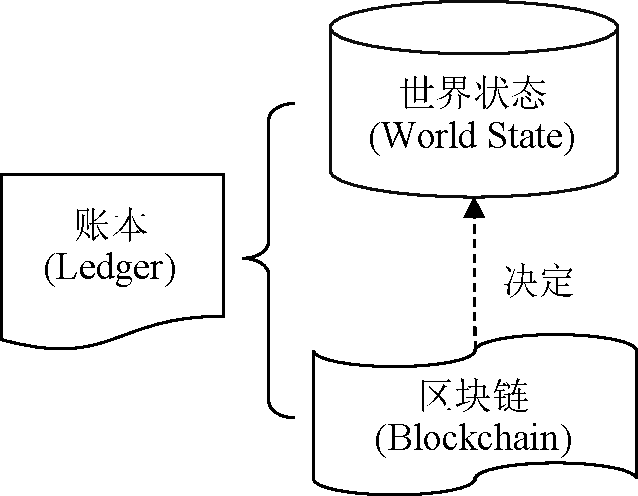
\includegraphics[width=0.45\textwidth]{FIGs/chapter2/ledger.pdf} %中括号中的参数是设置图片充满文档的大小,你也可以使用小数来缩小图片的尺寸。
    \caption{Hyperledger Fabric账本结构} %caption是用来给图片加上图题的
    \label{fabric_ledger} %这是添加标签,方便在文章中引用图片。
\end{figure}%figure环境

如图\ref{fabric_ledger}所示, HF账本由区块链以及世界状态(World State)组成, 其中世界状态由区块链决定。
首先, 世界状态是一个可插拔的键值对(key-value, 简称k-v)数据库, 提供简单、快速、丰富的账本状态检索和存储方式。通过世界状态, 客户端能够直接定位访问账本状态的某个值, 不需要遍历计算整个交易日志。为解决不同类型的问题, HF提供了LevelDB和CouchDB来保障账本状态类型的灵活性。当账本状态是简单的键值对时, 使用LevelDB合适; 当账本状态结构为 JSON时, 使用CouchDB合适。
其次, 这里的区块链指的是交易日志, 是指区块形成的链。区块记录了世界状态改变的历史, 并以文件的方式进行持久化。交易数据一旦写入区块链就无法篡改。

\subsection{Blockchain as a Service}\label{section: BaaS}

\begin{figure}[h] %figure环境,h默认参数是可以浮动,不是固定在当前位置。如果要不浮动,你就可以使用大写float宏包的H参数,固定图片在当前位置,禁止浮动。
    \centering %使图片居中显示
    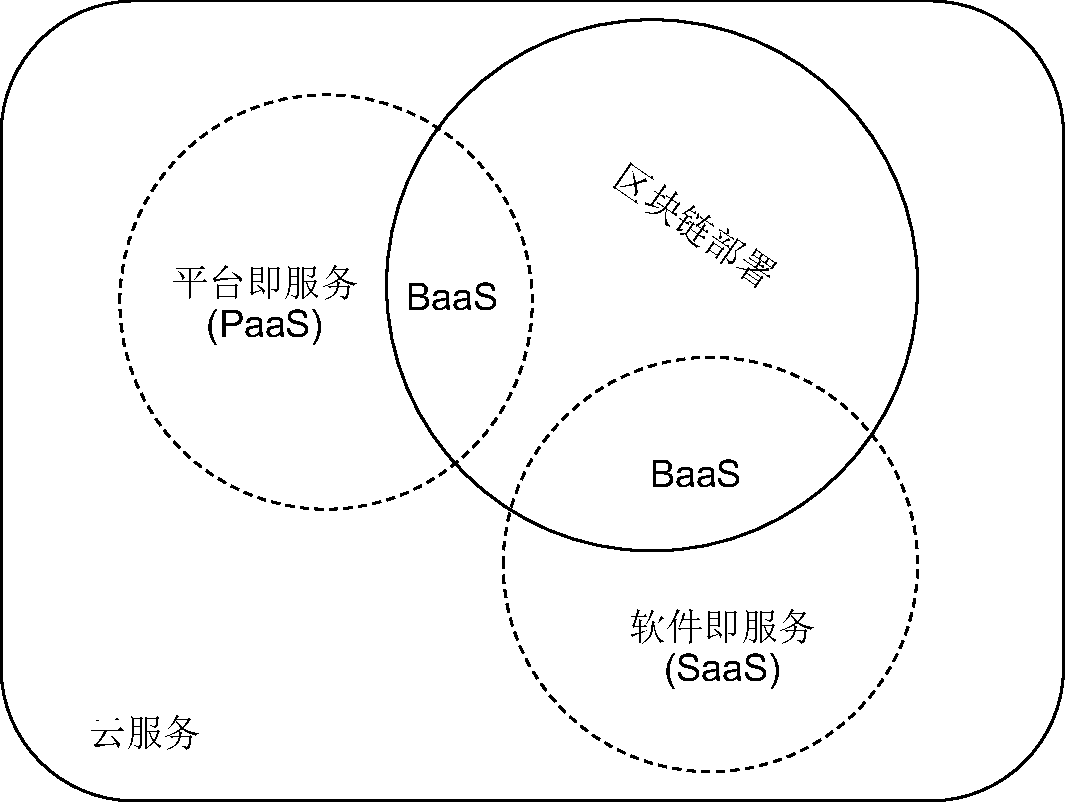
\includegraphics[width=0.55\textwidth]{FIGs/chapter2/BaaS_PaaS_SaaS.pdf} %中括号中的参数是设置图片充满文档的大小,你也可以使用小数来缩小图片的尺寸。
    \caption{BaaS与PaaS以及SaaS的对比} %caption是用来给图片加上图题的
    \label{BaaS_PaaS_SaaS} %这是添加标签,方便在文章中引用图片。
\end{figure}%figure环境

随着区块链以及云原生的发展, BaaS也悄然兴起。云提供了一种抽象、汇集和共享整个网络中的按需的、虚拟的、资源可伸缩的IT环境, BaaS则提供了一种基于云的区块链服务。BaaS能够在云上构建、管理、托管和运维区块链技术, 能够快速部署区块链网络及其开发环境、编写智能合约、构建去中心化应用(即区块链应用, Decentralized application, 简称 Dapp)。基于云基础设施, BaaS屏蔽了底层区块链与云原生的逻辑, 消除了用户构建开发去中心化应用的壁垒, 尤其是部署区块链网络所需的大量硬件和专业知识的前期成本, 为用户提供便捷的、一体化的区块链的能力。如图\ref{BaaS_PaaS_SaaS}所示, 根据BaaS的实施方式, BaaS在云环境中的位置会有所不同\cite{onik2019performance}。BaaS可以从使用平台即服务(Platform as a Service, 简称PaaS)获得基础设施支持的同时也可以通过软件即服务(Software as a Service, SaaS)获得软件服务。

微软推出由Azure云驱动的开放式区块链平台Bletchley, 该项目保证服务对于所有平台、合作者和客户来讲都是开放的、灵活的\cite{BlockchainasaServiceNextGenerationofCloudServices}。IBM推出了名为Bluemix的云计算平台, 依托于PaaS云帮助开发者更快的进行应用开发和部署。随后AWS、Google、阿里云等也相继推出自家的区块链即服务平台。以HF为例, BaaS平台通用的架构如\ref{BaaS_Architecture}所示, 本质上BaaS以计算、存储等资源为基础, 联合上层的区块链基础设施的相关能力, 如共识能力、记账能力、智能合约等转化为可编程接口, 使得区块链网络的部署以及去中心化应用开发过程简单而高效。同时, BaaS通过底层标准化的云基础设施能力为上层的区块链及其去中心化应用提供安全可靠的支撑, 解决弹性、网络、安全性、性能等难题。本文重点关注于基础设施层中Kubernetes上的区块链云化框架的研究。

\begin{figure}[h] %figure环境,h默认参数是可以浮动,不是固定在当前位置。如果要不浮动,你就可以使用大写float宏包的H参数,固定图片在当前位置,禁止浮动。
    \centering %使图片居中显示
    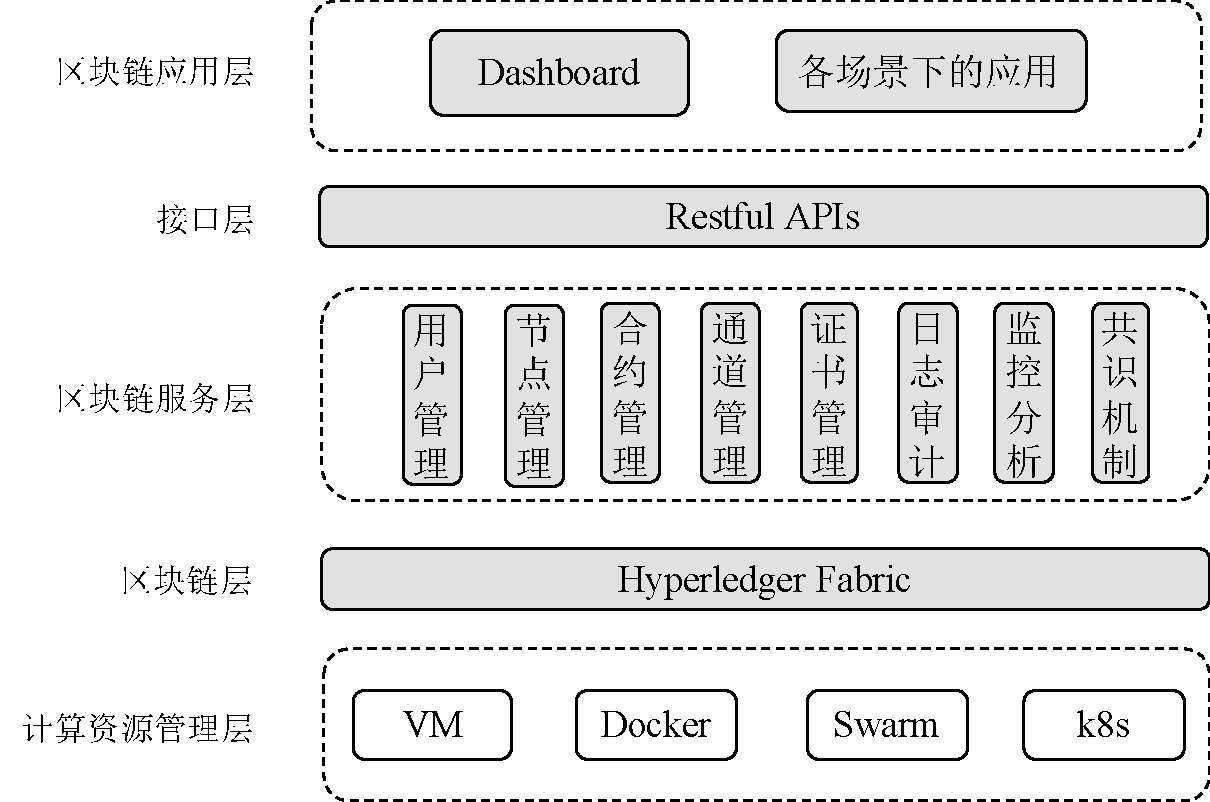
\includegraphics[width=0.85\textwidth]{FIGs/chapter2/BaaS_Architecture.pdf} %中括号中的参数是设置图片充满文档的大小,你也可以使用小数来缩小图片的尺寸。
    \caption{BaaS通用架构} %caption是用来给图片加上图题的
    \label{BaaS_Architecture} %这是添加标签,方便在文章中引用图片。
\end{figure}%figure环境

\section{云原生}\label{section: cloud_native}

\subsection{云原生基本概念}

云原生, 即云原生计算。从发展历程来说, 云原生是云计算的升级。云计算最早由Dell公司在1996年提出\cite{ZHANG20121791}, 亚马逊公司在2006年率先推出的弹性计算云(Elastic Compute Cloud, 简称EC2)服务对云计算产生了深刻影响, 越来越多的企业开始逐步接受云计算这一概念, 并将应用逐步迁移到云端, 享受这一新型计算方式带来的技术红利。此后, 软件系统规模、软件开发方式驱动着技术不断升级。在云计算的时代, 云端只是用于计算的场所, 应用无须重新编写, 只需重新部署, 应用的迁移从物理机到虚拟机, 存储选用兼容的块存储或文件存储。但几乎所有分布式场景中都需应用自行解决稳定性、数据同步、容灾等方面的问题。要解决这些问题, 只能从根本上寻求解决方案。即从迁移到云转变为诞生于云。2013年Docker开源, 之后Pivotal公司提出了云原生的概念, 这是对云计算概念的全面升级。Pivotal指出云原生由容器、微服务、DevOps以及持续交付等技术\cite{WhatisCloudNative}组成, 并充分利用云计算优势构建和运行应用。2014年, 容器编排技术Kubernetes发布。容器技术日趋成熟,在业界开始广泛应用。在2015年, 
云原生计算基金会(Cloud Native Computing Foundation, 简称CNCF)成立。而到了2021年, CNCF已经孵化了超过120个项目、740名成员以及142000的贡献者\footnotemark[1]\footnotetext[1]{\href{https://www.cncf.io/wp-content/uploads/2022/01/CNCF_Annual_Report_2021.pdf}{CNCF2021年年度报告}}。除了工业界, 云原生在学术界也引起了关注, 《计算机学报》发起了以“云原生”为主题的专刊征文\footnotemark[2]\footnotetext[2]{\href{http://chinasoft.ccf.org.cn/papers/7.html}{《计算机学报》云原生软件技术与工程实践专刊征文通知-CCF2021中国软件大会}}。

\begin{figure}[h] %figure环境,h默认参数是可以浮动,不是固定在当前位置。如果要不浮动,你就可以使用大写float宏包的H参数,固定图片在当前位置,禁止浮动。
    \centering %使图片居中显示
    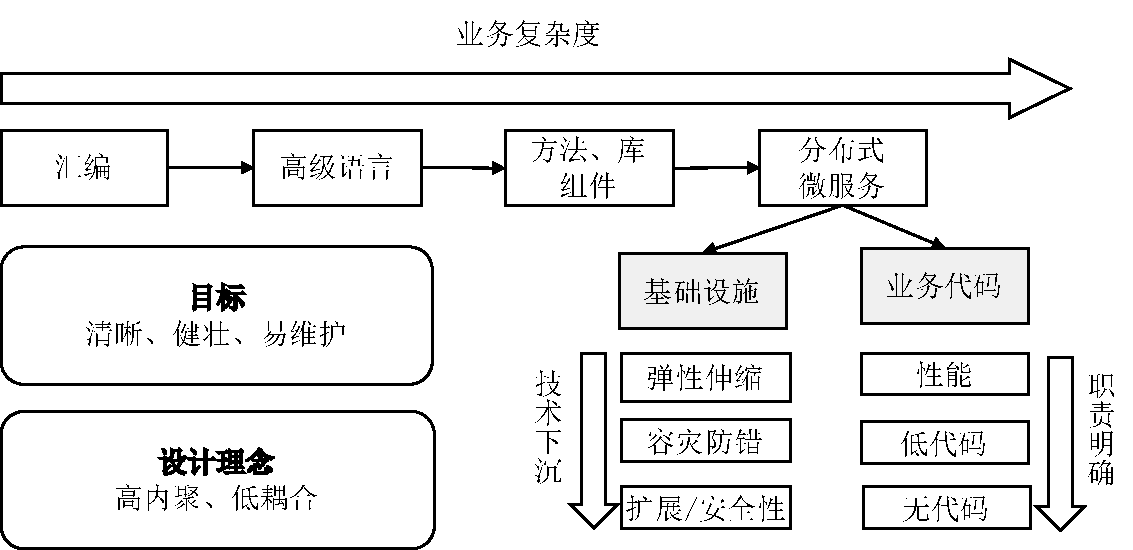
\includegraphics[width=0.9 \textwidth]{FIGs/chapter2/cloud_native_development.pdf} %中括号中的参数是设置图片充满文档的大小,你也可以使用小数来缩小图片的尺寸。
    \caption{云原生技术发展趋势} %caption是用来给图片加上图题的
    \label{cloud_native_development} %这是添加标签,方便在文章中引用图片。
\end{figure}%figure环境

以软件工程的视角来看, 如图\ref{cloud_native_development}所示, 随着软件规模、软件复杂程度在不断增大, 软件上线速度不断加快, 软件稳定性的要求在不断提高。围绕着“高内聚、低耦合”的设计理念, 软件制品进一步深层次抽象, 从单体架构演化为分布式微服务架构, 从可复用的方法、库、组件进一步下沉到底层的基础设施。在这些客观需求的驱动下, 敏捷进一步向运维端延伸, 继瀑布开发、敏捷开发之后, 开发运维一体化(Development and Operations, 简称DevOps)成为又一新兴的软件开发理念和愿景。由于软件体量巨大, 多个不同职责明确的团队负责整体软件项目的运行。DevOps旨在通过一系列文化及技术手段(尤其是自动化IT工具链)打破开发和运维团队之间的壁垒, 改善团队之间的协作关系, 实现更加频繁快速、可靠的软件产品交付\cite{ChinaDevops}。DevOps不仅将敏捷向扩展到运维端, 其更涉及到软件全生命周期中的人、流程与平台。可以说, DevOps是当下软件工程的第一生产力, 其是一种普世的价值观。云原生作为一种基于云基础设施的技术体系涵盖了云应用定义、开发、构建与运行时的所涉及到的各工具或平台。云原生是DevOps生产力下的现阶段生产工具的体现, 是DevOps 的价值具象, “DevOps 时代下的云原生”就如“蒸汽时代的蒸汽机”。

\begin{figure}[h] %figure环境,h默认参数是可以浮动,不是固定在当前位置。如果要不浮动,你就可以使用大写float宏包的H参数,固定图片在当前位置,禁止浮动。
    \centering %使图片居中显示
    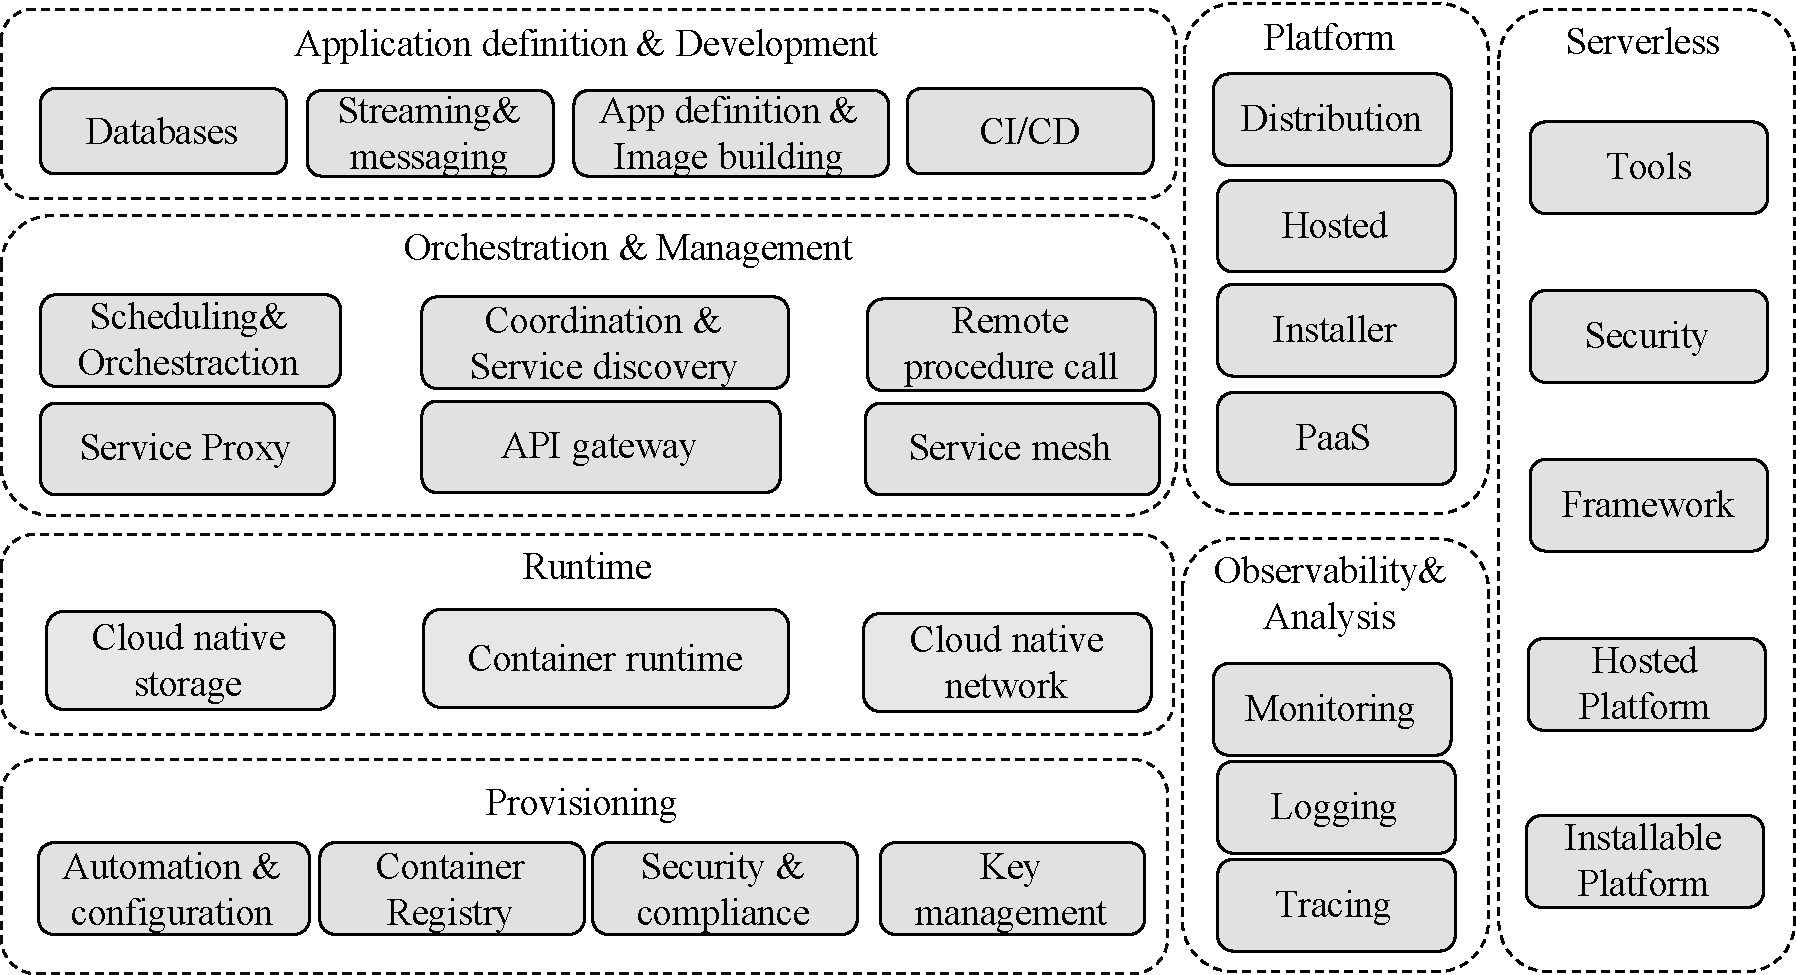
\includegraphics[width=1.0 \textwidth]{FIGs/chapter2/cloud_native_landscape.pdf} %中括号中的参数是设置图片充满文档的大小,你也可以使用小数来缩小图片的尺寸。
    \caption{云原生技术范畴} %caption是用来给图片加上图题的
    \label{cloud_native_landscape} %这是添加标签,方便在文章中引用图片。
\end{figure}%figure环境

云原生技术囊括了DevOps的各环节。如图\ref{cloud_native_landscape}所示, CNCF定义了云原生的技术范畴, 主要包括: 

\begin{itemize}[itemindent=2em]
    \item 供应层(Provisioning): 涉及云原生应用运行环境的自动化基础设施;

    \item 运行时(Runtime): 指保障云原生应用程序正常运行所需的沙盒;

    \item 云应用编排与管理(Orchestration and Management): 为云原生应用提供自动化编排和弹性伸缩能力, 让云原生应用天然地具备可扩展性;

    \item 云应用定义与开发(Application definition and Development): 开发、构建、部署和运行应用程序的工具;

    \item 可观测性与分析(Observability and analysis): 全方位监控和分析云原生应用层的工具;

    \item 平台(Platform): 主要指Kubernetes, 将多类工具有机组合在一起解决庞大的工程问题;

    \item 无服务器(Serverless): 提供函数级别更细粒度部署的一种新的云原生计算模型。
\end{itemize}


随着云架构的不断普及,“未来的软件一定生长于云上”的理念被越来越多的人所接受。云提
供了一种面向企业应用按需进行资源分配的模型, 以一种全新的高效的方式来部署应用。云原生是一系列基于云技术体系和企业管理方法的集合, 既包含了实现应用云原生化的方法论, 也包含了落地实践的关键技术。云原生应用利用容器、服务网格、微服务、不可变基础设施和声明式API等代表性技术, 来构建容错性好、易于管理和便于观察的松耦合系统, 结合可靠的自动化手段可对系统做出频繁、可预测的重大变更, 让应用随时处于待发布状态。Gartner指出, 到2022年全球公共云服务市场预计将增长至约3546亿美元, 60\%的组织将使用外部服务提供商的云管理服务\cite{bhagavan2020achieving}。企业纷纷开始云化转型, 希望将传统应用迁移到云端。

\begin{figure}[h] %figure环境,h默认参数是可以浮动,不是固定在当前位置。如果要不浮动,你就可以使用大写float宏包的H参数,固定图片在当前位置,禁止浮动。
    \centering %使图片居中显示
    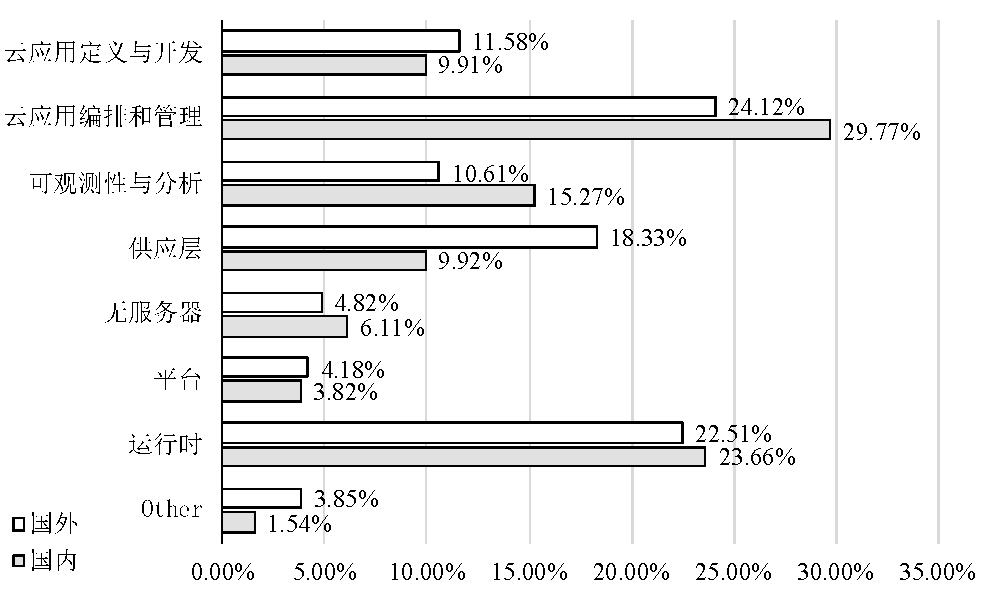
\includegraphics[width=0.9 \textwidth]{FIGs/chapter2/workshop.pdf} %中括号中的参数是设置图片充满文档的大小,你也可以使用小数来缩小图片的尺寸。
    \caption{国内外云原生技术现状} %caption是用来给图片加上图题的
    \label{workshop} %这是添加标签,方便在文章中引用图片。
\end{figure}%figure环境

如图\ref{workshop}所示, 本文根据上述7类云原生技术范畴, 对2020-2021年国内外重点技术会议的共442场分享进行了系统化分析, 其中包括国内云原生社区MeeUp城市站以及Cloud Native+Open Source Virtual Summit China共131场分享, 国际(欧洲、北美)KubeCon+CloudNativeCon Europe以及KubeCon+CloudNativeCon North America 共311篇场分享。从表中可知, 目前国内外研究重点关注于云应用编排以及运行时, 国内对云应用编排与管理的讨论要大于国际并且云应用定义与开发流程、可观测性与分析、平台与无服务器方面国内外相关分享在比例上差距并不是很大, 云原生技术体系已经成为当代软件工程技术发展的主流技术体系。

\subsection{Kubernetes}

Kubernetes(简称k8s)是Google开源的容器集群管理平台。在容器化技术之上, Kubernetes为容器化的云原生应用提供部署运行、资源调度、服务发现、弹性伸缩等一系列基础功能, 提升了大规模容器集群管理的便捷性。自开源来, Kubernetes成为一种全新的基于容器技术的分布式架构解决方案, 在云原生领域具有举足轻重的地位。2019年, 在我国72\%的工程师已经在云原生生产环境中使用大规模使用Kubernetes来进行容器\footnotemark[1]\footnotetext[1]{\href{https://www.cncf.io/blog/2020/10/13/cncf-cloud-native-survey-china-2019/}{CNCF Cloud Native Survey China 2019}}。

\begin{figure}[h] %figure环境,h默认参数是可以浮动,不是固定在当前位置。如果要不浮动,你就可以使用大写float宏包的H参数,固定图片在当前位置,禁止浮动。
    \centering %使图片居中显示
    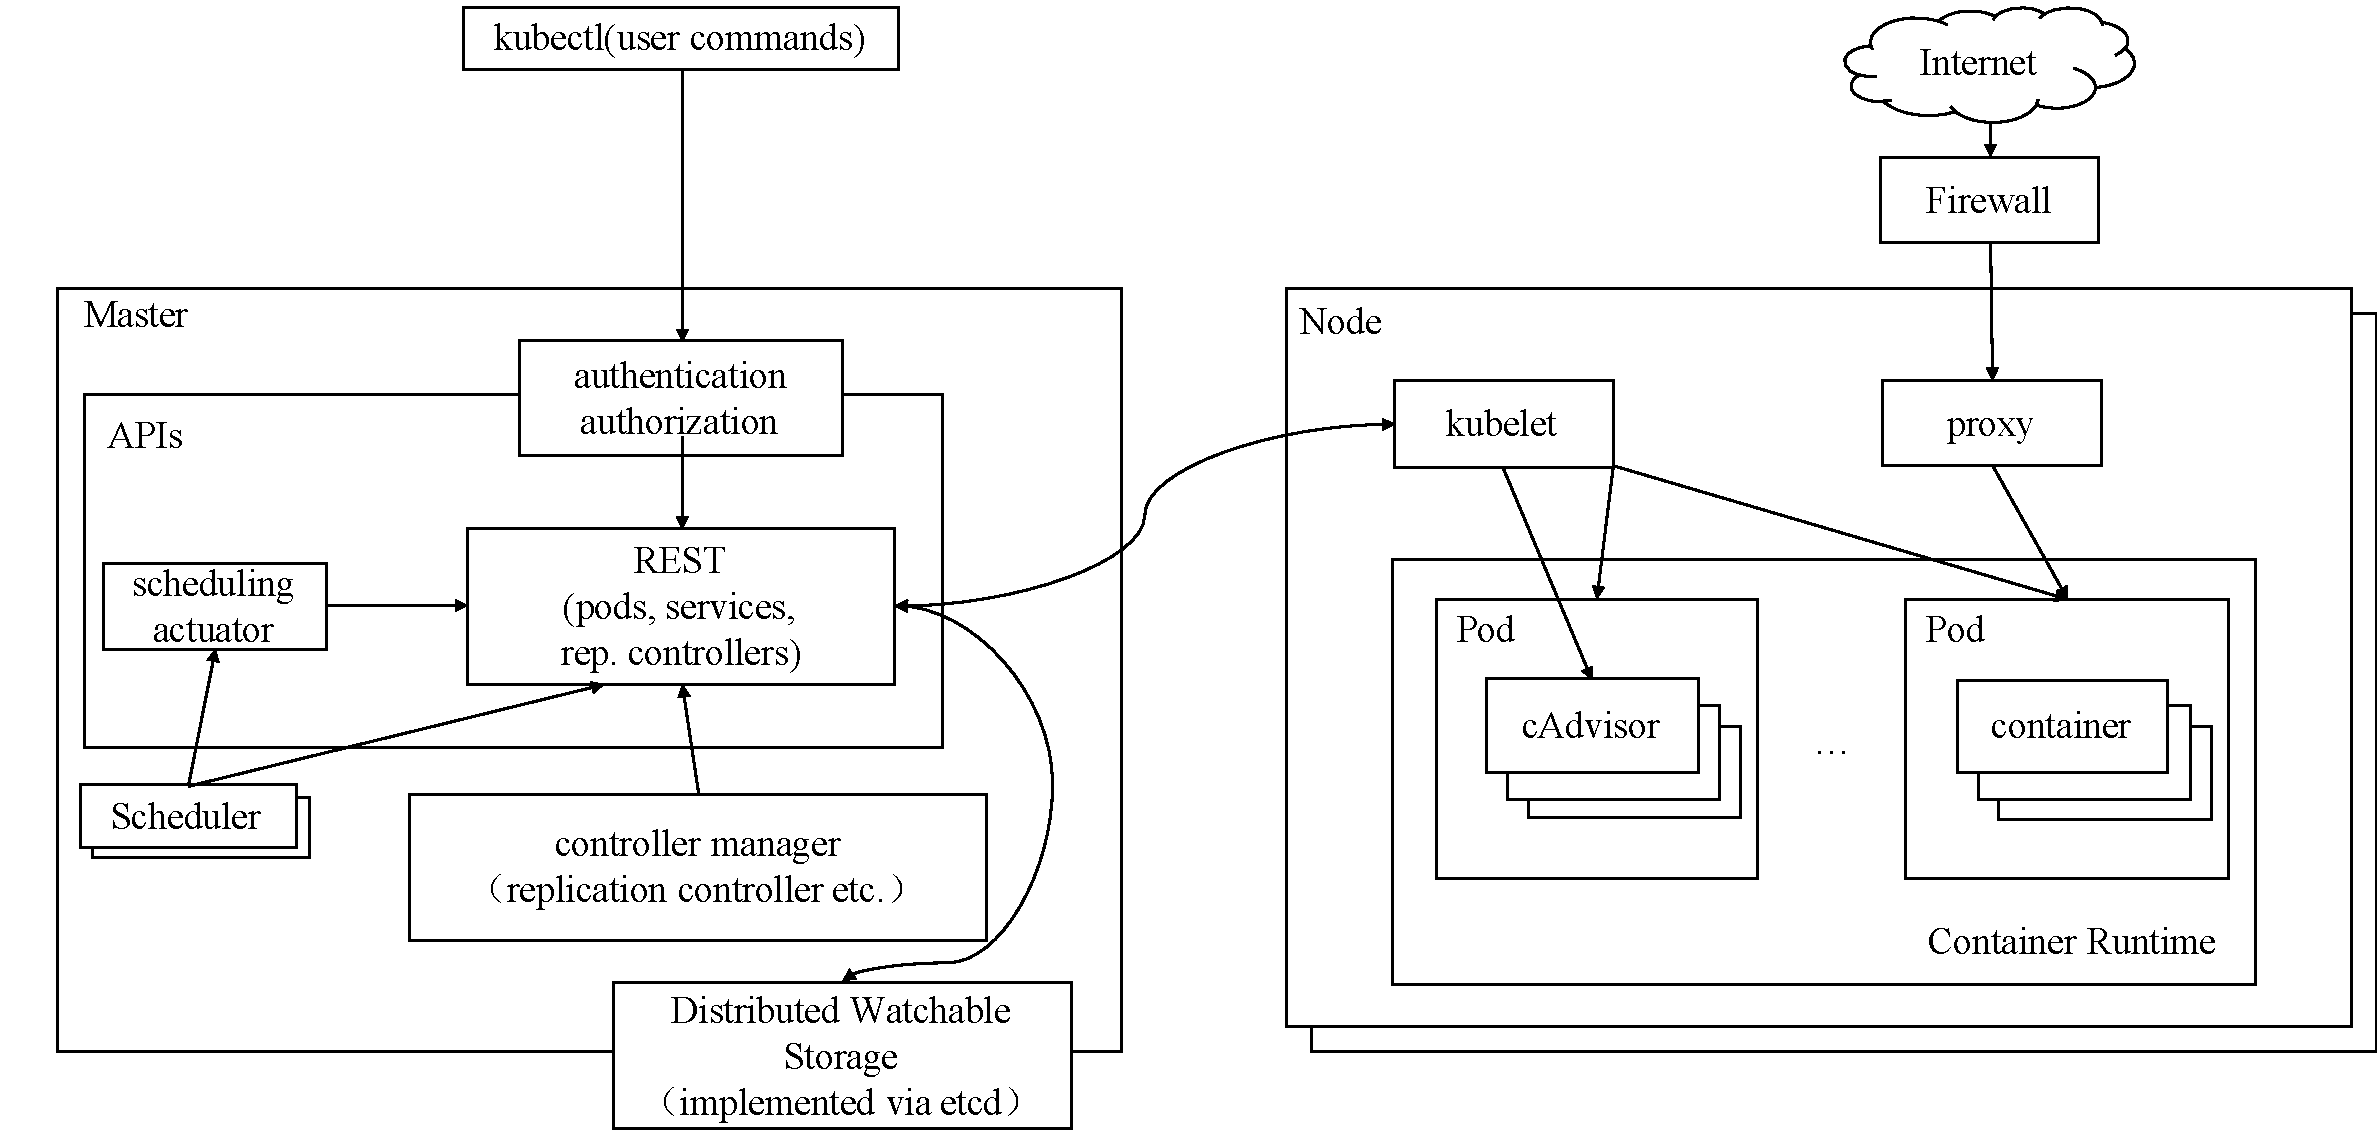
\includegraphics[width=1.0\textwidth]{FIGs/chapter2/k8s.pdf} %中括号中的参数是设置图片充满文档的大小,你也可以使用小数来缩小图片的尺寸。
    \caption{Kubernetes架构图} %caption是用来给图片加上图题的
    \label{k8s} %这是添加标签,方便在文章中引用图片。
\end{figure}%figure环境

Kubernetes由节点代理(kubelet)和Master节点组成。如图\ref{k8s}所示, Kubernetes节点主要由以下核心组件构成:

\begin{itemize}[itemindent=2em]
    \item Etcd: 用于保存集群中一切网络配置和状态信息;

    \item APIServer: 是资源配额控制的入口, 具备完备的集群安全机制并且提供用于集群管理的REST API接口;

    \item Controller Manager: 集群内部的所有资源的管理控制中心, 负责集群内的Node、Pod副本、Endpoint、Namespace、ServiceAccount、ResourceQuota的管理, 实现自动扩展、自动滚动更新、故障检测等功能;

    \item Sheduler: 根据特定的调度算法将Pod调度到指定的工作节点;

    \item kubelet: 定时检查获取节点上Pod、容器的期望状态, 并调用对应的容器平台接口达到这个状态;

    \item Container Runtime: 负责镜像管理以及Pod和容器的真正运作\cite{wangjunxiang2018};

    \item kube-proxy: 为Service提供集群内部的负载均衡和服务发现。
\end{itemize}

Kubernetes拥有独特的声明式API设计, 即声明式地告诉Kubernetes所需资源的状态, 而不是告诉它如何做。在Kubernetes中对象(Object)是持久化的实体, Kubernetes使用这些实体去表示整个集群的状态, 同时这些对象可以在Yaml\cite{ben2009yaml}文件中作为一种声明式API类型来灵活的创建并配置。典型的, Kubernetes的对象主要有以下几种: 

\begin{itemize}[itemindent=2em]
    \item Namespace: 能够隔离资源。Kubernetes集群可以拥有多个命名空间, 这些命名空间在逻辑上彼此隔离, 实现了对多用户的资源隔离;

    \item Pod: Kubernetes中最基本的操作单元, 包含一个或多个容器。Kubernetes为每个Pod分配一个唯一的IP地址, Pod内部的多个容器共享该IP地址。并且每个Pod都能设定自己的计算资源, 即CPU和Memory;

    \item Replication Controller(简称RC): 确保任意时间Kubernetes集群中运行指定数量的Pod副本;

    \item Deployment: 保证Pod的数量和健康, 绝大多数的功能与RC完全一样, 能够被当作全新一代的RC;

    \item Service: 定义了一个Pod逻辑集合以及访问Pod的策略, 它提供一种桥梁会为访问者提供一个固定的Pod访问地址用于在访问时重定向到相应的后端;

    \item Label: 通过键值对的方式被附加到任何资源对象上, 用于配置资源;

    \item Secret: 不需要将敏感数据外露, 解决密码、token、密钥等敏感数据的配置问题;

    \item Role: 一组权限的集合, 给某个NameSpace中的资源进行鉴权;

    \item ConfigMap: 为了让镜像和配置文件解耦, 应用程序会从配置文件、命令行参数或环境变量中读取配置信息,以便实现镜像的可移植性和可复用性;

    \item Volume: Pod中能够被多个容器访问的持久化共享目录;

    \item Persistent Volume(简称PV): 类似于Volume, Kubernetes提供的存储资源的抽象管理集群存储, 其API内包含存储的细节实现;

    \item Persistent Volume Claim(简称PVC): 对存储资源的请求声明, PVC不关心底层存储实现的细节, 只消耗PV资源。

\end{itemize}

随着Kubernetes生态的持续发展, 上述常规的资源类型仅代表通用的对象, 并不能适应多变的业务需求。为提升自身的扩展能力, Kubernetes提供用户自定义CRD向Kubernetes API中增加定制化的资源类型。用户的自定义资源(Custom Resource, 简称CR)创建并注册到Kubernetes API后, 其与常规通用资源对象都是原生的、存在于etcd中的同等资源, 可以采用Kubernetes原生方式进行创建、查看。CRD本质上用于声明用户自定义资源对象, 开发人员还需要针对CRD提供关联的Operator对CR进行完整生命周期管控。

Operator主要负责有状态应用(即CR)及其组件的部署、更新、自动扩展、维护、数据备份等, 保证其可用性。其作为Kubernetes的一种扩展形式, 基于Kubernetes的资源和控制器(Controller)概念构建, 遵循Kubernetes原则, 功能类似于Controller Manager, 但同时又注入了特定领域知识。

\section{其他相关技术}\label{section: other_technologies}

\subsection{Helm}

Helm是一种基于Kubernetes云计算平台的打包和部署复杂软件应用程序的技术\cite{spillner2019quality}。随着云原生及微服务架构的发展, 开发人员倾向于将大的单体应用分解成多个可以独立开发、部署、运维的微服务部署于Kubernetes之上。服务数量的增加为Kubernetes编排带来了复杂性, Helm则通过软件打包的方式极大的简化了Kubernetes应用部署和管理的复杂性。

Helm存在三个核心概念:

\begin{itemize}[itemindent=2em]
    \item chart: 即一系列包含创建Kubernetes应用实例必要信息的文件;

    \item config: 包含应用发布的相关配置信息;

    \item release: chart及其配置的运行实例。
\end{itemize}

如图\ref{helm}所示, Helm将Kubernetes资源(如Deployment、Service)打包到chart中, chart将会被保存到仓库中。Tiller是部署于Kubernetes中的Helm的服务端, 负责接受Helm请求并于APIServer进行交互, 根据chart生成并管理release。开发者使用Helm可以简化应用配置及版本管理, 使得在Kubernetes上部署、升级、回滚、卸载应用程序更加方便。

\begin{figure}[h] %figure环境,h默认参数是可以浮动,不是固定在当前位置。如果要不浮动,你就可以使用大写float宏包的H参数,固定图片在当前位置,禁止浮动。
    \centering %使图片居中显示
    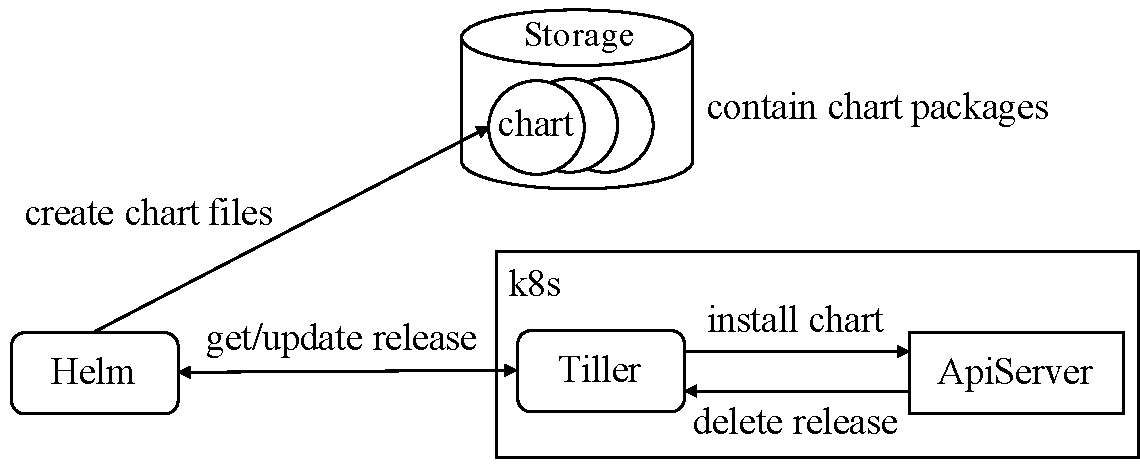
\includegraphics[width=0.8\textwidth]{FIGs/chapter2/helm.pdf} %中括号中的参数是设置图片充满文档的大小,你也可以使用小数来缩小图片的尺寸。
    \caption{Helm架构图} %caption是用来给图片加上图题的
    \label{helm} %这是添加标签,方便在文章中引用图片。
\end{figure}%figure环境

% \subsection{Istio}

% 随着技术下沉, 传统由软件本身负责的负载均衡、路由等功能下沉到云原生基础设施。服务网格(Service Mesh)通过在不断变化的条件和拓扑结构面前强制执行所需的网络行为, 为网络连接的工作负载提供基于策略的网络服务\cite{calcote2019istio}。Istio\footnotemark[1]\footnotetext[1]{\href{https://github.com/istio/istio}{istio}}是Service Mesh架构的一种实现方式, 其是一个用于保证容器服务间连接、安全、控制和观测的网络代理组件, 具有负载均衡、服务间认证、监控等功能。

% Istio分为两个逻辑部分\cite{larsson2020impact}: 数据平面(Data Plane)与控制平面(Control Plane)。数据平面由代理程序Envoy(通常被称为Sidercar)组成, 其受控制平面组件控制, 通常与业务容器捆绑, 来劫持业务应用容器的流量完成针对特性应用程序的控制与治理; 控制平面提供服务发现、配置和证书管理等功能, Istio对其进行了进一步细分:

% \begin{itemize}[itemindent=2em]
%     \item Mixer: 负责策略、访问控制和请求追踪;

%     \item Pilot: 提供服务发现的功能;

%     \item Citadel: 负责证书颁发;
% \end{itemize}

\section{本章小结}

本章\ref{section: blockchain}节首先介绍了区块链基本概念、架构、分类, 其次重点介绍联盟链解决方案HF的网络节点、账本结构, 最后介绍区块链即服务的诞生和通用架构; \ref{section: cloud_native}节介绍云原生的发展历程、技术范畴以及Kubernetes; \ref{section: other_technologies}节介绍本文区块链云化架构涉及到的其他相关技术。

% \begin{figure}[!htbp] %figure环境,h默认参数是可以浮动,不是固定在当前位置。如果要不浮动,你就可以使用大写float宏包的H参数,固定图片在当前位置,禁止浮动。
%     \centering %使图片居中显示
%     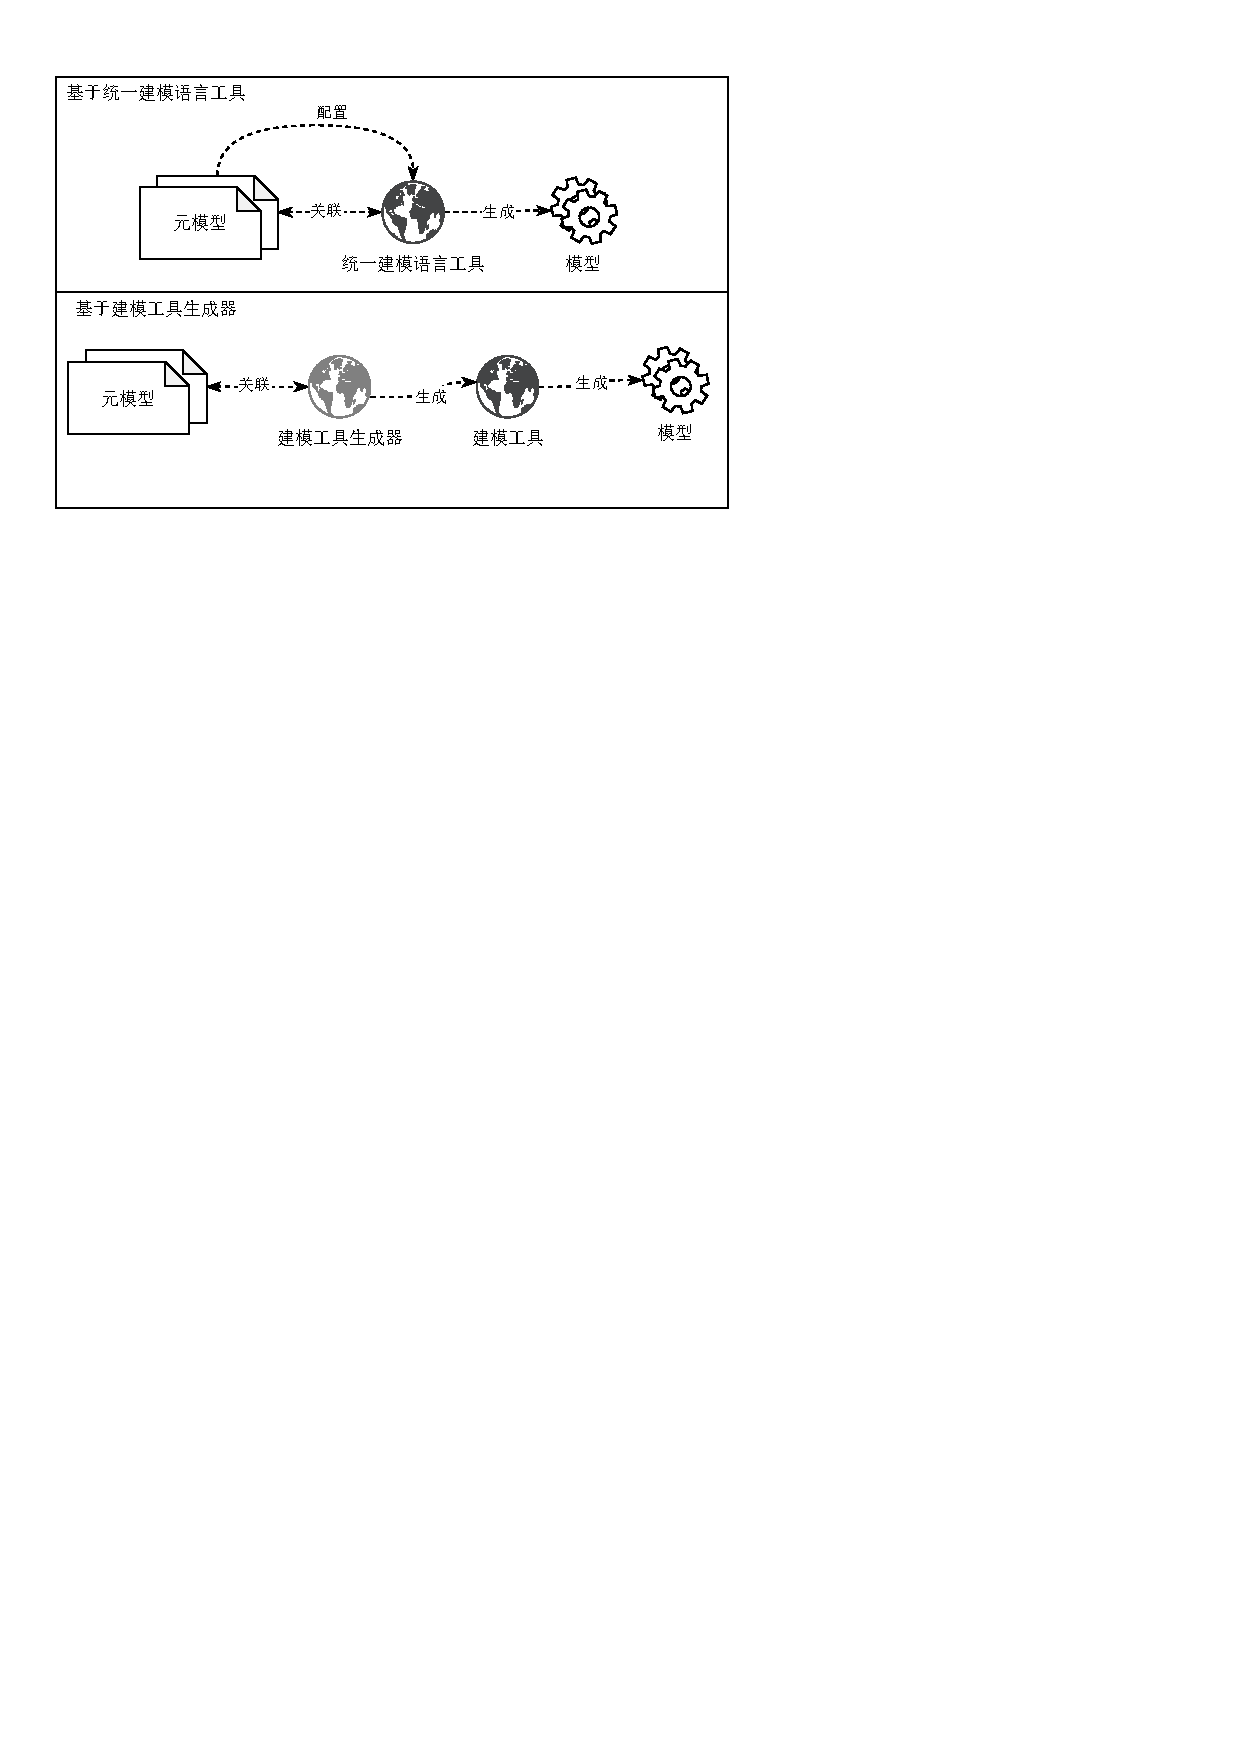
\includegraphics[width=0.8\textwidth]{FIGs/chapter3/2kindsmodeling.pdf} %中括号中的参数是设置图片充满文档的大小,你也可以使用小数来缩小图片的尺寸。
%     \caption{两种建模工具实施方式} %caption是用来给图片加上图题的
%     \label{2kindsmodeling} %这是添加标签,方便在文章中引用图片。
% \end{figure}%figure环境







\chapter{区块链云化框架调研分析}

本章首先通过快速评审获得Kubernetes operator赋能质量属性的策略集,  随后阐述区块链云化框架的设计原则, 最后结合区块链去中心化等特性以及设计原则分析筛选策略集形成基于Hyperledger Fabric的区块链云化框架的核心具体实施方案。

\section{快速评审}\label{section: rapid_reviews}

软件工程中, 快速评审(Rapid reviews)是一种轻量级的二级研究, 以实践为导向专注于及时的向研究人员提供证据\cite{cartaxo2020rapid}。本文对已发表的学术文章进行快速评审, 快速评审的目的是为了在较短时间内了解目前学术界使用Kubernetes operator进行云化的现状, 以及如何使用Kubernetes对现有系统进行赋能。随后, 对应文献对快速评审所得到的结果进行整理归纳得到Kubernetes operator如何为质量属性赋能的策略集。

本文的快速评审过程分为以下步骤: 首先进行自动化的全文数据库检索, 再筛选出与Kubernetes operator及架构改造强相关的文献, 接下来提取出本文所关注的质量属性及相关策略, 最后归纳整理出策略集。

{\footnotesize
\begin{longtable}[h]{m{60pt} m{210pt} m{40pt}<{\centering}}
    \caption[每个全文数据库的搜索字符串]{每个全文数据库的搜索字符串} \label{search_string} \\
        \toprule  
        \textbf{全文数据库}&\textbf{搜索字符串}&\textbf{文献数}\\
        \hline
        IEEE Xplore &(“kubernetes AND operator”) OR (“k8s AND operator”) OR (“custom resource defination”) & 23 \\

        ACM & “kubernetes operator” OR “k8s operator” & 7 \\

        Springer &((“kubernetes AND operator”) OR (“k8s AND operator”))AND ((“custom resource defination”) OR "CRD") & 0 \\

        ScienceDirect &(“kubernetes AND operator”) OR (“k8s AND operator”) OR (“custom resource defination”) & 0 \\
        \hline
        Scoups\&Google &“kubernetes operator”& 21(去重) \\
        \bottomrule
    \end{longtable}
}

如表\ref{search_string}所示, 为全面获取学术届对基于Kubernetes operator云化的策略, 确定了本次检索的全文数据库以及搜索字符串。本次检索主要针对计算机与软件工程领域的全文数据库\cite{lisboa2010systematic}(包含ACM、IEEE Xplore、Springer、ScienceDirect), 同时检索Scoups以及谷歌学术进行补充。最终, 围绕“kubernetes operator”为检索主题得到的共51篇论文。在文献筛选阶段, 本文根据筛选标准筛选出15篇与Kubernetes operator云化强相关的文献, 入选文献如表\ref{rapid_reviews}所示。文献筛选标准主要有:

\begin{itemize}[itemindent=2em]
    \item 论文的主要目的是利用Kubernetes对原有系统进行云化;

    \item 论文针对于Kubernetes operator方法;

    \item 论文介绍了具体的改造策略及相关的质量属性。
\end{itemize}

{\footnotesize
\begin{longtable}[h]{m{40pt} m{280pt} m{40pt}<{\centering}}
    \caption[快速评审入选文献列表]{快速评审入选文献列表} \label{rapid_reviews} \\
        \toprule  
        \textbf{文献编号}&\textbf{文献标题}&\textbf{文献引用}\\
        \hline
        [P1]&Enhancement of observability using Kubernetes operator&\cite{Shenoy2022496}\\
        
        [P2]&Designing a Kubernetes Operator for Machine Learning Applications&\cite{kanso2021designing}\\
        
        [P3]&Container orchestration on HPC systems through Kubernetes&\cite{zhou2021container}\\
        
        [P4]&Validation and Benchmarking of CNFs in OSM for pure Cloud Native applications in 5G and beyond&\cite{pino2021validation}\\
        
        [P5]&On-the-fly fusion of remotely-sensed big data using an elastic computing paradigm with a containerized spark engine on kubernetes&\cite{huang2021fly}\\
        
        [P6]&A Role-Based Orchestration Approach for Cloud Applications&\cite{yue2021role}\\
        
        [P7]&A Design of MANO System for Cloud Native Infrastructure&\cite{lee2021design}\\
        
        [P8]&Dynamic Updates of Virtual PLCs Deployed as Kubernetes Microservices&\cite{koziolek2021dynamic}\\

        [P9]&Suture: Stitching safety onto kubernetes operators&\cite{mahajan2020suture}\\
        
        [P10]&Automation of virtualized 5G infrastructure using mosaic 5G operator over kubernetes supporting network slicing&\cite{wiranata2020automation}\\
        
        [P11]&5G Cloud-Native: Network Management \& Automation&\cite{arouk20205g}\\
        
        [P12]&Proposed model for distributed storage automation system using kubernetes operators&\cite{sharma2020proposed}\\
      
        [P13]&Monitoring Resilience in a Rook-managed Containerized Cloud Storage System&\cite{baumann2019monitoring}\\
        
        [P14]&Reproducible Benchmarking of Cloud-Native Applications With the Kubernetes Operator Pattern&\cite{henning2021reproducible}\\
        
        [P15]&Pivotal Greenplum©for Kubernetes: Demonstration of Managing Greenplum Database on Kubernetes&\cite{patel2019pivotal}\\
        \bottomrule
    \end{longtable}
}

在数据提取阶段, 本文对5个提取项(文献标题、文献发表年份、质量属性、策略、所属领域)进行抽取, 共得到44条针对不同质量属性的相关策略。在数据归纳阶段, 由于不同的文献中对语义相同的质量属性用词存在明显差异, 本文根据国际软件质量评价标准ISO/IEC 25010:2011\footnotemark[1]\footnotetext[1]{\href{https://www.iso.org/standard/35733.html}{ISO/IEC 25010:2011 System and software quality models}}所定义的质量模型对收集到的文献中表述的质量属性进行映射, 同时对相同或相似的策略进行整理合并, 得到策略集如表所示。

{\footnotesize
\begin{longtable}[h]{m{40pt}|m{40pt}|m{20pt}|m{150pt}|m{80pt}}
    \caption[基于Kubernetes operator云化策略集]{基于Kubernetes operator云化策略集} \label{policy_set} \\  
        \hline
        \textbf{文献中质量属性}&\textbf{ISO质量属性}&\textbf{编号}&\textbf{策略}&\textbf{参考文献}\\
        \hline
        \multirow{4}*{\parbox[c]{40pt}{生产效率 \\ 效率}} & \multirow{4}*{易用性}
        &S1&容器化及Kubernetes能力 & [P3] \\\cline{3-5}
        & &S2&自动化配置复杂领域知识 & [P1, P2, P12-15] \\\cline{3-5}
        & &S3&自动化构建、部署应用程序 & [P6, P10, P11] \\\cline{3-5}
        & &S4&operator与helm结合 & [P1, P4, P13] \\\cline{3-5}

        \hline
        可迁移性 & 适应性
        &S1&容器化及Kubernetes能力 & [P1-P3, P8, P10-P12] \\\cline{3-5}

        \hline
        \multirow{2}*{可用性} & \multirow{2}*{可靠性}
        &S1&容器化及Kubernetes能力 & [P2, P15] \\\cline{3-5}
        & &S5&主备切换 & [P15] \\\cline{3-5}

        \hline
        \multirow{3}*{\parbox[c]{40pt}{可扩展性 \\ 可伸缩性 \\ 灵活性}} & \multirow{3}*{无}
        &S1&容器化及Kubernetes能力 & [P2, P3, P5, P7, P12, P15] \\\cline{3-5}
        & &S6&基于监控指标并进行伸缩处理 & [P2, P6, P13] \\\cline{3-5}
        & &S7&链外利用存储即服务 & [P15] \\\cline{3-5}

        \hline
        \multirow{4}*{安全性} & \multirow{4}*{安全性}
        &S8&RBAC & [P2] \\\cline{3-5}
        & &S9&自定义访问控制机制 & [P9] \\\cline{3-5}
        & &S10&多用户认证授权机制 & [P3, P13] \\\cline{3-5}
        & &S11&资源隔离 & [P13] \\\cline{3-5}

        \hline
        \multirow{1}*{可监控性} & \multirow{1}*{无}
        &S12&基于Prometheus的监控体系 & [P1, P5, P12, P13] \\\cline{3-5}
        \hline
    \end{longtable} 
}

\section{设计原则}\label{section: framework_characteristics}

区块链云化框架致力于在BaaS一站式构建、管理、托管和运维区块链网络及其应用的基础上更深入云原生底层基础设施Kubernetes的底层, 有效利用云能力对Fabric基础设施赋能, 需要满足以下原则:

\begin{itemize}[itemindent=2em]
    \item 易用性: 在Kubernetes上启动管理Hyperledger Fabric网络并部署链码需要专业的领域知识, Fabric各组件的配置项繁多且与Kubernetes适配极易出错。区块链云化框架需屏蔽底层Fabric配置与Kubernetes逻辑, 帮助用户采用命令行配置的方式提供完整的Fabric各组件的全生命周期管理;

    \item 可迁移性: 区块链云化框架需要具备基础架构的云独立性, 本框架依托Kubernetes, 可以方便的迁移到支持Kubernetes的任何云;

    \item 可视运维: 当前区块链系统缺乏一套涵盖不同层面的标准方法来监控区块链及其智能合约的运行\cite{zhangfuli2021smartcontract}。 区块链云化框架需提供基本运维能力, 有效复用云上监控方案为区块链系统提供7*24小时可视化资源监控能力;

    \item 安全性: 区块链云化框架需要具备有效的认证、鉴权、准入机制来确保区块链系统的安全性; 具备可插拔的共识算法取保区块链的去中心化、可追溯等特点, 支持完善的用户密钥授权、保存、隔离处理以及提供可靠的故障恢复能力;

    \item 可扩展性: 区块链云化框架需按照模块化配置, 将Kubernetes底层的计算资源、存储资源、网络资源等供给Fabric, Fabric的Ca、Peer、Orderer基本组件的证书认证、共识、TLS加密、存储等功能模块作为可配置项进行命令式配置; 该框架能够确保系统核心底层逻辑稳定运行的同时, 对外提供小而精的扩展边界, 实现系统的高内聚与低耦合;

    \item 透明性: 区块链云化框架需保证区块链上所有的交易记录是可追溯的、不可篡改的, 区块链交易过程以及获取交易产生的记录需要专业人员才能获取操作, 非专业人员难以理解, 框架需通过简单透明的方式获取交易记录。
\end{itemize}

\section{策略集应用}\label{section: policy_set_application}

通过快速评审的方式形成的基于Kubernetes operator云化策略集作为可选指导方案, 需要贴合区块链领域自身约束才能有效纳入区块链云化框架中落地。本节将围“所选策略为何能提升质量属性”以及“所选策略是否适用于Fabric”进行阐述。

容器化在云原生应用程序中的拥有更高的部署效率\cite{zhou2021container}、可迁移性。容器化可以使每个软件应用程序在隔离的环境中运行, 其将应用程序及其库、配置文件和其他依赖项封装在一起, 确保了环境兼容性, 从而使用户能够轻松地在不同的环境中移动和部署程序。因此, 容器化使得应用程序具备极强的可迁移性。Docker\footnotemark[1]\footnotetext[1]{\href{https://www.docker.com/}{Docker官网}}是容器化的典型代表, 其可以将运行态的容器打包成镜像(image)并储存在在线存储仓库中。Docker容器不是虚拟机, 这意味着它可以使用宿主机现有的网络接口\cite{shah2019building}。一旦创建了容器, 就可以为容器提供一个专用环回接口, 用于内部通信, 完成部署。

Kubernetes作为容器管理调度平台, 其具备强大的调度、伸缩和自恢复能力。Kubernetes会自动打包应用程序, 并根据预设需求运行Pod并管理容器。利用自身机制, Kubernetes可以轻松的将Pod进行横向扩容(Horizontal Pod Autoscaler, 简称HPA)或纵向扩容(Vertical Pod Autoscaler, 简称VPA)。Kubernetes提供了强大的容器自恢复能力, 可以自动重启在执行过程中失败的容器, 并杀死那些没有响应用户定义的健康检查的容器。但如果节点本身死亡, 那么它会替换并重新安排发生故障的容器到其他可用节点上。

Hyperledger Fabric官方提供了Binaries和Docker镜像两种安装方式\footnotemark[1]\footnotetext[1]{\href{https://github.com/hyperledger/fabric/blob/main/scripts/bootstrap.sh}{fabric\_bootstrap.sh}}, 其天然的满足容器化构建。一旦Fabric以镜像的方式托管于Kubernetes, 即可原生的利用Kubernetes进行高可用的管理。

值得注意的是, 区块链网络是去中心化的网络, 所有的节点共同参与记账, 只需要网络中的大多数(超过51\%)节点的账本状态一致即可, 并不需要所有网络中的所有的节点时刻保持高可用状态。同时, 无论是基于Kubernetes的多副本伸缩还是基于监控指标进行伸缩仅保证的是无状态应用的高可用性, 并不解决数据一致性问题, 所以为某个Fabric节点增加多副本进行可伸缩意义不大, 利用Kubernetes的自恢复能力保证单Fabric节点可用即可。

Blockchain Automation Framework采用脚本方式将Fabric部署于Kubernetes, 仅仅成了一次性自动化构建、部署Fabric的任务。这虽然能在一定程度上提升Fabric网络的部署效率, 但这不仅无法将Fabric复杂的领域知识以插拔化的方式配置进入云基础设施内部而且与helm的弊端一样, 不能对已经部署完成的Fabric网络各节点进行完整软件生命周期管理。Kubernetes operator提供的CRD方式可以插拔式地领域知识注入进云基础设施内部, 降低了Kubernetes运维人员对Fabric网络的二次学习成本。通过operator与Fabric helm的结合不仅能够提升Fabric网络的部署效率, 也可以时刻监听helm状态实现对整个网络进行完整生命周期管理。

虽然针对Peer节点的可伸缩性意义不大, 但从海量数据存储的角度来看, 使用云存储是加强区块链网络存储一种替代方法, 它减少了因区块存储空间有限而造成的限制\cite{gai2020blockchain}。云可以为区块链网络提供提供存储即服务(Storage as a Service, 简称SaaS)作为一种可扩展的链外解决方案。Kubernetes的SaaS通过服务的形式精细化使用存储资源, 实现了对存储定义(PVC)和存储申请(StorageClass)的灵活分离。Fabric网络的世界状态是一种脱链的链外附加缓存机制, 其最终被保存在链外的LevelDB或CouchDB中。同时, 世界状态的丢失并不会对区块链中的数据产生影响。这种链外存储机制可以使得Fabric网络能够通过Kubernetes的SaaS机制挂载外部存储单元不必关心存储资源的实际物理位置, 能够做到存储资源的即插即用。 

安全性方面, 区块链领域频繁的出现安全问题可能会动摇人们对去中心化应用的信任, 访问控制是提供云数据安全和隐私的一种基本方法, 可以防止未经授权的用户侵入云数据。不可靠的访问控制方法也会影响其他功能, 如身份验证、授权和数据审核。除自定义访问控制机制外, 云中的传统访问控制方法主要基于成熟的访问控制策略, 现有的传统访问控制策略分为四种: 自主访问控制(Discretionary Access Control, 简称DAC)、强制访问控制(Mandatory Access Control, 简称MAC)、基于角色的访问控制(Role-Based Access Control, 简称RBAC)和基于属性的访问控制(Attribute-Based Access Control, 简称ABAC), 其对比如表\ref{access_control}所示。

{\footnotesize
\begin{longtable}[h]{m{20pt} m{200pt} m{60pt} m{60pt}}
    \caption[访问控制机制]{访问控制机制} \label{access_control} \\
        \toprule  
        \textbf{名称}&\textbf{机制}&\textbf{优点}&\textbf{缺点}\\
        \hline
        DAC & 根据被操作对象的权限控制列表或者权限控制矩阵决定用户的是否能对其进行操作 & 操作简单 & 权限控制分散, 不利于管理 \\

        MAC & 每个对象含有权限标识, 每个用户也含有权限标识, 用户能够操作对象取决于双方权限标识的关系 & 适合机密或等级严格的场景 & 缺乏灵活性 \\

        RBAC & 一个用户关联一个或多个角色, 一个角色关联一个或多个权限, 根据权限需要创建角色并与用户绑定 & 灵活易扩展、职责分离 & 未提供操作顺序控制机制 \\

        ABAC & 根据规则动态计算一个或一组属性是否满足某种规则并授权判断 & 集中管理、按需实现不同粒度权限控制 & 不直观、规则复杂过多会出现性能问题 \\
        \bottomrule
    \end{longtable}
}

云化框架需要在Kubernetes上部署管理Fabric网络, 需要限制Kubernetes上其他用户对Fabric网络节点运行时的权限。在DAC中, 合法用户(如云服务提供商)根据自主访问控制策略来允许其他用户(如云用户)访问操作对象\cite{lopez2018access}, 同时阻止非授权的用户访问。DAC操作简单, 云用户能够进行灵活的访问控制, 然而DAC不需要严格的规则造成了权限管理的过于分散, 不利于综合管理; MAC则解决了DAC权限控制过于分散的问题, MAC是通过预定义的信任策略实现且该策略不能动态更改, 目标是限制访问的用户对目标对象的操作能力, MAC过于强调保密性, 管理缺乏灵活性; ABAC将访问规则写在配置文件里以实现多粒度的权限控制, 但是由于定义权限时不易看出用户和对象间的关系, 很容易给集群管理者带来运维上的麻烦; RBAC基于角色的权限控制体系, 能够实现“以岗定人”的目标。 虽然RBAC没有提供顺序操作的控制机制, 但Fabric中Orderer节点的功能本质上就是对无序的交易进行排序,所以这并不影响Fabric网络的正常交易流程。

云化框架除启用Kubernetes RBAC的授权机制外, 需要搭配命名空间(Namespace)进行资源隔离。并且应当在命名空间层面提供RBAC而不是集群。使用命名空间来隔离工作负载是一项基本的安全最佳实践, 云化框架可以主动使用命名空间所提供的分割功能可以将Fabric网络隔离在单独的命名空间内, 形成逻辑上的小组, 这可以实现与其他工作负载进行资源与安全性的隔离。

上述安全策略只是保护Fabric网络的第一道防线, 防止非法操作Fabric网络各节点, 而不是作为一项保护Fabric网络内部交易流程以及数据篡改的的策略。由于Fabric网络是基于MSP的认证性网络, 所以Fabric网络的参与者需要提供可认证的身份信息, 即Fabric网络含有多用户认证授权的机制。然而, 手动生成的Fabric网络密钥以文件的形式保存, 增加了密钥泄漏的风险, 云化框架需要结合Fabric的多用户授权机制提供安全的证书管理策略。

Prometheus\cite{sukhija2019towards}作为云原生领域的监控事实标准, 其是一个时序数据库又是一个监控系统, 有着强大的功能和良好的生态。
Grafana可以与各种其他类似于Prometheus的数据源进行交互并进行可视化。基于Prometheus的监控体系可以
收集开放的监控指标并进行多维度数据模型的灵活查询, 极大的增强了被监测系统的的可监控性。Fabric网络各节点的运行终态是Pod, 利用Prometheus监控体系可以无侵入式的收集Fabric网络各节点的监控指标, 并将指标数据以Grafana图表的方式展示, 真正做到7*24小时可视运维。

Fabric致力于构建透明、公开、去中心化的企业级分布式应用, 区块链云化框架需要在以下方面满足透明性原则。首先, 区块链云化框架构建Fabric网络过程的透明性, 区块链云化框架需要具备完备的日志体系, 日志能够提供记录区块链云化框架操作Fabric网络的行为以及Fabric网络的状态, 并能够规范的表达出来; 其次, 对于链上交易而言, Fabric网络本就是公开透明的。 区块链云化框架不能屏蔽这一特性, 需要对Fabric网络账本具备更加简易、公开、透明的命令式查询渠道, 如命令式查询交易记录。

综上, 如表\ref{policy_set_application}所示, 在区块链Fabric网络场景下结合快速评审的结果以及云化框架应当满足的设计原则, 剔除了3条不适用于Fabric去中心化网络特点的策略(S5、S6、S9), 最终形成了基于Hyperledger Fabric的区块链云化框架的9个核心策略实施方案。

\begin{figure}[h] %figure环境,h默认参数是可以浮动,不是固定在当前位置。如果要不浮动,你就可以使用大写float宏包的H参数,固定图片在当前位置,禁止浮动。
    \centering %使图片居中显示
    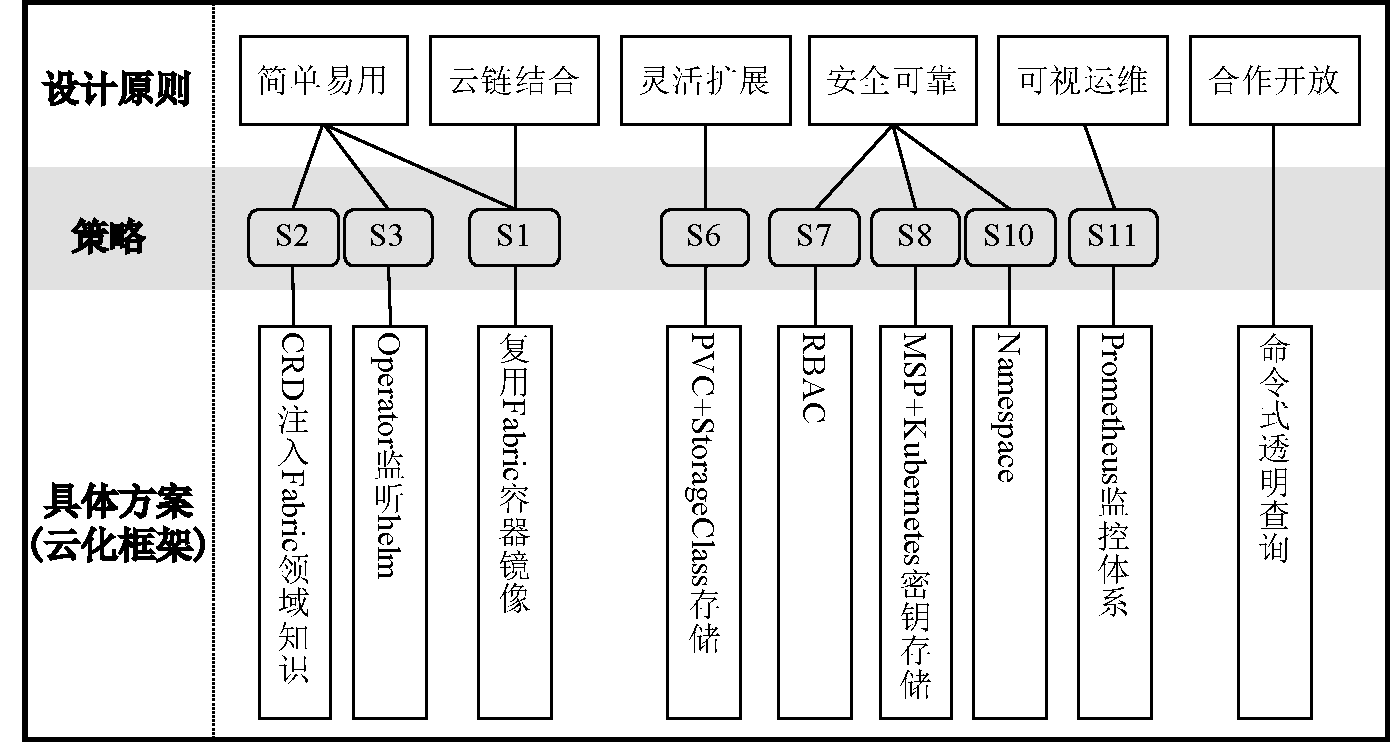
\includegraphics[width=1.0\textwidth]{FIGs/chapter3/policy_characteristics.pdf} %中括号中的参数是设置图片充满文档的大小,你也可以使用小数来缩小图片的尺寸。
    \caption{策略集应用} %caption是用来给图片加上图题的
    \label{policy_set_application} %这是添加标签,方便在文章中引用图片。
\end{figure}%figure环境


\section{本章小结}

本章为了解Kubernetes operator如何云化传统领域并对质量属性赋能, 首先详细介绍了快速评审的过程并得到基于Kubernetes operator云化策略集;其次, 本章重点介绍了基于Hyperledger Fabric的区块链云化框架所应满足的6条设计原则; 最后结合Fabric网络特性以及区块链云化框架设计原则对上述策略集进行筛选, 形成了基于Hyperledger Fabric的区块链云化框架的9个核心策略实施方案。

\chapter{智能合约微服务化开发运维方法}

本章首先详细分析智能合约开发运维过程中遇到的挑战, 并对比智能合约与微服务架构在设计原则上的相似性。基于这两者的相似性, 本章阐述了智能合约微服务化改造过程以及智能合约微服务化开发运维流程。最后, 本章介绍该方法的原型工具并对所提方法进行评估。

\section{研究目的}

区块链具有分布式、不可篡改、去中心化、历史可追溯等特点。自以太坊白皮书与黄皮书发布以来,智能合约被描述为图灵完备的、部署于区块链网络中的合同条款代码。图灵完备意味着智能合约可以执行复杂逻辑, 部署于区块链网络意味着传统的合同条款可以进入到实体计算机中,并在区块链网络去中心化、不可伪造、不可篡改的特性下执行。智能合约的引入有效的将上述特点落地到应用中。然而当前业界缺少促进去中心化应用价值交付的有效手段。具体地:

(1) 研究的重点是利用区块链技术特性应用在不同领域\cite{leka2019systematic}, 应用区块链技术,很大程度上就是利用区块链编写智能合约\cite{sun2018technology}。目前去中心化应用纷纷从概念验证阶段转化为工程化实践阶段。然而,智能合约的开发属全新的开发领域, 业界没有形成标准的开发流程。教育领域实践经验少\cite{yang2017application},使用门槛高。

(2) 当前业界对于智能合约的部署研究探索较少, 缺乏提高部署效率、缩短产品交付周期的有效工具与框架\cite{rodler2018sereum}。智能合约的部署通常采用的纯手工或脚本方式\cite{tiansong2019design}\cite{bumblauskas2020blockchain}, 消耗大量的时间成本。由于智能合约的不可修改性, 一旦区块链上的智能合约出现漏洞, 只能升级智能合约。另一方面,集成开发环境(Integrated Development Environment,简称IDE)对错误信息的支持差, HF工程师调试智能合约困难, 他们开发无漏洞智能合约具有挑战性。部署升级效率的低下使得无法及时更新链上存在漏洞的智能合约, 这些漏洞一旦被利用就会给客户带来财产损失, 动摇客户对智能合约的信心\cite{han2019security}。

(3) 此外,当前系统缺乏一套涵盖不同层面的标准方法来监控区块链系统\cite{li2020exploring},尤其是智能合约层面。业务逻辑中的请求、交易涉及多个智能合约, 这些智能合约通常由多个团队开发。当出现问题或者性能不佳的时候, 不仅执行过程无法中断而且缺乏错误日志, 这使得开发人员很难从错综复杂的服务调用网络中找到问题根源,故障难以检测、定位和修复。智能合约与共识节点耦合, 对于智能合约的运行状态、消耗物理资源的情况现阶段不可知。

综上, 智能合约学习使用门槛高、部署效率低、监控标准不完善, 严重限制区块链技术的推广使用和大规模落地。目前,亟需一体化、自动化的解决方案。随着DevOps理念的兴起, DevOps与微服务架构以其快速响应需求变更、持续部署、持续交付、持续监控等特点逐步取代单体架构。DevOps强调使用自动化工具来更快、更频繁地交付更稳定的软件。经过不断发展, 支撑微服务开发运维的自动化工具不断增多, 而这种自动化工具与能力正是智能合约开发和运维过程所欠缺的。为此, 本节提出一种智能合约微服务化开发运维方法。在该方法中, 首先进行智能合约微服务化改造, 经改造后的智能合约能够利用各种成熟的自动化工具支撑其开发运维工作。该方法扩充了智能合约开发运维工具库, 提升了智能合约开发运维的自动化水平, 最终能够提高去中心化应用的价值交付能力。本章的智能合约微服务化开发运维方法已经公开发表于国内高水平期刊《软件学报》。

\section{设计原则}

在智能合约微服务化开发运维方法之前, 需要考虑两者在设计原则上的相似性, 只有这两者在设计原则上相似才有可能进行智能合约微服务化改造。

微服务架构提倡将单一应用程序根据业务垂直划分成一组相互独立的小服务, 服务之间相互协调、互相配合, 为用户提供最终价值。每个服务运行在其独立的进程中, 服务和服务之间采用轻量级的通信机制相互沟通。每个服务都围绕着具体的业务进行构建, 并且能够被独立的部署到生产环境、类生产环境等, 这些服务可以使用不同的编程语言进行开发, 可以自由根据业务需求进行横向扩展。与此同时, 这些微服务分配给不同的团队进行开发维护, 做到对整个应用程序以及团队的解耦, 由于微服务的生命周期由小而精的团队全权负责, 它们更易维护且容错能力更强, 单独微服务的宕机不会影响破坏整个系统。

另一方面, 智能合约作为运行在区块链上的计算机程序, 极大丰富了区块链的功能, 使得区块链不仅仅是分布式账本, 并且能够完成一定程度的业务能力。在区块链出现之前, 信任的建立是基于诚信的中心化组织和个人。在区块链网络中没有中心化的记账机构, 其以密码学为基础, 所有的分布式节点执行共识机制来保障分布式账本不可伪造与不可篡改的特性, 所以用户可以信任区块链系统的数据。智能合约可以执行任何类型的计算, 由区块链驱动将会要求双方遵守他们的承诺并且智能合约永久储存且公开化, 这使得区块链从数据可信达到了业务可信。 如表\ref{Microservices_and_Smart_contract_Design_Principle}所示, 微服务与智能合约在设计原则上具有许多相似性\cite{weber2018blockchain}。

智能合约能够根据业务需求定义良好的边界。在边界内, 每个智能合约要求单一职责, 专注于自己的需求目标并且要完美的完成目标。但是, 目前智能合约在自动化、灵活性等方面还有很多欠缺, 因此如果将智能合约进行微服务化, 就能够借助微服务领域成熟的流程与技术规范智能合约的开发运维工作, 促进去中心化应用的价值交付流程。

{\footnotesize
\begin{longtable}[h]{m{100pt} m{100pt} m{150pt}}
    \caption[智能合约与微服务设计原则]{智能合约与微服务设计原则\cite{weber2018blockchain}} \label{Microservices_and_Smart_contract_Design_Principle} \\
        \toprule  
        \textbf{微服务设计原则}&\textbf{是否适用智能合约}&\textbf{理由} \\
        \hline
        小而精, 专注于功能 & 适用 & 每个智能合约都应该关注做很少的事情, 但要把这些做好  \\

        职责分离 & 适用 & 智能合约通常范围有限并负有全部责任 \\

        全栈 & 部分适用 & 根据上下文, 全栈或拆分智能合约可能是更好的选择 \\

        独立更新, 无需停机 & 部分适用 & 更新可以是独立的, 但依赖于治理, 这是对智能合约的信任来源之一 \\

        无状态 & 很少适用 & 典型的合同带有状态\\
        \bottomrule
    \end{longtable}
}

\section{智能合约微服务化改造}\label{section: smart_contract_micro}

本节探寻如何利用微服务思想改造智能合约, 使改造后的智能合约能够有效利用传统自动化工具支撑其开发运维工作。由于微服务的设计原则在很大程度上可以适用于智能合约, 这是本节能进行智能合约微服务化改造的基础。SpringBoot\footnotemark[1]\footnotetext[1]{\href{https://spring.io/projects/spring-boot}{SpringBoot}}是开发微服务的常用框架, 当前部署SpringBoot制品主要有以下两种方式:

\begin{itemize}[itemindent=2em]
    \item Jar包: 开发人员直接将编写好的Jar包以命令的方式运行在环境中的某端口上, 并对外暴露服务;

    \item 镜像发布: 开发人员将编写好的软件制品打包成Docker镜像, 打包好的镜像不仅可以直接运行并暴露端口对外服务, 而且可以托管于Kubernetes发布服务。托管于Kubernetes中的流程如图\ref{deploy_micro_by_container}所示。

\end{itemize}

\begin{figure}[h] %figure环境,h默认参数是可以浮动,不是固定在当前位置。如果要不浮动,你就可以使用大写float宏包的H参数,固定图片在当前位置,禁止浮动。
    \centering %使图片居中显示
    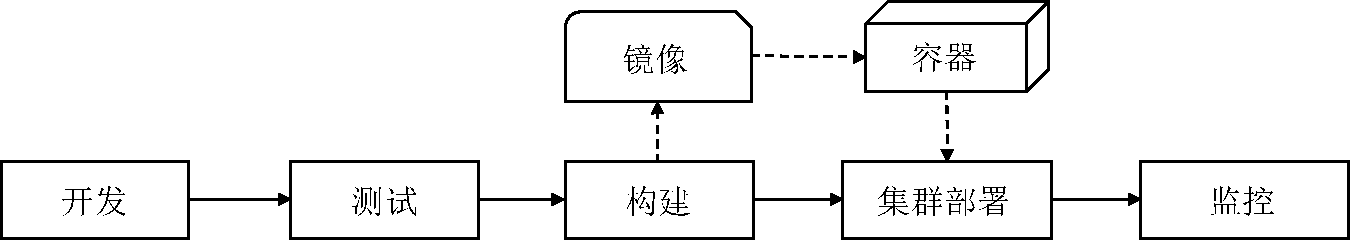
\includegraphics[width=1.0\textwidth]{FIGs/chapter4/deploy_micro_by_container.pdf} %中括号中的参数是设置图片充满文档的大小,你也可以使用小数来缩小图片的尺寸。
    \caption{镜像方式发布微服务流程} %caption是用来给图片加上图题的
    \label{deploy_micro_by_container} %这是添加标签,方便在文章中引用图片。
\end{figure}%figure环境

由于当前智能合约与区块链节点之间是强耦合的关系, 这使得我们很难利用现有工具单独对智能合约进行独立开发、测试、部署、运维。因此, 
本节进行的智能合约微服务化改造流程如图\ref{microservice_for_sc}所示。

\begin{figure}[h] %figure环境,h默认参数是可以浮动,不是固定在当前位置。如果要不浮动,你就可以使用大写float宏包的H参数,固定图片在当前位置,禁止浮动。
    \centering %使图片居中显示
    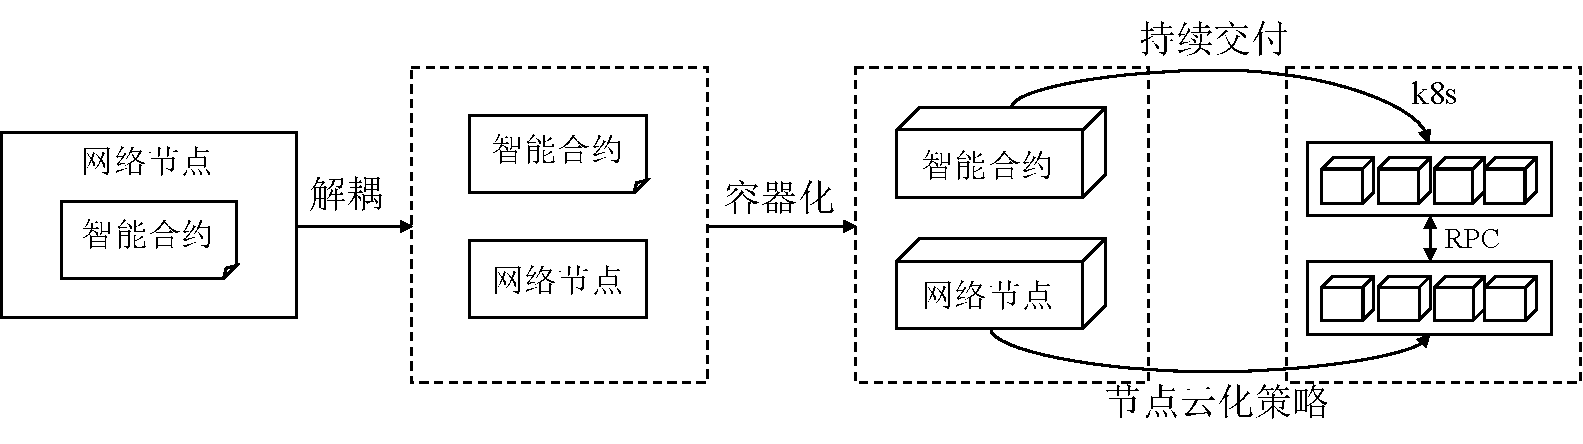
\includegraphics[width=1.0\textwidth]{FIGs/chapter4/microservice_for_sc.pdf} %中括号中的参数是设置图片充满文档的大小,你也可以使用小数来缩小图片的尺寸。
    \caption{智能合约微服务化改造流程} %caption是用来给图片加上图题的
    \label{microservice_for_sc} %这是添加标签,方便在文章中引用图片。
\end{figure}%figure环境

\textbf{(1) 运行环境}

智能合约微服务化改造的目的是解耦, 让智能合约更容易拓展、更富有弹性。在传统的链码安装与实例化的方式中, 链码的构建和运行是HF节点的一部分, 链码和节点之间的耦合度较高, 不具有可复用性。解耦后的智能合约更加专注于自身功能, 不需要关心账本数据的一致性、网络的安全性等问题。解耦后, 需要给智能合约提供容器环境使其可以运行。可以说, 容器化是智能合约与共识节点解耦后平稳运行的基础, 是智能合约微服务化的有效手段。本节将智能合约与网络节点解耦后具备以下优势:

\begin{itemize}[itemindent=2em]
    \item 单一职责: 职责愈加明确, 每个智能合约容器只需要完成自己特定的功能。独立的智能合约能够有效利用现有自动化工具完成持续交付; 

    \item 高融入性\footnotemark[1]\footnotetext[1]{\href{http://pss-system.cnipa.gov.cn/sipopublicsearch/patentsearch/showViewList-jumpToView.shtml}{发明专利: 一种建立智能合约微服务化的方法}}: 智能合约将服务封装成API, 用户可直接将智能合约安插在自己的业务逻辑中;

    \item 高可用性: 利用Kubernetes本身对于高可用性的保障,只需要在Kubernetes层面进行简单的配置(例如Replica、QoS、HPA等),不必针对区块链层面专门进行高可用策略配置;

    \item 高可扩展性: 智能合约进行容器化编排后, 只需要将自己的服务暴露给其他节点及应用。当智能合约需求发生变更时, 只需向集群内部增加新变更的智能合约容器即可。
\end{itemize}


\textbf{(2) 通信机制}

智能合约解耦后需要为智能合约与网络节点提供良好的通信机制, 只有合理有效的通信才能保证智能合约正确的运行。

如表\ref{two_communication}所示, 服务间通信的方式主要有两种, 分别是远程过程调用(Remote Procedure Call, 简称RPC)和表述性状态转移(Representational State Transfer, 简称REST)。这两种方式各有利弊, 存在不同的使用场景。本节的智能合约微服务化改造为保证区块链网络的性能选择RPC的通信方式。

{\footnotesize
\begin{longtable}[h]{m{50pt} m{120pt} m{120pt}}
    \caption[通信机制对比]{通信机制对比} \label{two_communication} \\
        \toprule  
        \textbf{}&\textbf{RPC}&\textbf{REST} \\
        \hline
        场景 & 适用于内部的函数方法调用 & 适用于外部资源接口  \\

        优点 & 性能表现出色 & 便于开发人员理解、调试 \\

        缺点 & 与代码耦合度强, 不方便理解 & 性能表现较差 \\
        \bottomrule
    \end{longtable}
}

\textbf{(3) 持续交付}

持续集成(Continuous Integration, 简称CI)是一种软件开发实践, 团队成员经常集成他们的工作, 通常每个人至少每天都进行集成。每个集成都由自动化的构建(包括测试)进行验证, 以尽可能快地检测集成错误\footnotemark[1]\footnotetext[1]{\href{https://moodle2019-20.ua.es/moodle/pluginfile.php/2228/mod_resource/content/2/martin-fowler-continuous-integration.pdf}{Martin Fowler.Continuous Integration.}}。持续交付(Continuous Delivery, 简称CD)的关注点不在于源码而在于可交付物。

借鉴微服务持续交付的思想, 智能合约从编写完成后就要不断的集成交付。只有持续不断的交付才能持续验证智能合约与下层的区块链云化节点结合的功能完整性。当前, 可交付物从代码制品变为智能合约镜像, 借鉴现有的CI/CD工具(例如Jenkins、Travis CI等)帮助智能合约微服务化开发快速构建持续交付流水线, 可以实现:

\begin{itemize}[itemindent=2em]
    \item 基础设施自动化, 为智能合约微服务化开发降低了构建、部署、交付操作难度,减少集成交付过程中的时间开销;

    \item 频繁的构建升级智能合约, 更早的识别错误, 有效控制风险, 保证代码质量;

    \item 有效的帮助团队成员之间的协作, 促进代码共享, 团队中每个人都能看到构建交付结果。
\end{itemize}


\section{智能合约微服务化开发运维流程}\label{section: smart_contract_micro}

本节智能合约微服务化提供一套从需求、开发、构建、测试、部署到监控的流程指导, 如图\ref{sc_develop}展示了智能合约微服务化开发运维流程以促进智能合约价值交付过程。该图展示的是在已经搭建好的区块链云化网络中, 使用现有自动化工具无侵入的支撑智能合约完整生命周期。

\begin{figure}[h] %figure环境,h默认参数是可以浮动,不是固定在当前位置。如果要不浮动,你就可以使用大写float宏包的H参数,固定图片在当前位置,禁止浮动。
    \centering %使图片居中显示
    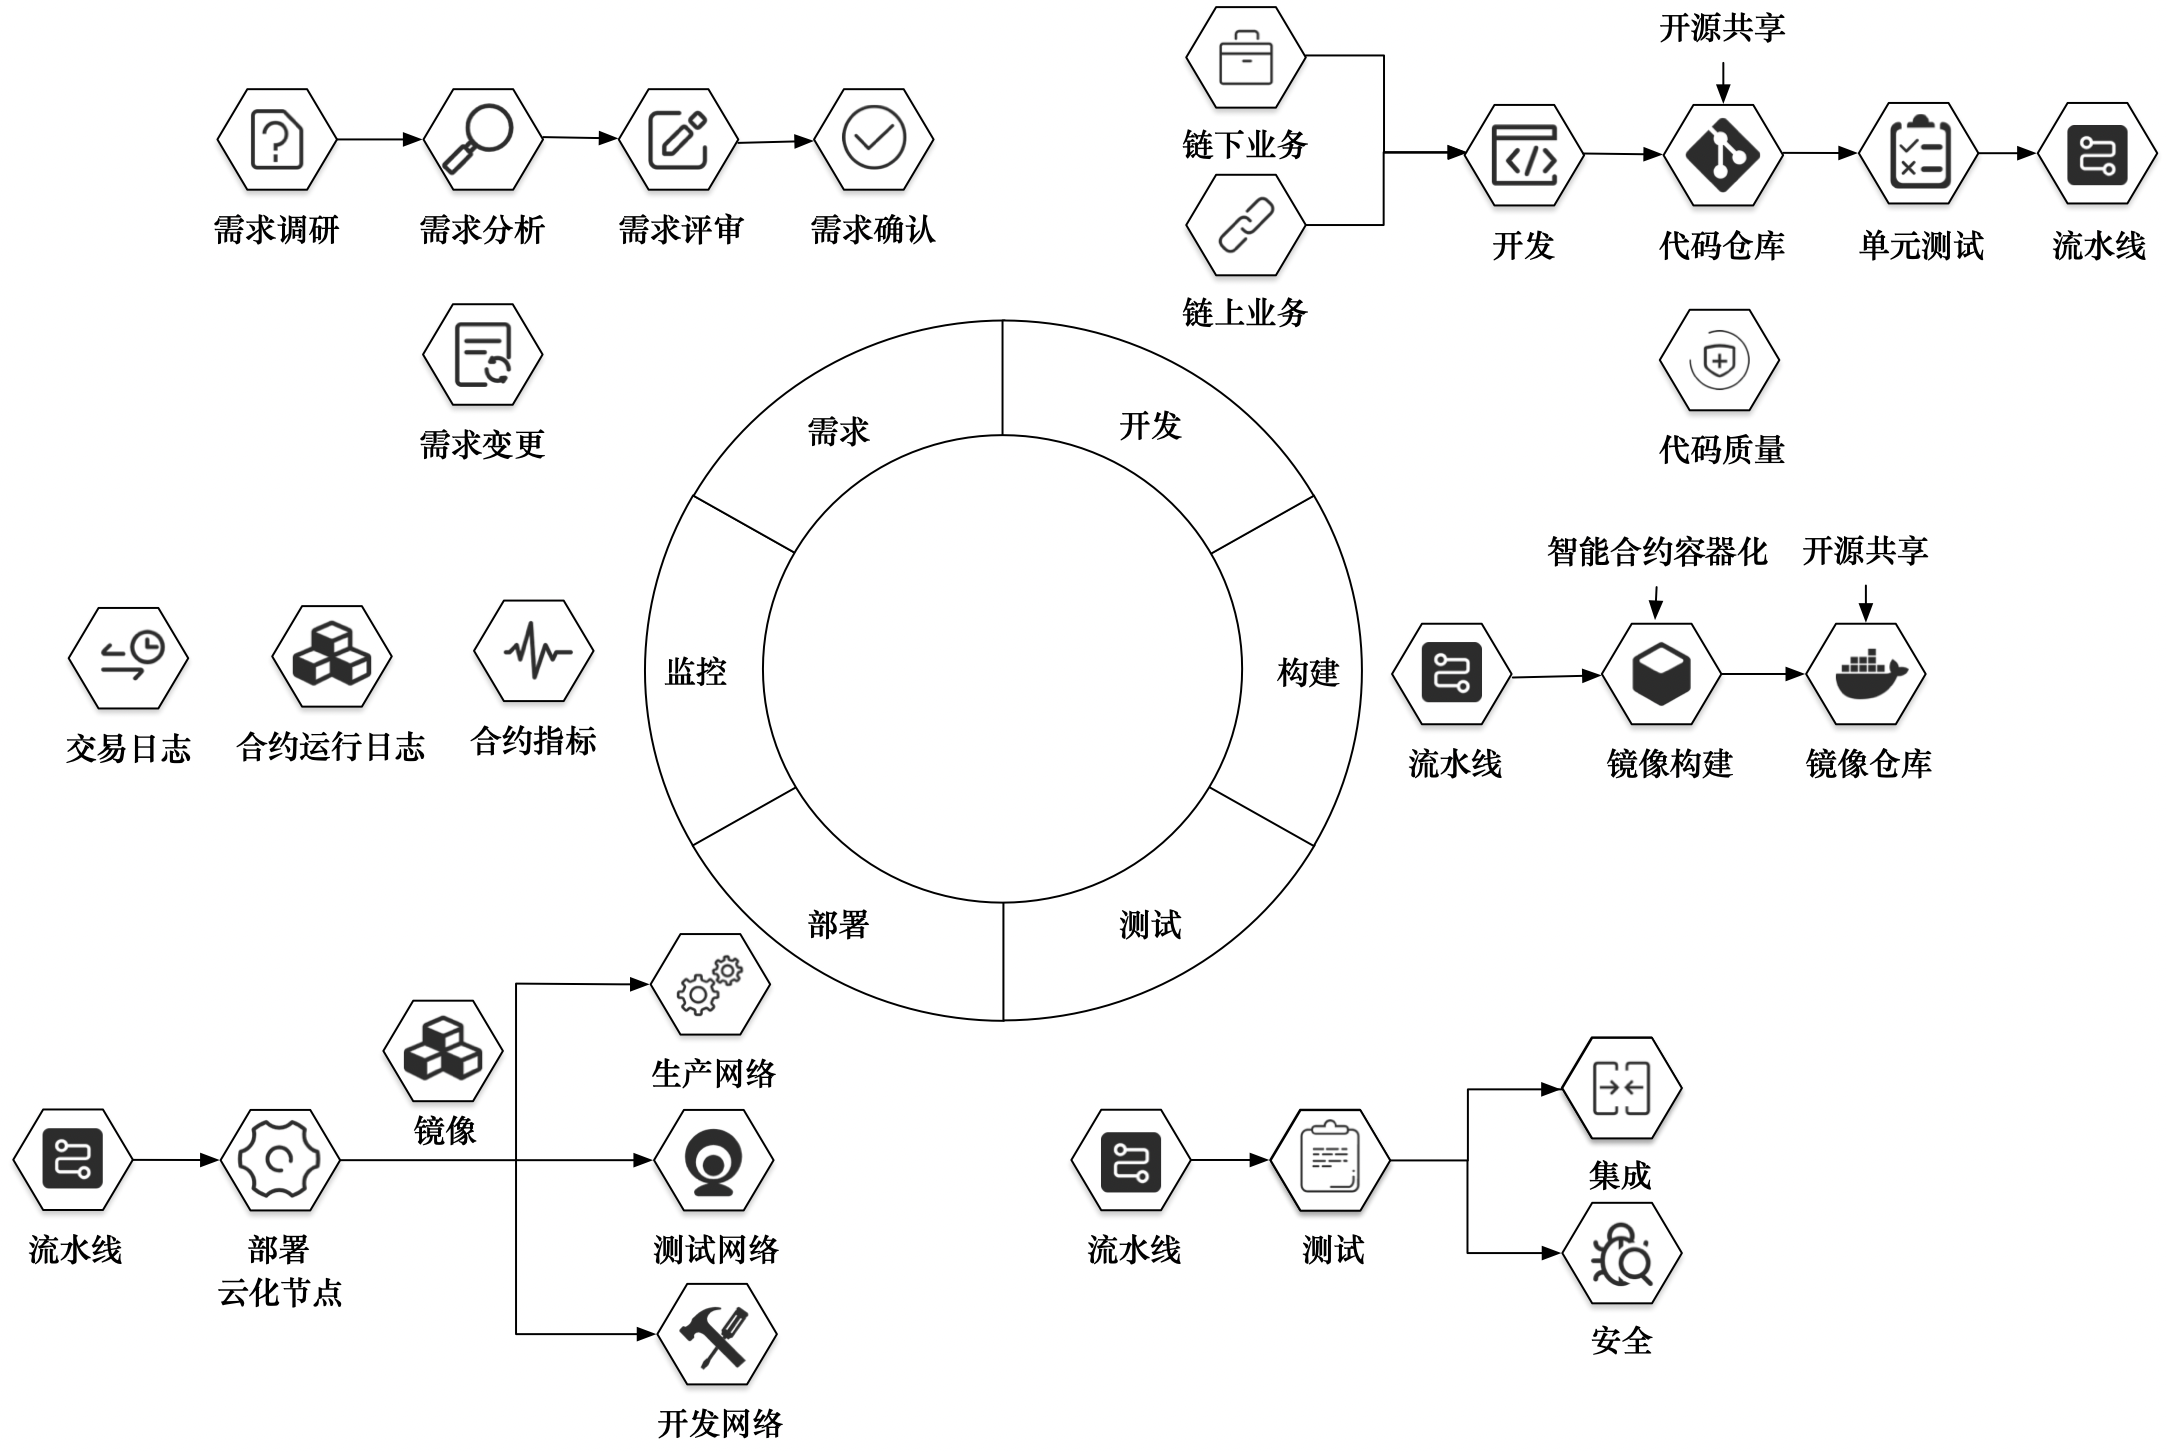
\includegraphics[width=1.0\textwidth]{FIGs/chapter4/process.png} %中括号中的参数是设置图片充满文档的大小,你也可以使用小数来缩小图片的尺寸。
    \caption{智能合约微服务化开发运维流程} %caption是用来给图片加上图题的
    \label{sc_develop} %这是添加标签,方便在文章中引用图片。
\end{figure}%figure环境

\textbf{(1) 需求}

区块链网络是一个典型的分布式网络, 在理论计算机科学中, Eric Brewer提出CAP定理\footnotemark[1]\footnotetext[1]{\href{https://en.wikipedia.org/wiki/CAP_theorem}{CAP Theorem}},分布式数据存储系统中只能同时满足以下三个中的两个:

\begin{itemize}[itemindent=2em]
    \item 一致性(Consistency): 所有节点数据一致性更新;

    \item 可用性(Availability): 系统是否还能在正常时间内响应用户的请求;

    \item 分区可用性(Partition Tolerance): 尽管节点之间的网络丢弃(或延迟)任意数量的消息, 系统仍将继续运行.

\end{itemize}

分布式系统必须满足分区可用性, 即某个节点宕机不会影响其他节点的正常工作, 达到高可靠性。在区块链系统中, 要求所有节点共同维护相同的账本, 所以必须满足一致性原则。在满足上述两个原则的条件下就要牺牲可用性, 系统的响应时间则会变慢。

将一个大的复杂问题,变成多个小问题解决,体现了微服务架构的分而治之的思想。合理的微服务划分是微服务架构成功与否的关键, 但是微服务架构是手段而不是最终的目的。智能合约微服务化改造的最终目的是解耦, 以业务为根本出发点进行抽象划分。为了使去中心化应用具备良好的响应性能,所以在需求分析阶段智能合约需要额外考虑微服务架构在数据处理响应时间方面的区别。区块链的新数据要经过多个节点消耗大量的计算资源才会产生且数据会有多处冗余的备份, 对于大流量数据与实时性要求比较高的数据并不建议使用链上智能合约代码处理, 仅将需要达成共识的数据上链即可。


\textbf{(2) 开发}

当链上业务代码编写完成后托管于代码仓库, 由于现如今智能合约很少开源, 本文提倡以代码库或镜像库的形式分享有用且经过市场检验的智能合约, 促进业界交流, 减少重复开发。开发过程中, 智能合约与其他业务代码隔离, 彼此之间可以使用不同的编程语言。将智能合约开源, 帮助工程师更快了解智能合约内部的工作原理。开发的代码仓库可以对接CI/CD工具, 做到合并代码后自动提交流水线交付。


\textbf{(3) 构建}

智能合约的开发和升级过程都比较繁琐, 所以智能合约的手动部署、版本更迭以及升级过程都容易出错, 这有可能会导致系统漏洞, 甚至升级失败, 造成数据和经济损失。利用已有CI/CD工具实现基础设施自动化,利用容器化工具(如Docker)打包编写完成的智能合约, 衔接测试和部署。同样,将合格的智能合约镜像开源可以方便其他开发者直接部署于自己的区块链网络。

\textbf{(4) 测试}

常见的智能合约漏洞包括重入攻击、事务顺序依赖、时间戳依赖、处理异常、整型溢出等。尽管业界已有各种理论与工具\cite{luu2016making},但自动化程度较低。本文利用持续集成工具提升智能合约测试的自动化水平, 将“可插拔”、“开箱即用”的测试策略配置进入持续交付流水线, 以便在智能合约上链前对其进行全方位测试。

\textbf{(5) 部署}

本文提倡从一开始不断的集成, 将拆分后的智能合约以及区块链共识节点组合起来。每个过程都由自动化的构建(包括测试)进行验证, 以尽可能快地检测集成的错误。智能合约可交付镜像可以在开发、测试、生产环境之间无障碍流通, 打破三者之间的隔阂。开发完成的镜像可以直接交给测试网络测试, 测试完成的镜像可以直接在生产环境中部署。

\textbf{(6) 监控}

在智能合约微服务运行时采用已有监控工具全面采集智能合约容器以及下层区块链云化网络节点的性能指标数据,提供一个标准和定制的性能框架。该框架可以集成数据异常检测、报警、智能决策分析以及可视化。常见的监控指标有:
\begin{itemize}[itemindent=2em]
    \item  响应时间: 每个事务的响应时间,包括平均响应时间、最大响应时间和最小响应时间;

    \item 吞吐量: 每秒成功事务的数量;

    \item 成功率: 成功交易的数量与全部交易数量的比值;

    \item 资源消耗: CPU、内存、磁盘和网络I/O等。

\end{itemize}

\section{原型工具与方法评估}\label{section: smart_contract_microservice_test}

由于本章的智能合约微服务化开发运维方法已经公开发表, 故本节将简要描述基于智能合约微服务化开发运维方法的原型工具Mictract核心工作原理以及智能合约微服务化开发运维方法的评估过程。

如图\ref{mictract}所示, Mictract\footnotemark[1]\footnotetext[1]{\href{https://github.com/doporg/Mictract}{Java for Mictract}}\footnotemark[2]\footnotetext[2]{\href{https://github.com/doporg/Mictract-go-server}{Go for Mictract}}作为传统BaaS平台能够为构建区块链应用程序的人或组织提供第三方区块链服务, 允许用户构建、托管、运行、监控自己的区块链应用。Mictract的核心优势是具备BaaS平台基本功能的前提下, 屏蔽了底层方法原理与工具, 形成了支撑智能合约开发运维的工具链。值得注意的是, Mictract搭建的下层区块链网络与传统BaaS平台类似, 只是简单的将区块链网络迁移上云。因此, Mictract在下层网络节点云化方面存在一定的不足, 需要整合区块链节点云化方案形成完整的区块链云化框架。

\begin{figure}[h] %figure环境,h默认参数是可以浮动,不是固定在当前位置。如果要不浮动,你就可以使用大写float宏包的H参数,固定图片在当前位置,禁止浮动。
    \centering %使图片居中显示
    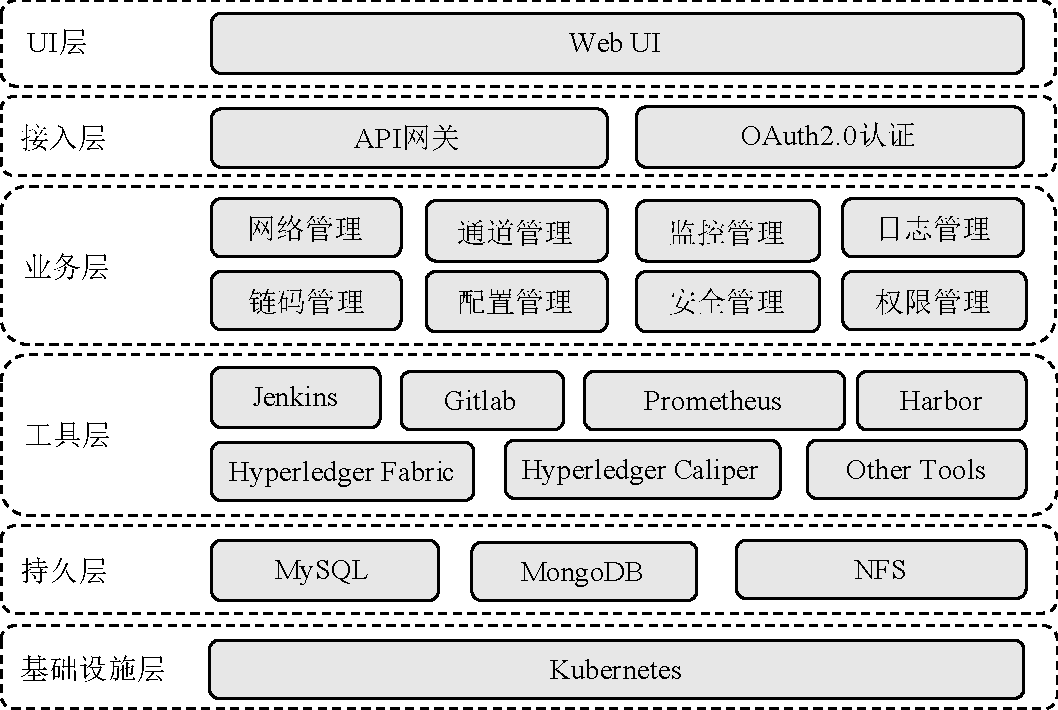
\includegraphics[width=0.9\textwidth]{FIGs/chapter4/mictract.pdf} %中括号中的参数是设置图片充满文档的大小,你也可以使用小数来缩小图片的尺寸。
    \caption{Mictract架构图} %caption是用来给图片加上图题的
    \label{mictract} %这是添加标签,方便在文章中引用图片。
\end{figure}%figure环境

将官方HF的链码打包成Docker镜像并将这些镜像部署于Kubernetes是智能合约微服务化的基础也是阻碍智能合约微服务化的主要问题。HF 2.0引入了链码新生命周期, 工程师通过新生命周期命令可以打包新类型链码包, 并生成一个链码包的packageID。原型工具利用伪代码\ref{cc_dockerfile}将链码打包成Docker镜像。当需要部署链码时, 利用伪代码\ref{code4}配置链码的部署文件,拉取链码镜像并为其配置环境变量, 最终生成相应的Kubernetes Pod容器作为独立的运行单元。除了对上述镜像及Deployment的改造外, Mictract在核心部署环节还存在三个难点:

\begin{itemize}[itemindent=2em]
    \item  Kubernetes部署Deployment时, Kubernetes在非人为指定下会选择出集群中适合运行当前Pod资源的一个节点, 这种资源调度策略很可能使Pod与证书文件、初始区块或者通道文件处于不同节点, 所以采用NFS文件服务器的方式将上述配置文件共享;

    \item Mictract将packageID等环境变量和共享的配置文件以Deployment容器变量的形式传入;

    \item 将Peer声明为外部链码构建形式并为其传入外部链码构建器启动器。同时, 将Peer节点生成外部链码标识符传入外部链码的Deployment容器。
\end{itemize}

\begin{algorithm}[!htbp]
    \floatname{algorithm}{\footnotesize 伪代码}
    \caption{\footnotesize 智能合约Dockerfile伪代码}
    \label{cc_dockerfile}
    {\footnotesize
    \begin{algorithmic}
        \renewcommand{\algorithmicrequire}{ \textbf{Input:}}
        \REQUIRE  
        智能合约代码
        \renewcommand{\algorithmicensure}{\textbf{Output:}}
        \ENSURE
        暴露端口提供服务

        \STATE{FROM <base-image:tage>}
        \STATE{COPY <src> <dest>}
        \STATE{WORKDIR <dest> }
        \STATE{RUN <build-command>}
        \STATE{EXPOSE <port>}
        \STATE{CMD <run-command>}
    \end{algorithmic}
    }
\end{algorithm}

\begin{algorithm}[!htbp]
    \floatname{algorithm}{\footnotesize 伪代码}
    \caption{\footnotesize 智能合约 Deployment伪代码}
    \label{code4}
    {\footnotesize
    \begin{algorithmic}
        \renewcommand{\algorithmicrequire}{ \textbf{Input:}}
        \REQUIRE  
        链码镜像地址, 命名空间, 链码包packageID
        \renewcommand{\algorithmicensure}{\textbf{Output:}}
        \ENSURE
        暴露端口提供服务

        \STATE{namespace <namespace>}
        \STATE{containers: image <image-uri>}
        \STATE{image: imagePullPolicy <IFNotPresent>}
        \STATE{env: CHAINCODE-PACKAGEID <packageID>}
        \STATE{env: CHAINCODE-ADDRESS <address>}
        \STATE{container: port <port>}
    \end{algorithmic}
    }
\end{algorithm}

在测试方面, Mictract提供对Go语言编写链码的测试, 其借鉴HF的 MockStub类完成账本初始化工作, 采用MockStub类单元测试以及性能测试, 利用pprof\footnotemark[1]\footnotetext[1]{\href{https://github.com/google/pprof}{go pprof github地址}}完成性能剖析工作; 在智能合约监控层面, Mictract提供智能合约资源消耗以及交易过程监控两个方面的监控。

为了验证本节提出的智能合约微服务化开发运维方法的可行性与部署效率, 本节选取了官方链码asset进行案例研究, 使用智能合约微服务化开发运维方法对asset进行托管、运行、监控。可行性是本文首要关心的问题, 智能合约微服务化开发运维方法需保证智能合约运行无误。为此本文将官方asset链码进行微服务化改造, 验证其是否满足预期功能。操作过程如下表\ref{operator_chaincode}所示, 该表为表明智能合约微服务化开发运维方法确保智能合约正确运行, 并不是为了展示asset链码本身的功能, 故未进行全部功能的调用。结果表明, 智能合约微服务化改造满足预期, 可以保证智能合约运行的正确。

目前, 缺乏智能合约微服务化的有效评估指标。由于智能合约微服务化开发运维方法的目的是利用已有的成熟工具快速部署、操作、监控智能合约, 以此来提升智能合约开发运维自动化水平, 故本文选取部署效率作为分析指标。表\ref{experimental_results_of_smart contract_micro_service}展示了采用官方脚本方式以及智能合约微服务化开发运维方法搭建、部署不同网络规模所消耗的时间。由于Peer节点的数量、组织的数量以及通信效率的影响, 同一规格的网络部署时间可能会略有差别。在环境完备且中间不出现Bug的前提下采用脚本方式比智能合约微服务化开发运维方法平均多使用225.6秒。该方法整合进入面向Hyperledger Fabric的区块链云化框架后与官方BaaS平台Cello针对链码部署效率的对比情况详见第\ref{section: tool_comparison}节。

{\footnotesize
\begin{longtable}[h]{l m{90pt} m{210pt} l}
    \caption[操作链码实例]{操作链码实例} \label{operator_chaincode}\\
        \toprule  
        \textbf{步骤}&\textbf{操作}&\textbf{预期结果}&\textbf{实际}\\
        \hline
        step1 & InitLedger() & txid=<TXID> & 通过 \\
        \hline
        step2 & GetAllAssets() & [\{“Key”:“asset1”,“Record”:\{“ID”:“asset1”,“color”:“blue”,“size”:5,“owner”:“Tomoko”,“appraisedValue”:300\}\}, 
        \newline \{“Key”:“asset2”,“Record”:\{“ID”:“asset2”,“color”:“red”, “size”:5,“owner”:“Brad”,“appraisedValue”:400\}\}] & 通过 \\
        \hline
        step3 & ReadAsset(“asset1”) & \{“ID”:“asset1”,“color”:“blue”,“size”:5,“owner”:“Tomoko”,
        "appraisedValue":300\} txid=<TXID> & 通过 \\
        \hline
        step4 & TransferAsset(“asset1”, “Brad”) & Tomoko txid=<TXID>   & 通过 \\
        \hline
        step5 & ReadAsset(“asset1”) & \{“ID”:“asset1”,“color”:“blue”,“size”:5,“owner”:“Brad”,
        "appraisedValue":300\} txid=<TXID>  & 通过 \\
        \bottomrule
        
    \end{longtable} 
}

{\footnotesize
\begin{longtable}[h]{ccccc}
    \caption[部署效率对比(单位: 秒(s))]{部署效率对比(单位: 秒(s))} \label{experimental_results_of_smart contract_micro_service}\\
        \toprule  
        \textbf{总Peer数}&\textbf{总Orderer数}&\textbf{组织数量}&\textbf{脚本方式}&\textbf{智能合约微服务化方法}\\
        \hline
        2 & 2 & 2 & 342 & 136\\
        4 & 3 & 2 & 440 & 185\\
        2 & 3 & 2 & 358 & 146\\
        3 & 4 & 3 & 483 & 202\\
        1 & 2 & 1 & 306 & 132\\
        \bottomrule
    \end{longtable} 
}

\section{本章小结}

本章首先分析了智能合约开发运维过程中的挑战, 并分析了智能合约与微服务架构在设计原则上的相似性, 结果表明智能合约与微服务都具备相似的特性。基于这种相似性, 本章随后阐述了智能合约微服务化改造过程, 包含核心的解耦思想、运行环境以及通信机制, 然后提出了智能合约微服务化开发运维流程。最后, 本章介绍了方法的原型工具并对所提方法进行了可行性与部署效率的评估。

\chapter{面向Hyperledger Fabric的区块链云化框架}

本章首先阐述面向Hyperledger Fabric的区块链云化框架的原理、流程以及输入、处理单元和输出, 随后给出了基于该框架的原型工具的需求分析、设计以及相关实现。

\section{面向Hyperledger Fabric的区块链云化框架}\label{section: framework}

区块链的成熟以及BaaS的市场规模不断扩大促进了去中心应用的落地, 同时对云原生服务市场也促进明显。云的开放、动态可伸缩的能力成为了去中心化应用落地的最佳载体。结合第\ref{section: policy_set_application}节所得的策略具体实施方案和第\ref{section: smart_contract_micro}节的智能合约微服务化开发运维流程, 本文提出了面向Hyperledger Fabric的区块链云化框架, 利用Kubernetes Operator方法将领域知识集成到Kubernetes API编排过程中\cite{henning2021reproducible}。Kubernetes API是云原生容器管理系统的大脑, 它是一个复杂的API, 具有多个层与各种资源\cite{Yilmaz2021}。由于已经介绍了Mictract对于智能合约微服务化开发运维流程的支持, 故本章侧重介绍区块链网络节点利用BaaS计算资源层Kubernetes的计算资源、存储资源等资源实现节点云化。该框架能够提供完备的 去中心化应用开发能力同时提供隐式管理密码文件、按需配置调度Kubernetes资源, 解决HF生产部署效率、安全性、数据弹性等运营难题, 节约开发人员以及运维人员时间成本, 使得其更加专注于去中心化应用的逻辑。

Operator应该管理单一类型的应用程序, 遵循UNIX原则:只做一件事, 并把它做好\cite{d2020design}。本框架必须解决的首要任务是屏蔽HF及Kubernetes底层细节, 简化HF网络各节点的部署, 以及有效利用Kubernetes代码化、云化的管理基础设施, 所以本框架需要分别对Ca、Orderer、Peer三种不同的网络节点进行完整生命周期管理。同时, 本框架需要承接来自持续交付工具的链码安装部署任务, 所以也需要能够对链码进行监控管理。

如图\ref{framework}所示, 本框架的整体工作流程将分为几个步骤。首先, 将HF领域知识注入CRD, 这些属性包含HF网络中Ca、Orderer、Peer各节点以及链码所具备的功能、性能、监控等可插拔的基础属性。将CRD作为本框架的输入, 通过自定义命令完成静态CRD相关属性的配置。其次, Manager是本框架的处理单元, 其被设计成一个黑盒\cite{yu2020system}, 用户无需关心Manager的内部逻辑设计。 Manager自动生成部署的配置文件, 使用生成的配置文件并结合Helm可以轻松的将HF网络各节点部署进目标Kubernetes集群。部署成功后, Manager持续监控这些节点及其存储资源的状态。除此网络节点外, Manager还会持续监听来自持续交付工具所产生的部署链码任务以启动对应的链码容器。Manager根据持续监测结果调用Kubernetes及HF相关API将各节点及链码调整到期望状态以维持HF网络的稳定。最后, HF网络是本框架的输出, 除HF网络各节点基本Deployment、Service外, 本框架利用Istio基础设施层完成高性能、适应性和可用性\cite{li2019service}\cite{larsson2020impact}的TLS通信负载均衡; 采用原生Role、Secret、PVC等方式管理HF网络的权限、密码及存储。

\begin{figure}[h] %figure环境,h默认参数是可以浮动,不是固定在当前位置。如果要不浮动,你就可以使用大写float宏包的H参数,固定图片在当前位置,禁止浮动。
    \centering %使图片居中显示
    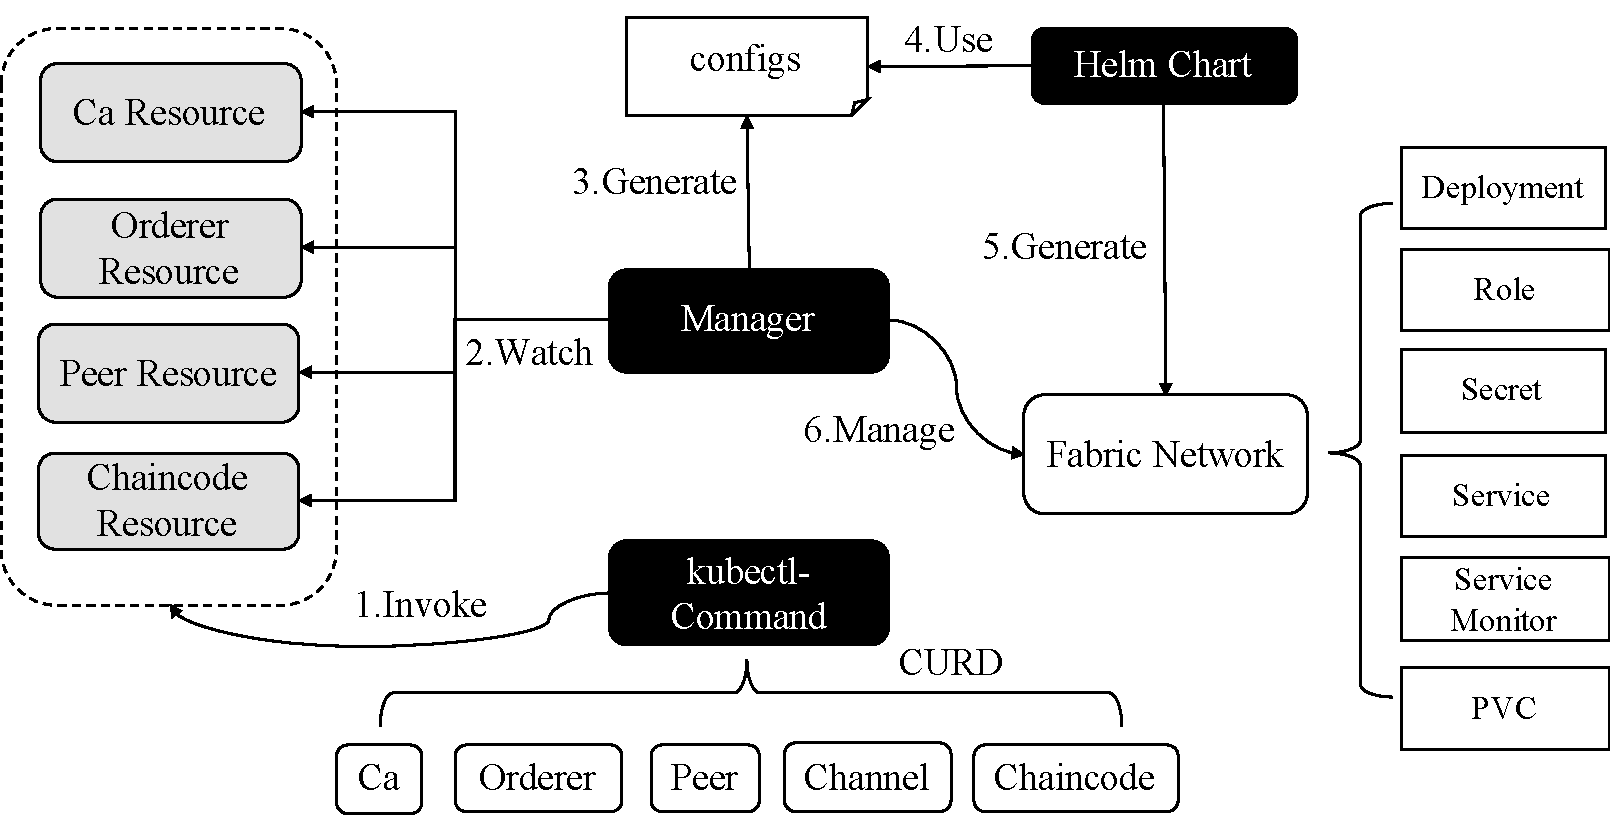
\includegraphics[width=1.0\textwidth]{FIGs/chapter5/framework.pdf} %中括号中的参数是设置图片充满文档的大小,你也可以使用小数来缩小图片的尺寸。
    \caption{面向Hyperledger Fabric的区块链云化框架} %caption是用来给图片加上图题的
    \label{framework} %这是添加标签,方便在文章中引用图片。
\end{figure}%figure环境

\subsection{Custom Resource Definition}\label{section: Custom_Resource_Definition}

虽然HF和Kubernetes形成了理想的匹配, 但许多HF网络管理员缺乏必要的Kubernetes专业知识, 集群管理员的区块链领域知识也相对匮乏。CRD则通过扩展Kubernetes API将具备领域知识的资源类型注入进Kubernetes集群中。Kubernetes提供了标准资源ConfigMap, 也可用于使配置数据项供应用程序使用, 但这两种针对不同的情况。ConfigMap擅长为Pod中运行的程序提供配置, 应用程序通常希望从Pod中读取此类配置, 例如文件或环境变量的值, 而不是从Kubernetes API中读取。CR由标准的Kubernetes客户端创建和访问, 遵守Kubernetes规范。通过Controller可以监控CR运行, 这些代码可以反过来创建、更新或删除其他集群对象, 甚至集群外的任意资源。

{\footnotesize
\begin{longtable}[h]{m{60pt}|m{100pt}|m{210pt}}
    \caption[CRD描述]{CRD描述} \label{crd_description} \\
        \hline   
        \textbf{CRD名称}&\textbf{属性}&\textbf{描述}\\
        \hline
        \multirow{8}*{\parbox[c]{60pt}{Ca Resource \\ Definition}}
        & CRLSizeLimit & 可接受证书撤销列表(Certificate Revocation List, 简称CRL)的大小限制 \\\cline{2-3}
        & TLS & 服务器侦听TLS端口以及证书等信息 \\\cline{2-3}
        & CA & 包含与证书颁发机构相关的信息 \\\cline{2-3}
        & Database & 用作数据存储 \\\cline{2-3}
        & CFG & 配置身份允许的错误密码尝试次数 \\\cline{2-3}
        & CSR & 控制根CA证书的创建, 如根CA证书的过期时间配置 \\\cline{2-3}
        & Registry & 部分控制fabric-ca服务器执行验证包含用户名和密码的注册和检索标识的属性名称、值的方式 \\\cline{2-3}
        & BCCSP & 用于选择要使用的加密库实现 \\\cline{2-3}
        \hline  
        \multirow{4}*{\parbox[c]{60pt}{Orderer \\ Resource \\ Definition}}
        & Genesis & 初始区块相关配置 \\\cline{2-3}
        & BootstrapMethod & 指定了获取引导块系统通道的方法 \\\cline{2-3}
        & ChannelParticipation & 通道管理对系统链码的依赖 \\\cline{2-3}
        & Secret & 包含Orderer数字签名以及与Ca通信所需的基本信息\\\cline{2-3}
        \hline 
        \multirow{7}*{\parbox[c]{60pt}{Peer Resource \\ Definition}}
        & Gossip & 确保Peer间通过Gossip协议来达到所有账本的最终一致性 \\\cline{2-3}
        & LevelDB/CouchDB & HF提供LevelDB与CouchDB用以保存HF账本信息, 用以灵活适应Peer不同数据库之间的转换 \\\cline{2-3}
        & CouchDBExporter & 采集CouchDB的监控数据 \\\cline{2-3}
        & ExternalChaincodeBuilder & 提供外部链码构建的能力 \\\cline{2-3}
        & Secret & 包含Peer的数字签名以及与Ca通信所需的基本信息\\\cline{2-3}
        & MSP & 所属的组织信息\\\cline{2-3}
        \hline 

        \multirow{3}*{\parbox[c]{60pt}{Chaincode \\ Resource \\ Definition}}
        & PackageID &  链码唯一标识符 \\\cline{2-3}
        & Secret &  包含用户的数字签名以及与Ca通信所需的基本信息 \\\cline{2-3}
        & Env &  包含链码所需要的环境变量信息 \\\cline{2-3}     
        \hline 
    \end{longtable} 
}

HF作为一种去中心化的多方信息对接的网络, 具有一套标准化的数据结构与接口。本框架基于HF网络各节点自身功能及配置\footnotemark[1]\footnotetext[1]{\href{https://github.com/hyperledger/fabric-ca/blob/main/cmd/fabric-ca-server/config.go}{Ca Config}}\footnotemark[2]\footnotetext[2]{\href{https://github.com/hyperledger/fabric/blob/main/sampleconfig/orderer.yaml}{Orderer Config}}\footnotemark[3]\footnotetext[3]{\href{https://github.com/hyperledger/fabric/blob/main/sampleconfig/core.yaml}{Peer Config}}设计三种HF静态资源类型以及一种链码动态资源类型作为输入(S2), 包括但不限于如表\ref{crd_description}所示的属性, 篇幅原因仅展示部分内容。额外的, 除上述针对不同网络节点的特殊属性外, 本框架为每个节点及链码提供如副本数、镜像、Hosts、日志、ServiceMonitor等基本属性维持HF网络的基本运行状态。


\subsection{Manager}

CR本身仅为特定应用程序提供声明式API的数据项的集合, Controller负责对CR的不同事件做出反馈, 管理CR的完整生命周期。

\begin{figure}[h] %figure环境,h默认参数是可以浮动,不是固定在当前位置。如果要不浮动,你就可以使用大写float宏包的H参数,固定图片在当前位置,禁止浮动。
    \centering %使图片居中显示
    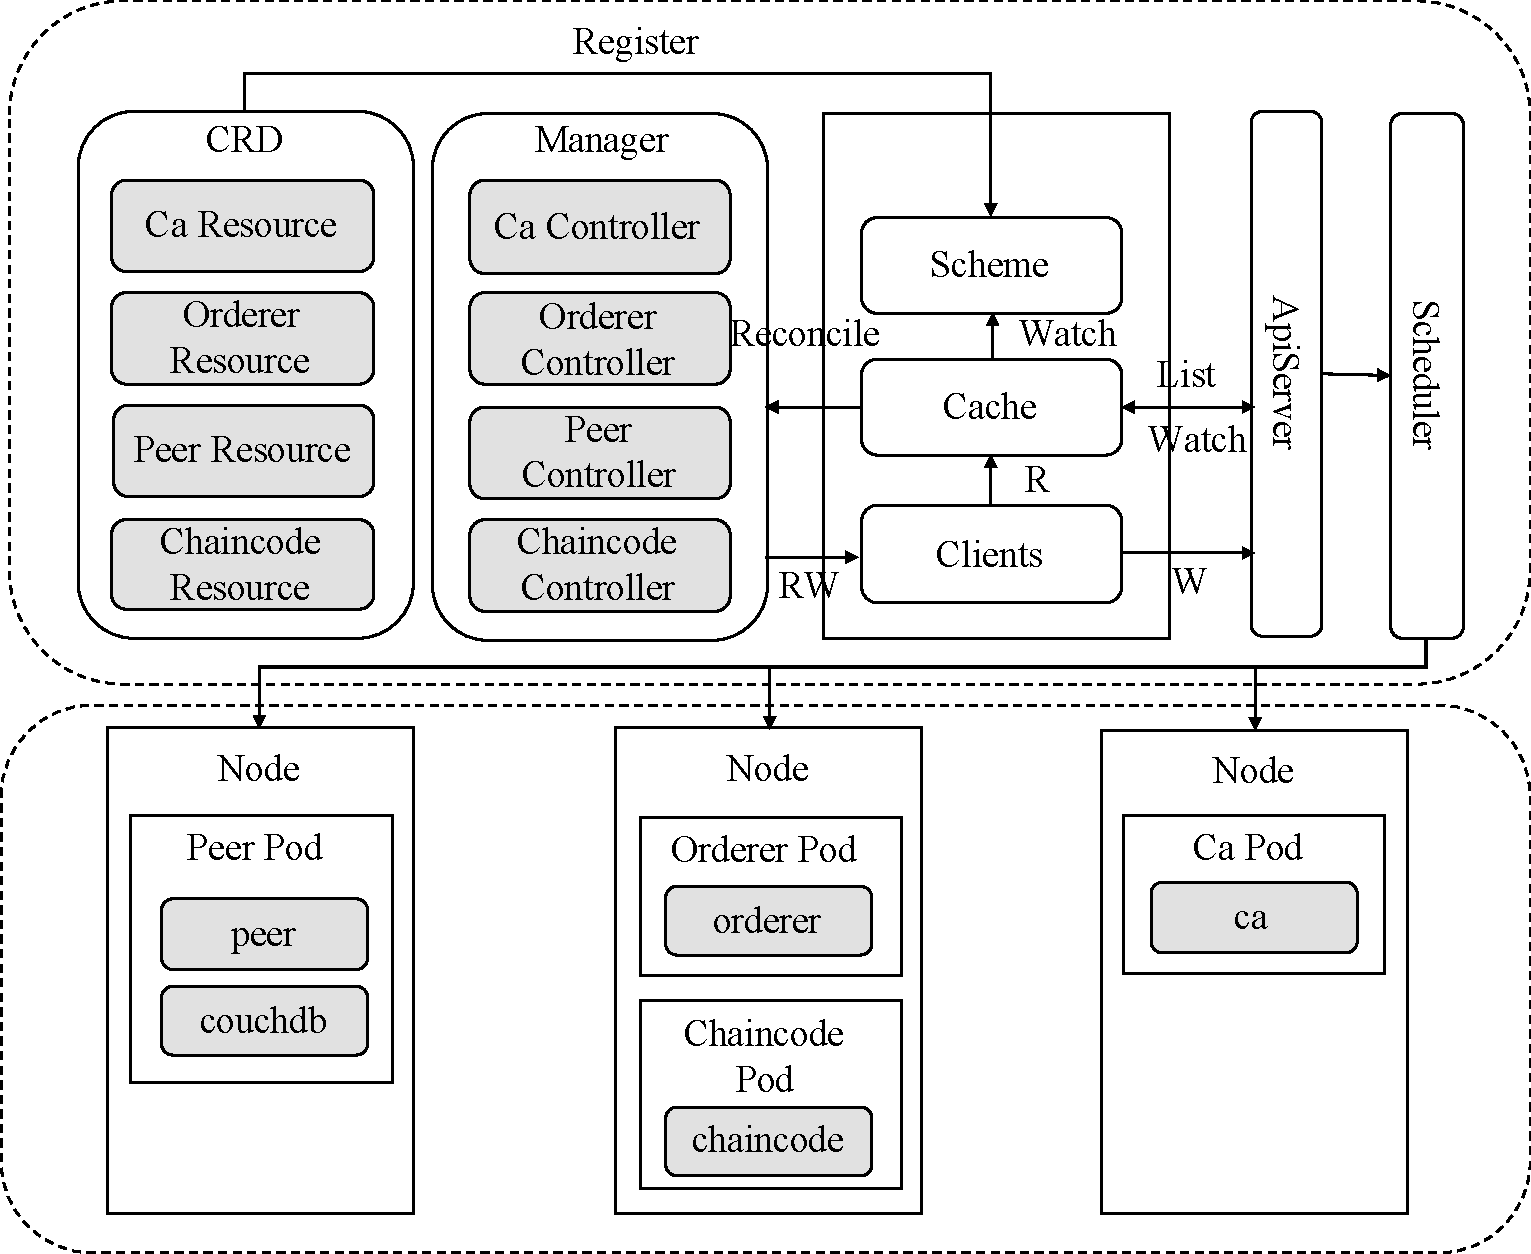
\includegraphics[width=1.0\textwidth]{FIGs/chapter5/manager.pdf} %中括号中的参数是设置图片充满文档的大小,你也可以使用小数来缩小图片的尺寸。
    \caption{Manager监听CR} %caption是用来给图片加上图题的
    \label{manager} %这是添加标签,方便在文章中引用图片。
\end{figure}%figure环境

在Manager内部管理了多个CR, 就需要使用多个Controller进行协调循环。这有助于关注点分离和代码的可读性。图\ref{manager}展示的是Manager监听CR的全过程。首先, 需要在CR中指定HF网络各节点所期望的状态, CRD会提前注册进入Scheme, 其提供了APIServer中GVK(Group Version Kind)与CR资源类型的映射, 通过资源类型Controller就能获取CR所定义的期望状态; 其次, Cache通过List-Watch机制与APIServer进行通信用以同步监听HF网络各节点在Kubernetes集群中的创建、删除、更新等操作, Cache可以获取HF网络各节点的实际状态; 最后, Controller循环监听期望状态与实际状态, 若期望状态与实际状态不一致, 则通过调用Clients更新、缩放、扩展、备份等操作进行协调一致。

区块链云化框架遵循标准化原则为HF网络中的各节点提供了标准化的Helm chart模板。在Helm中复用HF网络节点镜像(S1)并利用Kubernetes进行编排和管理底层的物理资源。这可以使用户能够轻松地在集群之间移动和部署云化框架及HF网络, 确保区块链系统基础架构的云独立性, 取消对云提供商的强依赖性, 提升本框架的可移植性与通用性。


\begin{figure}[h] %figure环境,h默认参数是可以浮动,不是固定在当前位置。如果要不浮动,你就可以使用大写float宏包的H参数,固定图片在当前位置,禁止浮动。
    \centering %使图片居中显示
    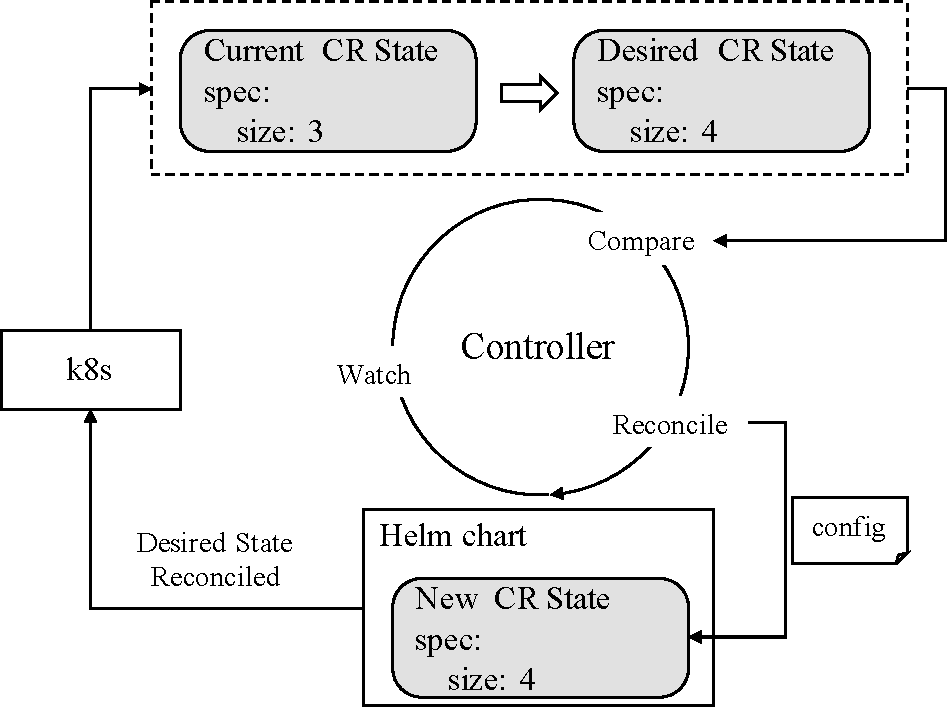
\includegraphics[width=0.75\textwidth]{FIGs/chapter5/controller.pdf} %中括号中的参数是设置图片充满文档的大小,你也可以使用小数来缩小图片的尺寸。
    \caption{Controller循环监听} %caption是用来给图片加上图题的
    \label{controller} %这是添加标签,方便在文章中引用图片。
\end{figure}%figure环境

为提升区块链云化框架的生产效率, 本文设计了一套针对HF Helm的Controller(S3), 直接将提前配置好的Helm随CRD以及Controller一起部署进Kubernetes。Helm通过调用Kubernetes的APIServer逐个将Helm chart中的yaml推送给Kubernetes。但Helm的弊端是缺乏对资源的全生命期监控, 只有CRD才能持续监听Kubernetes资源对象的变化事件, 进行全生命期监控响应。一旦创建新的CR, Controller根据对应的资源对象更新Helm的模板参数并重新部署入Kubernetes集群。图\ref{controller}以spec.size为例展示了Controller更新Helm的流程。本框架不仅通过Helm简化部署流程, 并且还能实现带全生命周期管理的Helm效果。根据这个特性, 每个CR中对应的属性一旦经过管理员更改即可反馈到Kubernetes以及HF网络中, 这能够在不介入网络的情况下的修改、配置HF网络。


% 存储扩展性
除第\ref{section: Custom_Resource_Definition}节所提到的利用CRD对HF网络配置进行模块化设计外, 本框架在Helm中为每个运行中的HF网络节点选择PVC(S4)作为链外存储, 并为每个PVC中预留出一定的额外存储资源。这相较于对所有持久存储的服务使用一个PVC而言, 虽然增加额外的存储资源冗余, 但拥有更多的PVC能够保障每个网络节点拥有足够的存储空间, 以便在不缺乏存储资源的情况下正确运行节点。拥有更多的PVC增加了首次部署难度及过度调配的风险, 但多PVC能够灵活针对不同节点运行情况利用Kubernetes进行有针对性的存储扩容, 增强框架对于存储的扩展性。尽管多PVC在管理方面存在一定的复杂性, 但在选择多PVC更加符合最佳实践, 并且效率更高\cite{d2020design}。具体地, 框架首先部署基础StorageClass并针对于HF网络中的所有Ca、Orderer、Peer节点都会设置专属PVC存储单元。这些存储单元会根据CRD的定义挂载到具体的网络节点, 网络节点生成的交易数据将会高效的写入可插拔式的持续久化介质里面。

如图\ref{pvc_sc}所示, 当创建Peer节点并输入需要多少容量的CouchDB时, 框架会为管理员定制生成对应的Peer CR, 并按照前面所述流程更新Helm。此时, Kubernetes会根据PVC进行适配寻找合适的PV进行存储。PVC只是针对于存储的声明并不会进行真正的存储, 其服务于Peer Pod。框架在定义StorageClass时会将“allowVolumeExpansion”字段设置为“true”, 这会允许PVC的扩容操作。 当初始设定的初始存储值不够时, 可以通过修改CR中的PVC的容量进行动态的灵活扩容。链外存储使得账本数据与操作独立实现, “账本数据生于链却独立于链”, 能够更好地支持数据治理。

\begin{figure}[h] %figure环境,h默认参数是可以浮动,不是固定在当前位置。如果要不浮动,你就可以使用大写float宏包的H参数,固定图片在当前位置,禁止浮动。
    \centering %使图片居中显示
    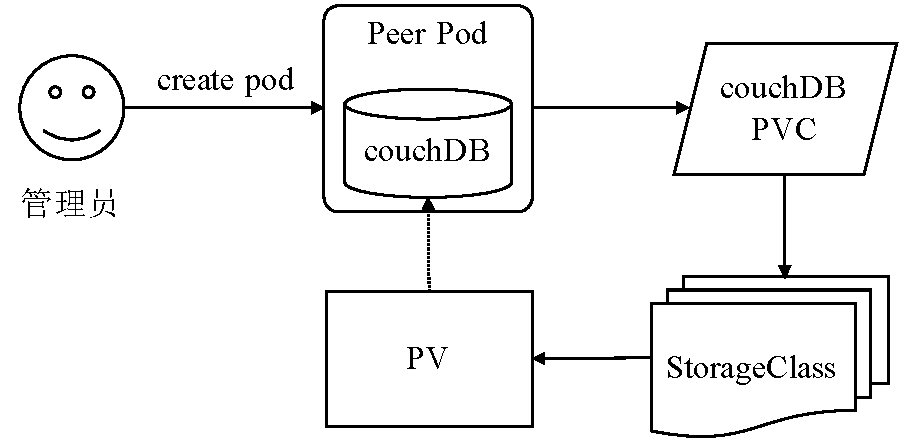
\includegraphics[width=0.75\textwidth]{FIGs/chapter5/pvc_sc.pdf} %中括号中的参数是设置图片充满文档的大小,你也可以使用小数来缩小图片的尺寸。
    \caption{原型工具存储策略} %caption是用来给图片加上图题的
    \label{pvc_sc} %这是添加标签,方便在文章中引用图片。
\end{figure}%figure环境

% 安全性
在安全性方面区块链云化框架复用Kubernetes的原生安全保障体系, 主要涉及到两方面。 一方面是Kubernetes集群中用户对框架操作的访问控制限制。区块链云化框架会生成很多清单文件向Kubernetes集群中部署HF网络, 此时框架将所有资源放入同一命名空间下(S7)。由于Kubernetes没有以用户身份进行身份验证, 所以框架采用RBAC(S5)将对同一命名空间下资源操作的最小权限映射到框架中的Manager及HF网络节点。对于自定义生成的资源, 设置了两种类型的角色(ClusterRole)分别是editor以及viewer, 如图\ref{safety}-I展示了viewer角色的权限, editor相较于viewer则增加了create、delete、update、patch的权限, 使用ClusterRoleBinding将角色与用户(ServiceAccount)进行捆绑。值得注意的是, 区块链云化框架无需以root身份运行, 在确保HF网络正常工作的同时, 应尽可能限制访问。上述安全策略只是保护HF网络的第一道防线, 另一方面是防止非法用户参与HF网络内部交易流程以及数据篡改。在经过Ca节点生成用户密码后, 框架避免使用直接向节点镜像中注入环境变量的方式管理密码信息。如图\ref{safety}-II所示, 本框架采用Secret(S6)配合x509\cite{8249485}存储管理导出的敏感密钥数据, 这种方式不但能提高灵活性而且增加了密码的传输、存储、访问安全, 增强隐私保护。

\begin{figure}[h] %figure环境,h默认参数是可以浮动,不是固定在当前位置。如果要不浮动,你就可以使用大写float宏包的H参数,固定图片在当前位置,禁止浮动。
    \centering %使图片居中显示
    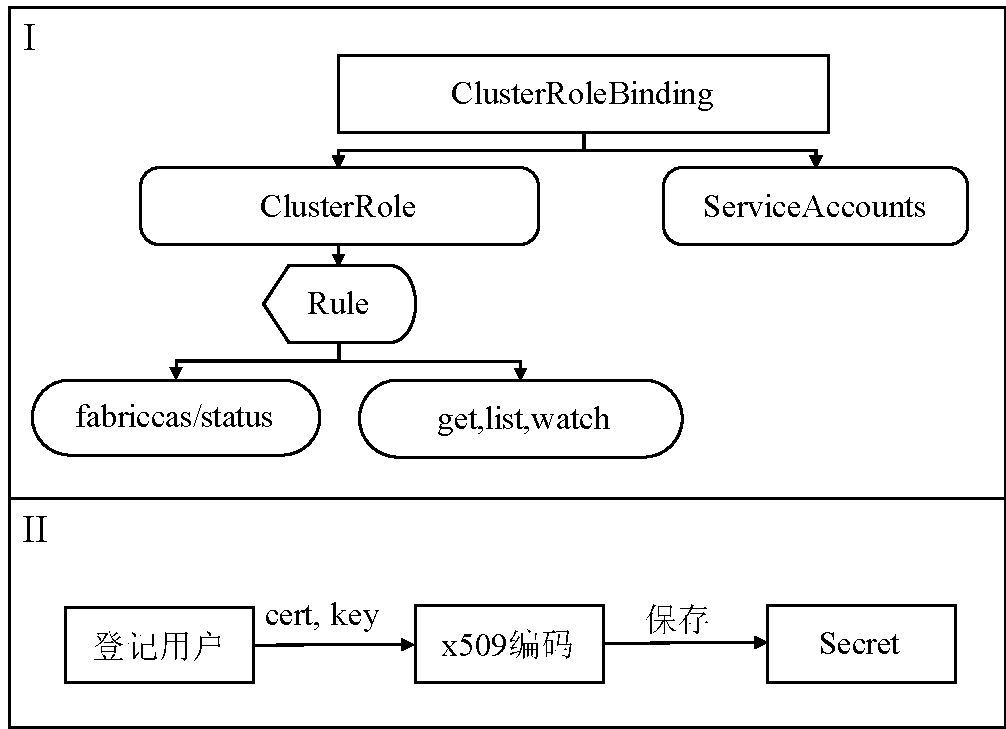
\includegraphics[width=0.75\textwidth]{FIGs/chapter5/safety.pdf} %中括号中的参数是设置图片充满文档的大小,你也可以使用小数来缩小图片的尺寸。
    \caption{原型工具安全策略} %caption是用来给图片加上图题的
    \label{safety} %这是添加标签,方便在文章中引用图片。
\end{figure}%figure环境

% 可靠性
本框架采用非介入式的云上监控方案Prometheus以及Grafana进行可视运维(S9), 在CRD中预留Exporter、ServiceMonitor等属性, 对应的在Helm chart中定制抓取周期等相关配置对HF网络中的Ca、Orderer、Peer、CouchDB、链码等进行可视化监控。同时, Grafana开源特性能够创建自定义插件, 以及图形化的方式运维区块链网络。通过Prometheus监控体系能够实时监控区块链网络的运行状态, 帮助HF网络管理人员及时发现并解决问题, 提升本框架的可靠性。

HF 2.0之前链码打包安装于Peer节点内部, 这是一种强耦合的关系。HF 2.0之后引入了外部链码的新生命周期, 即可以支持链码在Peer节点外部构建与启动。如图\ref{external_cc}展示了智能合约部署原理。值得注意的是, 该流程仅展示流水线的核心部署环节。本框架为链码定制Dockerfile模板以及Kubernetes部署文件, 使单个链码进行容器化部署托管于集群之上。然后, 将该过程封装配置作为持续交付流水线中核心的智能合约部署环境。同时, 每次智能合约进行升级时, 只需修改合约代码即可完成自动升级。通过智能合约微服务化流程可以极大的提高链码部署、升级过程的灵活性。本框相较于Mictract在部署中的做了如下优化: (1)取消NFS外部文件服务器的方式, 利用Secret保存密钥文件;(2) 将环境变量注入链码CRD作为输入, 而不是直接硬编码Deployment配置文件。

\begin{figure}[h] %figure环境,h默认参数是可以浮动,不是固定在当前位置。如果要不浮动,你就可以使用大写float宏包的H参数,固定图片在当前位置,禁止浮动。
    \centering %使图片居中显示
    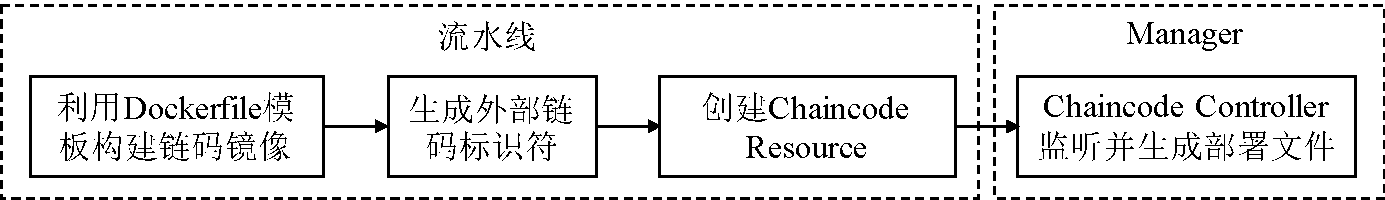
\includegraphics[width=1.0\textwidth]{FIGs/chapter5/external_cc.pdf} %中括号中的参数是设置图片充满文档的大小,你也可以使用小数来缩小图片的尺寸。
    \caption{智能合约微服务部署原理} %caption是用来给图片加上图题的
    \label{external_cc} %这是添加标签,方便在文章中引用图片。
\end{figure}%figure环境


最后, 本框架对外采用动态命令式查询(S10), 对内封装创建、更新、删除HF网络各节点以及通道、链码相关功能模块的各项操作。通过命令查询的方式, 可以大大降低区块链云化框架的使用门槛, 无需关心内部复杂的证书、网络等创建逻辑。

\subsection{Hyperledger Fabric网络}

HF网络是一个复杂的分布式系统, 需要权衡速度、性能等条件对不同网络节点的部署状态进行合理设计。静态节点Ca、Orderer、Peer在首次启动网络时就需要部署在Kubernetes集群中并以Pod形式运行。Pod是Kubernetes中可以创建和部署的最小单位。在Kubernetes集群中, Pod内的容器有两种运行状态:

\begin{itemize}[itemindent=2em]
    \item 单容器: Pod当作单容器进行封装, Kubernetes管理的是Pod而非容器;

    \item 多容器: 当容器间需要紧密协作时可以在同一Pod中运行多容器。
\end{itemize}

Ca是HF网络中的证书授权中心, Orderer负责交易的排序, 这两个节点在配置上需要满足可插拔式设计。 但在网络运行时, 需要各自在一个Pod中运行即可, 同时 在一个Pod中运行可以有效地利用Kubernetes的自动缩放功能进行弹性伸缩。

Peer是HF网络中被使用最多的模块, 是HF网络的基石, 其负责区块链数据的存储以及运行链码。由于Peer节点需要频繁地与账本存储单元如CouchDB进行交互, 所以Peer容器应当与CouchDB容器存在于同一Pod中。在同一个Pod中, Peer容器与CouchDB紧密协作, 拥有相同的存活周期, 更优的, 相同Pod中的不同容器共享进程、IP地址和数据卷, 可以进行频繁的文件和数据交换。Peer支持外部链码部署, 即链码拥有自己独立的Pod运行环境, 这能够纳入智能合约微服务化流程进行快速响应与监控。 

\section{原型工具}

\subsection{工具概述}

\begin{figure}[!htbp] %figure环境,h默认参数是可以浮动,不是固定在当前位置。如果要不浮动,你就可以使用大写float宏包的H参数,固定图片在当前位置,禁止浮动。
    \centering %使图片居中显示
    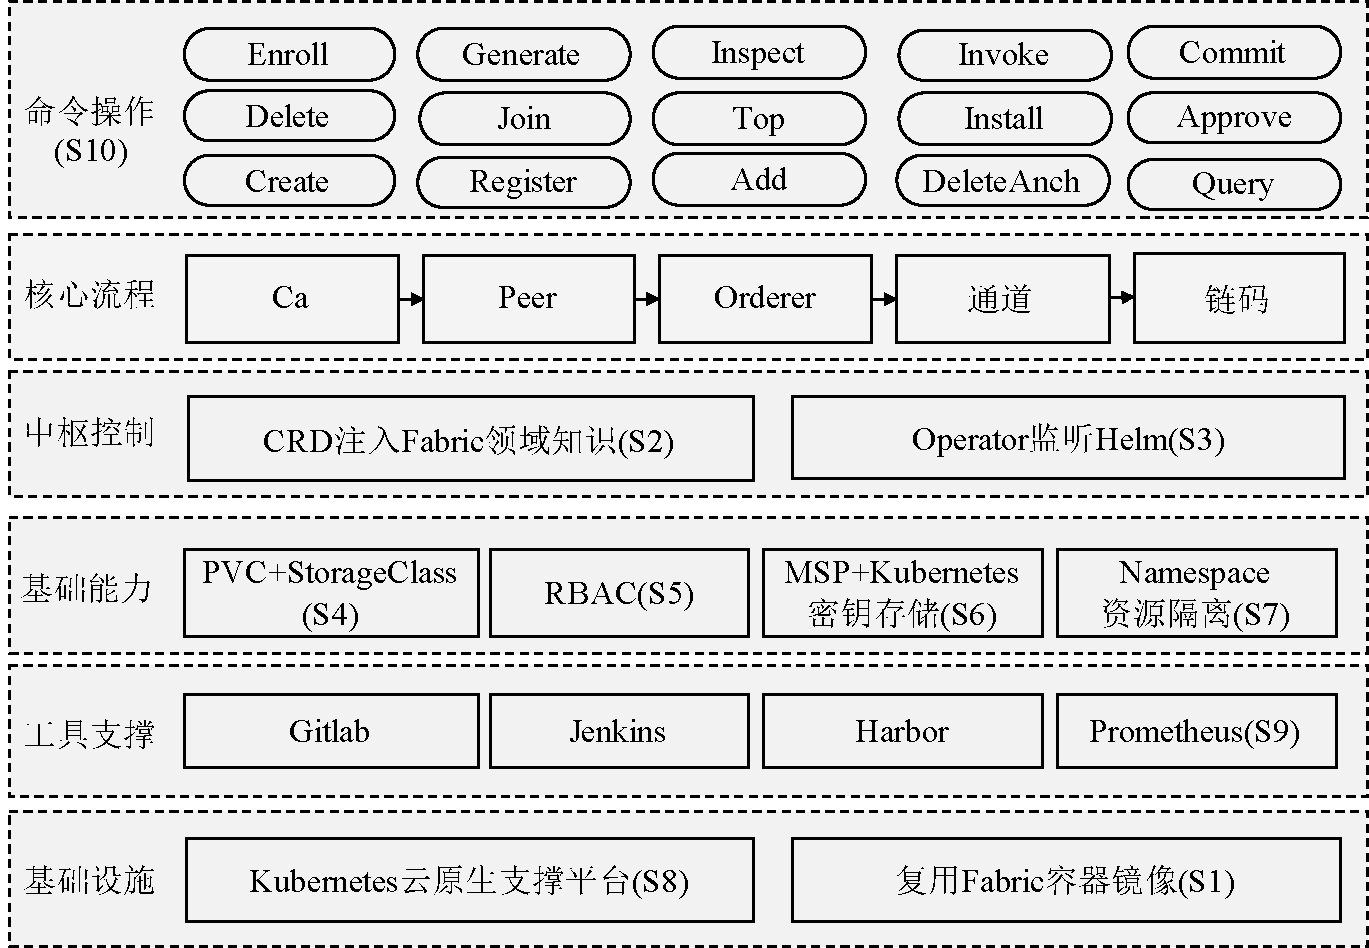
\includegraphics[width=1.0\textwidth]{FIGs/chapter5/tool.pdf} %中括号中的参数是设置图片充满文档的大小,你也可以使用小数来缩小图片的尺寸。
    \caption{原型工具总体功能} %caption是用来给图片加上图题的
    \label{toolstotal} %这是添加标签,方便在文章中引用图片。
\end{figure}%figure环境

云原生具有资源按需配置, 动态伸缩的特性。当前, BaaS虽然能够基于云平台构建区块链系统, 但仅提供脚本化的方式部署区块链网络及智能合约, 仍未深入云基础设施平台的底层有效利用云的特性管理区块链平台, 这导致了BaaS平台对云特性的严重浪费。因此, 一个支持区块链有效云化的工具十分重要。如图\ref{toolstotal}所示, 本文基于提出区块链云化框架提供配套的面向Hyperledger Fabric的区块链云化原型工具。原型工具建立在HF核心流程之上, 对外以命令的方式动态管理整个HF网络, 以持续交付的流程部署智能合约, 对内声明式配置HF网络中的Ca、Orderer、Peer实体, 利用可移植性、可靠性、易用性、可扩展性以及安全性等策略为HF网络赋能。


\subsection{需求分析} \label{section: requirement}

本节重点介绍原型工具的功能性需求, 如图\ref{fabric_use_case}所示, HF网络管理人员期望能够通过原型工具对HF网络各节点分别进行命令式启停, 降低HF网络的启动时间成本。

\begin{figure}[!htbp] %figure环境,h默认参数是可以浮动,不是固定在当前位置。如果要不浮动,你就可以使用大写float宏包的H参数,固定图片在当前位置,禁止浮动。
    \centering %使图片居中显示
    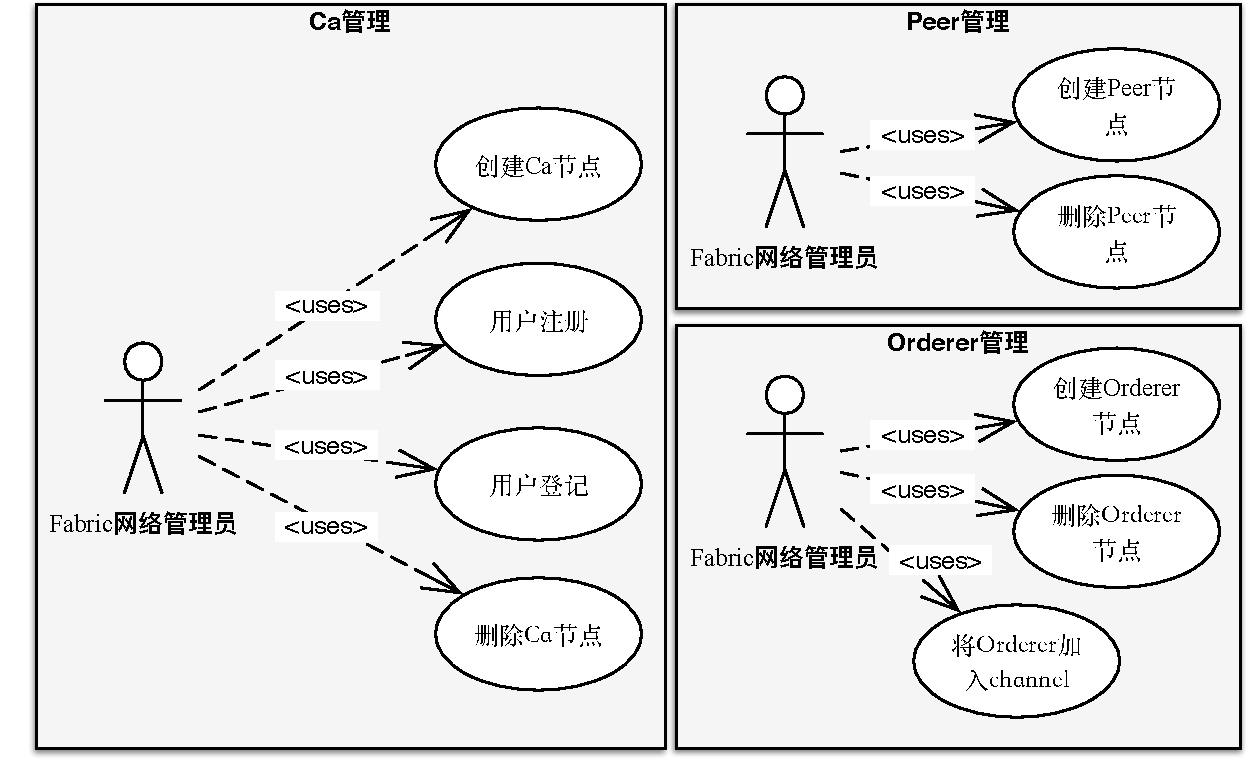
\includegraphics[width=1.0\textwidth]{FIGs/chapter5/fabric_use_case.pdf} %中括号中的参数是设置图片充满文档的大小,你也可以使用小数来缩小图片的尺寸。
    \caption{HF网络管理用例图} %caption是用来给图片加上图题的
    \label{fabric_use_case} %这是添加标签,方便在文章中引用图片。
\end{figure}%figure环境

表\ref{ca_use_case}展示了Ca管理的用例描述, Ca管理需为HF网络管理人员提供灵活方便的启停Ca节点的功能, 同时提供注册、签发证书的功能。在启动过程中应以命令行参数配置的方式设置Ca启动所可选的配置项, 如Database、Host、CLRSizeLimit等。同样, Ca管理需要覆盖Ca节点原有的用户注册、用户登记等基本功能。

{\footnotesize
\begin{longtable}[h]{m{60pt}|m{280pt}}
    \caption[Ca管理用例表]{Ca管理用例表} \label{ca_use_case} \\
        \hline  
        ID&UC-Ca\\
        \hline
        名称&可视化建模用例\\
        \hline
        描述&HF网络管理员可以通过命令的方式创建、删除Ca节点, 并能够以命令行参数的形式将Ca启动参数注入。 同时, HF网络管理员能够无障碍进行用户注册、登记。\\
        \hline
        触发条件&HF网络管理员输入对应Ca命令\\
        \hline
        前置条件&Kubernetes集群环境\\
        \hline
        后置条件&无\\
        \hline
        正常流程& (1)HF网络管理员输入“kubectl hf ca create”并以可选参数的形式输入其他如Ca名称、容量等配置项
        \newline (2)HF网络管理员输入“kubectl hf ca register”并以可选参数的形式输入其他如用户名、密码等配置项
        \newline (3)HF网络管理员输入“kubectl hf ca enroll”并输入已经注册过的用户名、密码等信息将注册的用户进行登记并导出证书信息
        \newline (4)可选的, HF网络管理员输入“kubectl hf ca delete”删除ca节点 \\
        \hline
        异常流程&无\\
        \hline
    \end{longtable} 
}

表\ref{peer_use_case}展示了Peer管理的用例描述, Peer管理需为HF网络管理人员提供灵活方便的启停Peer节点的功能, 在启动过程中应以内置命令行参数配置的方式设置Peer启动所可选的配置项, 如Peer对应的Ca名称账本存储类型、Gossip协议、组织信息等。

{\footnotesize
\begin{longtable}[h]{m{60pt}|m{280pt}}
    \caption[Peer管理用例表]{Peer管理用例表} \label{peer_use_case} \\
        \hline  
        ID&UC-Peer\\
        \hline
        名称&可视化建模用例\\
        \hline
        描述&HF网络管理员可以通过命令方式创建、删除Peer节点, 并能够以命令行参数的形式将Peer启动参数注入。\\
        \hline
        触发条件&HF网络管理员输入对应Peer命令\\
        \hline
        前置条件&已经启动对应组织级的Ca\\
        \hline
        后置条件&无\\
        \hline
        正常流程& (1)HF网络管理员输入“kubectl hf peer create”并以可选参数的形式输入其他如Peer名称、所属组织、账本存储类型等配置项
        \newline (2)可选的, HF网络管理员输入“kubectl hf peer delete”删除Peer节点 \\
        \hline
        异常流程& HF网络管理员输入的对应Ca名称匹配不上, 报错提示\\
        \hline
    \end{longtable} 
}

表\ref{orderer_use_case}展示了Orderer管理的用例描述, Orderer管理需为HF网络管理人员提供灵活方便的启停Orderer节点的功能, 同时能够将Orderer加入到通道中,在启动过程中应以内置命令行参数配置的方式设置Orderer启动所可选的配置项, 如Orderer对应的Ca名称、自己的名称、组织、容量等信息。



{\footnotesize
\begin{longtable}[h]{m{60pt}|m{280pt}}
    \caption[Orderer管理用例表]{Orderer管理用例表} \label{orderer_use_case} \\
        \hline  
        ID&UC-Orderer\\
        \hline
        名称&可视化建模用例\\
        \hline
        描述&HF网络管理员可以通过命令的方式创建、删除Orderer节点, 并能够以命令行参数的形式将Orderer启动参数注入。\\
        \hline
        触发条件&HF网络管理员输入对应Orderer命令\\
        \hline
        前置条件& (1)已经启动对应组织级的Ca
        \newline (2)Orderer加入通道前确保通道建立\\
        \hline
        后置条件&无\\
        \hline
        正常流程& (1)HF网络管理员输入“kubectl hf orderer create”并以可选参数的形式输入其他如Orderer名称、所属组织、所属组织的Ca名称等配置项
        \newline (2)HF网络管理员输入“kubectl hf orderer join” 并以参数的形式输入名称、命名空间、输入创世区块信息、自己的证书文件
        \newline (3)HF网络管理员输入“kubectl hf orderer delete”以删除Orderer \\
        \hline 
        异常流程& Orderer节点证书文件验证不通过, 禁止加入\\
        \hline
    \end{longtable} 
}

\begin{figure}[!htbp] %figure环境,h默认参数是可以浮动,不是固定在当前位置。如果要不浮动,你就可以使用大写float宏包的H参数,固定图片在当前位置,禁止浮动。
    \centering %使图片居中显示
    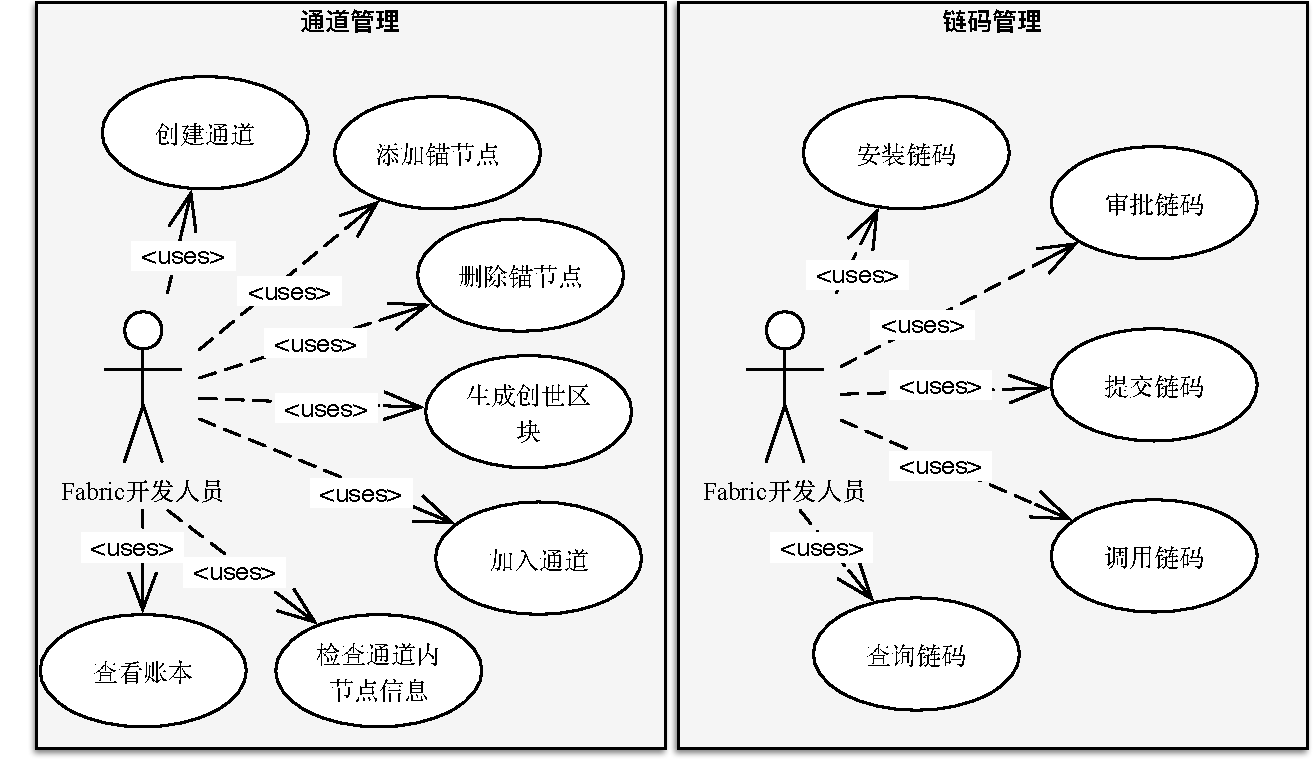
\includegraphics[width=1.0\textwidth]{FIGs/chapter5/chan_cc_use_case.pdf} %中括号中的参数是设置图片充满文档的大小,你也可以使用小数来缩小图片的尺寸。
    \caption{通道管理用例图} %caption是用来给图片加上图题的
    \label{chan_cc_use_case_pic} %这是添加标签,方便在文章中引用图片。
\end{figure}%figure环境

除管理HF网络节点外, 如图\ref{chan_cc_use_case_pic}所示, 本文展示了通道管理以及链码管理的用例图, HF开发人员期望能够通过原型工具完成管理通道和操作链码的各项操作。表\ref{chan_use_case}展示了通道管理的用例描述, 通道管理需为HF开发人员屏蔽大量证书文件提供灵活方便地开启通道的功能, 应以内置命令行参数配置的方式配置通道, 包含对通道内部锚节点、创世区块、账本的管理。表\ref{cc_use_case}展示了链码管理的用例描述, 链码管理需为HF网络开发人员提供灵活方便的安装、提交链码等功能。


{\footnotesize
\begin{longtable}[h]{m{60pt}|m{280pt}}
    \caption[通道管理用例表]{通道管理用例表} \label{chan_use_case} \\
        \hline  
        ID&UC-Chan\\
        \hline
        名称&可视化建模用例\\
        \hline
        描述&HF开发人员可以通过命令的方式创建、管理通道\\
        \hline
        触发条件&HF开发人员输入对应通道命令\\
        \hline
        前置条件&已经启动好基础HF网络, 包含Ca、Orderer、Peer\\
        \hline
        后置条件&无\\
        \hline
        正常流程& (1)HF开发人员输入“kubectl hf channel generate”并以可选参数的形式输入所包含的组织名称以及输出的创世区块保存文件
        \newline (2)HF开发人员输入“kubectl hf channel join” 并以参数的形式输入应当加入该通道的节点名称、组织信息和用户
        \newline (3)HF开发人员员输入“kubectl hf channel addanchorpeer”并以参数的形式输入通道的名称用以向通道中加入锚节点
        \newline (4)HF开发人员员输入“kubectl hf channel top”并以参数的形式输入通道的名称用以向查询账本的高度 \\
        \hline 
        异常流程& 无 \\
        \hline
    \end{longtable} 
}


{\footnotesize
\begin{longtable}[h]{m{60pt}|m{280pt}}
    \caption[链码管理用例表]{链码管理用例表} \label{cc_use_case} \\
        \hline  
        ID&UC-CC\\
        \hline
        名称&可视化建模用例\\
        \hline
        描述&HF开发人员可以通过命令的方式安装、提交、查询链码;\\
        \hline
        触发条件&HF开发人员输入对应链码命令\\
        \hline
        前置条件&已经部署好通道\\
        \hline
        后置条件&无\\
        \hline
        正常流程& (1)HF开发人员输入“kubectl hf chaincode intall”并以可选参数的形式输入链码地址、链码语言、标签等参数用以安装链码
        \newline (2)HF开发人员输入“kubectl hf chaincode approveformyorg" 并以参数的形式传入链码package-id、链码名称、组织信息、策略等参数用以所在组织审批链码
        \newline (3)HF开发人员输入“kubectl hf chaincode commit”并以参数的形式输入链码名称、策略等信息用以提交链码
        \newline (4)HF开发人员输入“kubectl hf chaincode invoke”并以参数的形式输入链码名称、调用方法等信息用以调用链码
        \newline (5)HF开发人员输入“kubectl hf chaincode query”并以参数的形式输入链码名称、调用方法等信息用以查询链码\\
        \hline 
        异常流程& (1)因网络原因安装链码时间过长而导致, 提示并报错。\\
        \hline
    \end{longtable} 
}

\subsection{设计与实现}

面向Hyperledger Fabric的区块链云化工具是一个基于Kubernetes Operator的应用, 其整合Helm用以完成HF网络的快速部署和节点的全生命周期管理。 为完成命令式查询原型工具采用Cobra\footnotemark[1]\footnotetext[1]{\href{https://github.com/spf13/cobra}{cobra github地址}}完成命令的封装。由于原型工具在管理Ca、Orderer、Peer各节点时, 处理逻辑存在重复性, 故本节将以Ca节点作为案例介绍详细介绍网络节点针对需求分析的设计与实现。

% create CRD
当HF网络管理员需要创建Ca并输入对应的命令及参数时, 如图\ref{create_crd}所示, 原型工具首先解析输入参数的合法性, 然后将对应的输入参数填充到已经定义好的FabricCA模版中,最后调用Kubernetes Client将Fabric Ca Resource依据CRD的规则部署进入集群中。伪代码\ref{code1}展示了创建Ca Resource的伪代码。

\begin{figure}[!htbp] %figure环境,h默认参数是可以浮动,不是固定在当前位置。如果要不浮动,你就可以使用大写float宏包的H参数,固定图片在当前位置,禁止浮动。
    \centering %使图片居中显示
    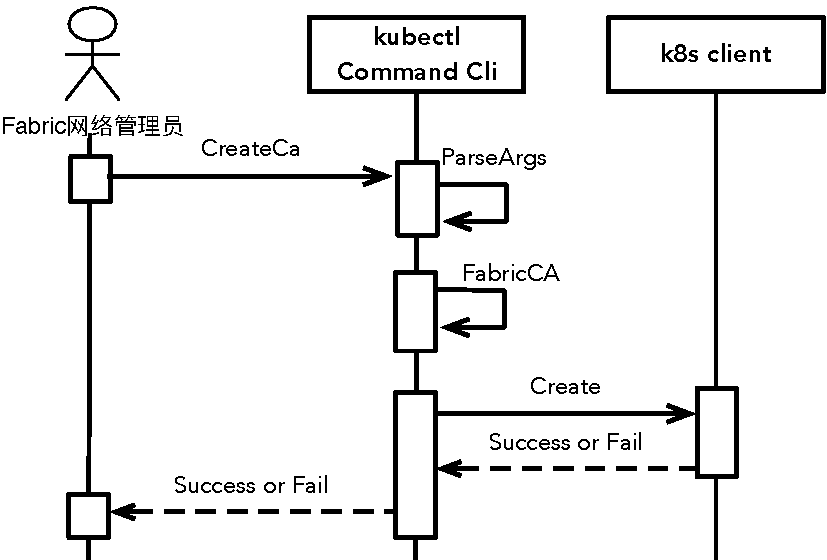
\includegraphics[width=0.75\textwidth]{FIGs/chapter5/create_crd.pdf} %中括号中的参数是设置图片充满文档的大小,你也可以使用小数来缩小图片的尺寸。
    \caption{创建Ca Resource时序图} %caption是用来给图片加上图题的
    \label{create_crd} %这是添加标签,方便在文章中引用图片。
\end{figure}%figure环境


\begin{algorithm}[!htbp]
    \floatname{algorithm}{\footnotesize 伪代码}
    \caption{\footnotesize 创建Ca Resource伪代码}
    \label{code1}
    {\footnotesize
    \begin{algorithmic}
        \renewcommand{\algorithmicrequire}{ \textbf{Input:}}
        \REQUIRE  
        “kubectl ca create” with args

        \renewcommand{\algorithmicensure}{\textbf{Output:}}
        \ENSURE
        Success or Fail

        \STATE{err := ParseArgs()}

        \STATE{client, err := GetKubeOperatorClient()}

        \STATE{fabricCa := \&v1alpha1.FabricCA\{Initialization according to parameters\}}

        \IF{args.output}
            \STATE{out, err := yaml.Marshal(\&fabricCa)} 
        \ELSE
            \STATE{err := client.FabricCA(namespaces).Create(fabricCa)}
        \ENDIF

        \STATE{return success}
    \end{algorithmic}
    }
\end{algorithm}

当Fabric Ca Resource一旦被部署到集群中就会被处理单元Manager中的Ca  Controller探查到其存活。如图\ref{reconcile}所示, Ca Controller通过Reconcile循环探听Ca Resource。由于资源被删除后再也无法获取到被删除资源的信息, 所以利用Finalizer字段进行标识, GetDeletetionTimeStamp()用于获取CR被删除时的时间戳。一旦探听到Ca Resource的存在就会先处理Finalizer字段。DeletionTimestamp不为空时, Controller会轮询该CR的更新请求执行处理所有的Finalizer。随后, Ca Controller会检查当前是否存在Ca Helm release, 若不存在则将当前状态Ca Resource所定义的TLS、CFG等信息生成Helm chart并将其部署进入集群中; 若存在则先获取当前Ca Resource的状态并对其进行更新之后再生成Helm chart部署。Helm chart中定义了Ca启动所需要的全部如Deployment、Service、Istio、ServiceMonitor等Yaml, 通过启动Helm就可以一次性将其全部启动部署。伪代码\ref{code2}展示了Ca Controller Reconcile的相关代码。

\begin{figure}[!htbp] %figure环境,h默认参数是可以浮动,不是固定在当前位置。如果要不浮动,你就可以使用大写float宏包的H参数,固定图片在当前位置,禁止浮动。
    \centering %使图片居中显示
    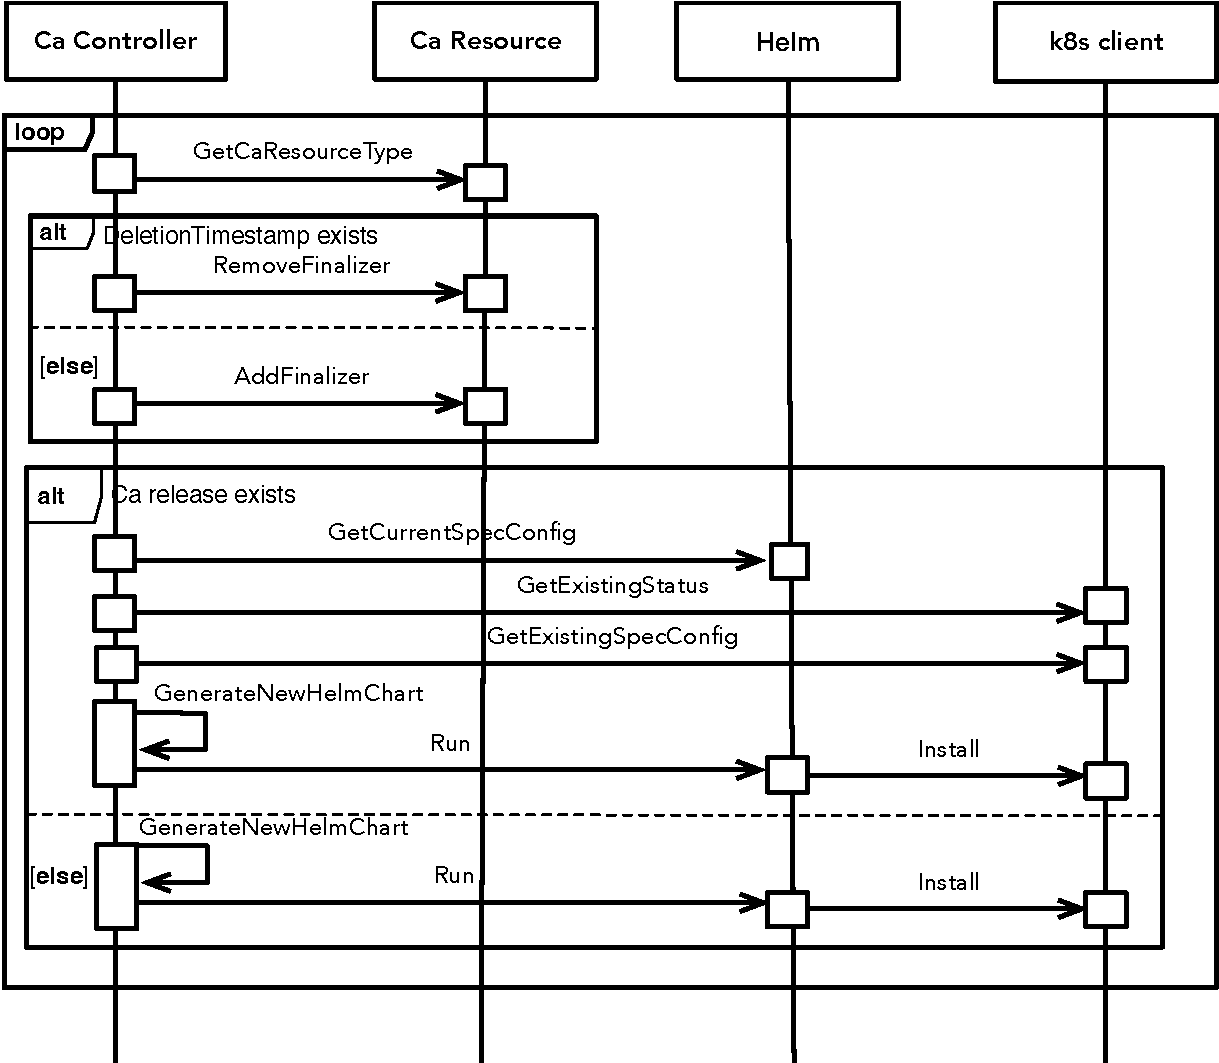
\includegraphics[width=1.0\textwidth]{FIGs/chapter5/reconcile.pdf} %中括号中的参数是设置图片充满文档的大小,你也可以使用小数来缩小图片的尺寸。
    \caption{Ca Controller Reconcile逻辑时序图} %caption是用来给图片加上图题的
    \label{reconcile} %这是添加标签,方便在文章中引用图片。
\end{figure}%figure环境

\begin{algorithm}[!htbp]
    \floatname{algorithm}{\footnotesize 伪代码}
    \caption{\footnotesize Ca Controller Reconcile伪代码}
    \label{code2}
    {\footnotesize
    \begin{algorithmic}
        \renewcommand{\algorithmicrequire}{ \textbf{Input:}}
        \REQUIRE  
        nil

        \renewcommand{\algorithmicensure}{\textbf{Output:}}
        \ENSURE
        nil

        \IF{fabricCa.GetDeletetionTimestamp() != nil}
            \IF{fabricCa.GetFinalizers().contains(caFinalizer)}
                \STATE{RemoveFinalizer(fabricCa, caFinalizer)} 
            \ENDIF
        \ENDIF

        \IF{!fabricCa.GetFinalizers().contains(caFinalizer)}
            \STATE{AddFinalizer(fabricCa, caFinalizer)} 
        \ENDIF

        \STATE{exits := status.Run(caReleaseName)}

        \IF{exits}
            \STATE{c := GetCurrentSpecConfig(caReleaseName)}
            \STATE{s := GetExistingStatus(caReleaseName)}
            \STATE{newCa := fabricCa.DeepCopy()}
            \STATE{newCa.Status = s.Status}

            \STATE{release := cmd.Run(caReleaseName, c)}
            \IF{!reflect.DeepEqual(newCa.Status, release.Status)}
                \STATE{err := status().Update(newCa)}
            \ENDIF 
            
        \ELSE
            \STATE{c, err := GetCurrentSpecConfig(caReleaseName)}
        
            \STATE{release := cmd.Run(caReleaseName, c)}
        \ENDIF
      
    \end{algorithmic}
    }
\end{algorithm}


\begin{figure}[!htbp] %figure环境,h默认参数是可以浮动,不是固定在当前位置。如果要不浮动,你就可以使用大写float宏包的H参数,固定图片在当前位置,禁止浮动。
    \centering %使图片居中显示
    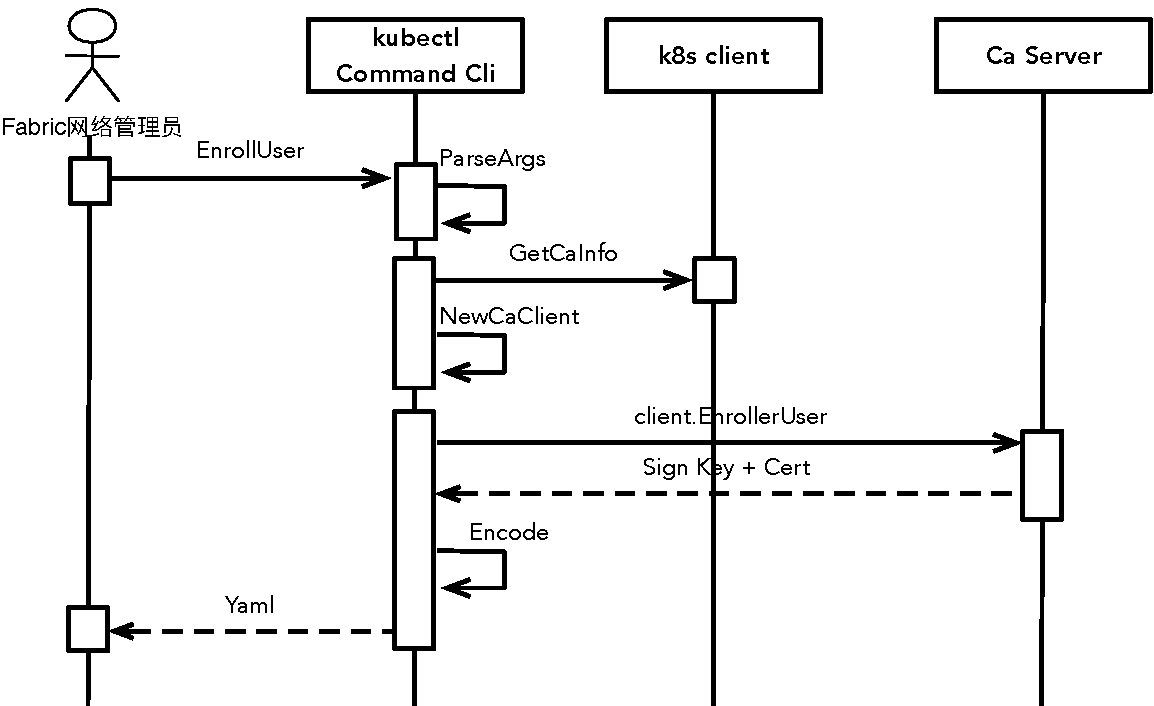
\includegraphics[width=0.9\textwidth]{FIGs/chapter5/enroll.pdf} %中括号中的参数是设置图片充满文档的大小,你也可以使用小数来缩小图片的尺寸。
    \caption{Ca Enroll User逻辑时序图} %caption是用来给图片加上图题的
    \label{enroll} %这是添加标签,方便在文章中引用图片。
\end{figure}%figure环境

成功在Kubernetes中启动后, HF网络管理员可以通过命令形式完成用户注册、用户登记的功能。如图\ref{enroll}所示, HF网络管理员输入Enroll命令以及相关参数, 原型工具会对其进行参数解析。当解析成功后, 原型工具会获取集群中Ca对外接口的相关信息, 包含URL、端口等。随后, 原型工具会生成Ca Client, 并将管理员输入的用户信息通过接口传递给Ca Server。Ca Server就是Fabric Ca在集群中的服务状态所以其具备完整的Ca的功能, 当Enroll完成后会返回key以及cert, 原型工具会利用x509对其编码并保存到yaml中返回给管理员。伪代码\ref{code3}展示了Ca Enroll User的相关代码。


\begin{algorithm}[!htbp]
    \floatname{algorithm}{\footnotesize 伪代码}
    \caption{\footnotesize Ca Enroll User伪代码}
    \label{code3}
    {\footnotesize
    \begin{algorithmic}
        \renewcommand{\algorithmicrequire}{ \textbf{Input:}}
        \REQUIRE  
        “kubectl ca enroll” with args

        \renewcommand{\algorithmicensure}{\textbf{Output:}}
        \ENSURE
        User key\&cert yaml

        \STATE{ParseArgs()}
        \STATE{client := GetKubeOperatorClient()}

        \STATE{url := GetURLForCa()}

        \STATE{crt, pk := client.EnrollUser(args.Name, args.Secret, url)}
 
        \STATE{crtPem := EncodeX509Certificate(crt)}
        \STATE{pkPem := EncodePrivateKey(pk)}

        \STATE{userYaml := yaml.Marshal(\{}
        \STATE{\quad "key": pkPem,} 
        \STATE{\quad "cert": crtPem} 
        \STATE{\})}

        \STATE{io.writeFile(args.output, userYaml)}

        \STATE{return nil}
    \end{algorithmic}
    }
\end{algorithm}


\begin{figure}[!htbp] %figure环境,h默认参数是可以浮动,不是固定在当前位置。如果要不浮动,你就可以使用大写float宏包的H参数,固定图片在当前位置,禁止浮动。
    \centering %使图片居中显示
    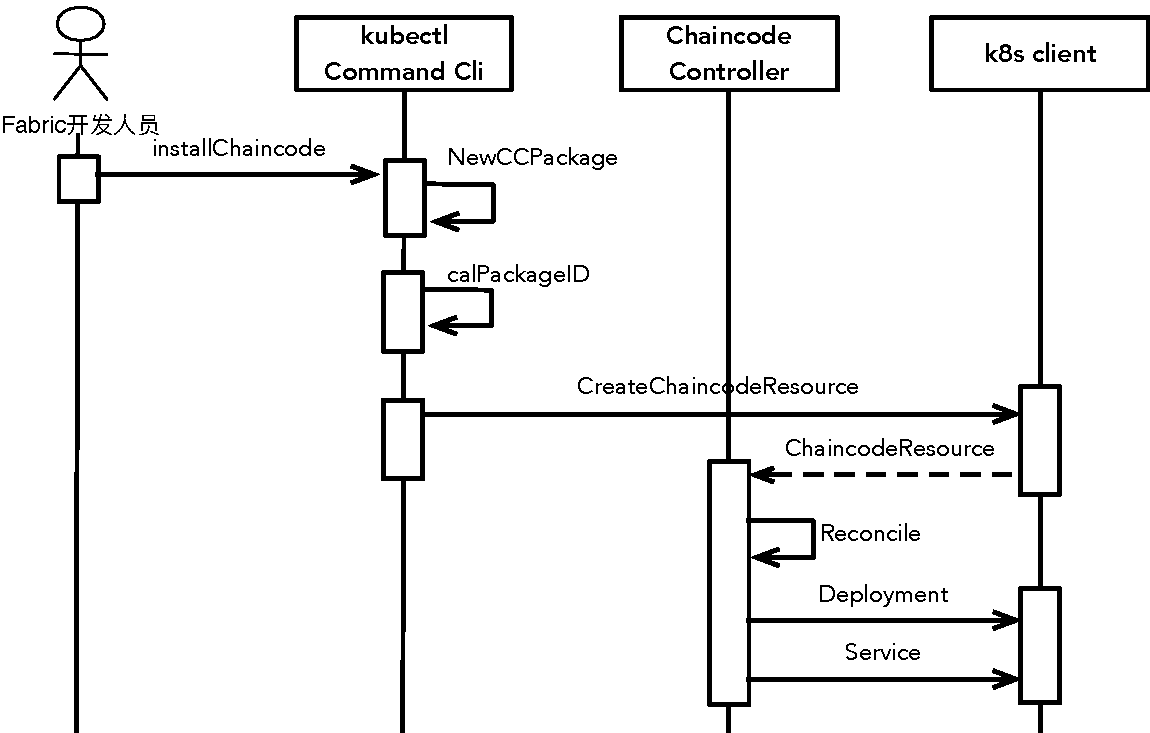
\includegraphics[width=0.9\textwidth]{FIGs/chapter5/installcc.pdf} %中括号中的参数是设置图片充满文档的大小,你也可以使用小数来缩小图片的尺寸。
    \caption{安装链码逻辑时序图} %caption是用来给图片加上图题的
    \label{installcc} %这是添加标签,方便在文章中引用图片。
\end{figure}%figure环境


当成功启动网络后, HF开发人员能够以持续交付流水线的方式或命令的方式完成链码的部署与升级。如图\ref{installcc}展示了采用命令行方式安装的过程, 安装命令可以配置进行流水线。HF开发人员输入install命令以及链码地址、用户信息等相关参数, 原型工具首先会预先根据输入的参数信息预安装链码包, 并根据预安装返回的pkgTarGzBytes生成packageID作为链码的唯一标识。然后, 原型工具会调用Kuebrnetes接口生成Chaincode Resource。一旦Chaincode Resource被部署进入集群就能够被Manager中的Chaincode Resource监听到, 并根据Chaincode Resource中所带的packageID、链码地址、数据卷信息等创建链码的Deployement以及Service。

\section{本章小节}

本章介绍了面向Hyperledger Fabric的区块链云化框架及其原型工具。首先, 给出了云化框架的工作流程、输入单元CRD、处理单元Manager以及输出单元HF网络节点运行状态。然后结合云化框架介绍了其原型工具的需求分析、设计与实现。


% \begin{itemize}[itemindent=2em]
%     \item 易用性: HF网络管理人员和开发人员在学习了基本的HF概念之后且HF网络组件镜像完备的情况下, 可以通过原型工具简化HF网络配置流程并应当在10分钟之内完成HF网络的构建;

%     \item 可靠性: 在命令输入过程中, 原型工具应当提前自动校验命令行参数的准确性, 能够判断各种异常输入并快速做出提示响应, 防止出现异常; 原型工具应当支持7*24h监控以便在工具异常时提供快速的定位手段。

%     \item 可迁移性: 原型工具需要具备便捷的安装方式, 以便于能够在支持Kubernetes的云上自由迁移;

%     \item 可扩展性: 原型工具需要为HF网络提供可插拔的标准化接口, 如共识算法、账本存储单元等; 同时, 随着交易数量的增加, 链外存储压力上升, 工具应能对存储进行动态的不重启扩容;

%     \item 安全性: 原型工具需要具备严格的权限访问控制策略, HF网络管理员(开发人员)需要经过认证之后才能有权限操作HF网络各节点的启停; 只有经过认证的HF网络用户才能进行合法交易;
% \end{itemize}




% \begin{algorithm}[!htbp]
%     \floatname{algorithm}{\footnotesize 算法}
%     \caption{\footnotesize 模型校验算法}
%     \label{algorithm1}
%     {\footnotesize
%     \begin{algorithmic}
%         \renewcommand{\algorithmicrequire}{ \textbf{Input:}}
%         \REQUIRE  
%         mxCells:HTMLCollectionOf<Element>

%         \REQUIRE
%         patterns:PatternData

%         \renewcommand{\algorithmicensure}{\textbf{Output:}}
%         \ENSURE
%         models:Map<String, Pattern>

%         \STATE{Boolean success = true;}
%         \FOR{mxCell in mxCells}

%         \STATE{patterns.setSourceToTarget(mxCell.getId, mxCell.getTarget);}

%         \STATE{patterns.setTargetToSource(mxCell.getSource, mxCell.getId);}
        
%         \ENDFOR

%         \FOR{mxCell in mxCells}
%             \IF{patterns.isParentCell(mxCell)}
%                 \IF{patterns.validation(mxCell)}
%                     \STATE{newPattern = new Pattern(mxCell);}
%                     \STATE{patterns.models.add(mxCell.getId, newPattern);}
%                 \ELSE
%                     \STATE{success = false;}
%                     \STATE{break;}
%                 \ENDIF
%             \STATE{skip loopStep;}
%             \ELSE
%             \STATE{continue loop;}
%             \ENDIF
%         \ENDFOR
          
%         \IF{success}

%             \STATE{sendSuccessMessage();}

%             \STATE{return patterns.models;}

%         \ELSE
%             \STATE{sendErrorMessage();}
        
%         \ENDIF
        
%     \end{algorithmic}
%     }
% \end{algorithm}


\chapter{测试与评估}

本章将介绍面向Hyperledger Fabric的区块链云化框架的测试与评估工作。首先, 本章以典型案例以及SAAM方法对原型工具基本能力自证; 其次, 采用五层成熟度模型进行成熟度衡量; 最后, 与官方工具Cello\footnotemark[1]\footnotetext[1]{\href{https://github.com/hyperledger/cello}{Hyperledger Cello}}进行对比评估。



\section{测试环境}

如图\ref{assessment}所示, 本文从三个方面对本文提出的区块链云化框架与工具进行综合评估。首先是基本能力自证, 本文以典型案例研究的方式证明原型工具的功能完备性以及智能合约微服务改造的可行性, 结合软件体系结构评估方法Software Architecture Analysis Method(简称SAAM)验证区块链云化节点的质量属性; 其次是成熟度衡量, 本文以定性研究\cite{tashakkori1998mixed}的方式结合Operator五层成熟度模型对原型工具进行成熟度能力的评估; 最后是工具的对比分析, 本文将原型工具与Cello进行定量对比, 评估原型工具的网络节点部署时间以及链码交付效率。

\begin{figure}[h] %figure环境,h默认参数是可以浮动,不是固定在当前位置。如果要不浮动,你就可以使用大写float宏包的H参数,固定图片在当前位置,禁止浮动。
    \centering %使图片居中显示
    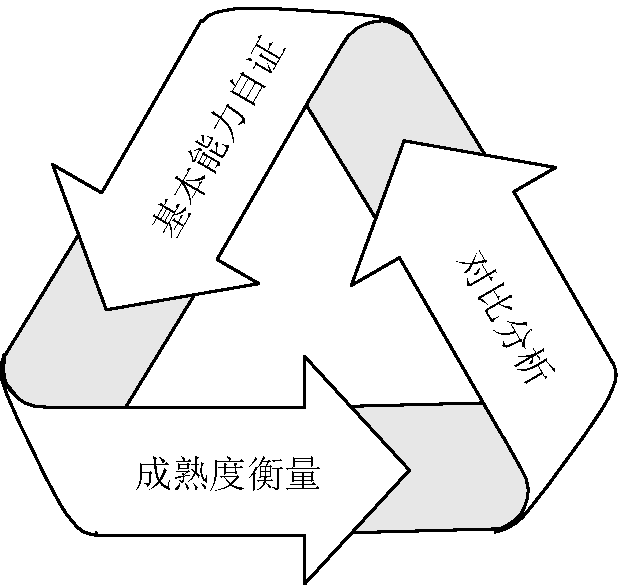
\includegraphics[width=0.4\textwidth]{FIGs/chapter6/assessment.pdf} %中括号中的参数是设置图片充满文档的大小,你也可以使用小数来缩小图片的尺寸。
    \caption{评估体系} %caption是用来给图片加上图题的
    \label{assessment} %这是添加标签,方便在文章中引用图片。
\end{figure}%figure环境

由于在本机环境下搭建Cello会出现诸多问题, 如文件挂载权限、编译等, 所以本文准备了两套测试环境。本文首先在本地环境进行功能方面的测试, 本地机器为MacBook Pro, 并采用Docker for Desktop搭建的单节点Kubernetes充当集群环境; 其次, 在第\ref{section: tool_comparison}节中, 为顺利运行对比工具Cello, 本文利用云主机Ubuntu 18.04搭建Minikube充当集群环境。上述两种环境具体配置如表\ref{computer}所示。

{\footnotesize
\begin{longtable}[h]{m{40pt} m{100pt} m{100pt}}
    \caption[配置详情]{配置详情} \label{computer} \\
        \toprule    
        \textbf{环境} & \textbf{配置项目} & \textbf{配置详情} \\
        \hline
        \multirow{2}*{\parbox[c]{40pt}{本机环境}}    
        & Docker for Desktop&Version 4.7.0\\     
        & Kubernetes&v1.22.5\\
        \hline
        \multirow{3}*{\parbox[c]{40pt}{云主机}} 
        & Docker & Community 20.10.13 \\
        & minikube & v1.25.2 \\
        & Kubernetes & v1.23.3 \\
        \bottomrule 
    \end{longtable} 
}


\section{基本能力自证}\label{section: tool_test}

\subsection{案例研究}

本小节主要以案例研究的方式对原型工具进行功能性测试。如图\ref{fabric_net}所示, 本节将以搭建最经典、简单的HF网络案例的方式针对\ref{section: requirement}节的用例进行完整的功能测试。测试重点针对于Ca、Peer、Orderer启动、创建通道、部署链码、调用的全部过程,验证HF网络启动及链码部署的正确性。

\begin{figure}[h] %figure环境,h默认参数是可以浮动,不是固定在当前位置。如果要不浮动,你就可以使用大写float宏包的H参数,固定图片在当前位置,禁止浮动。
    \centering %使图片居中显示
    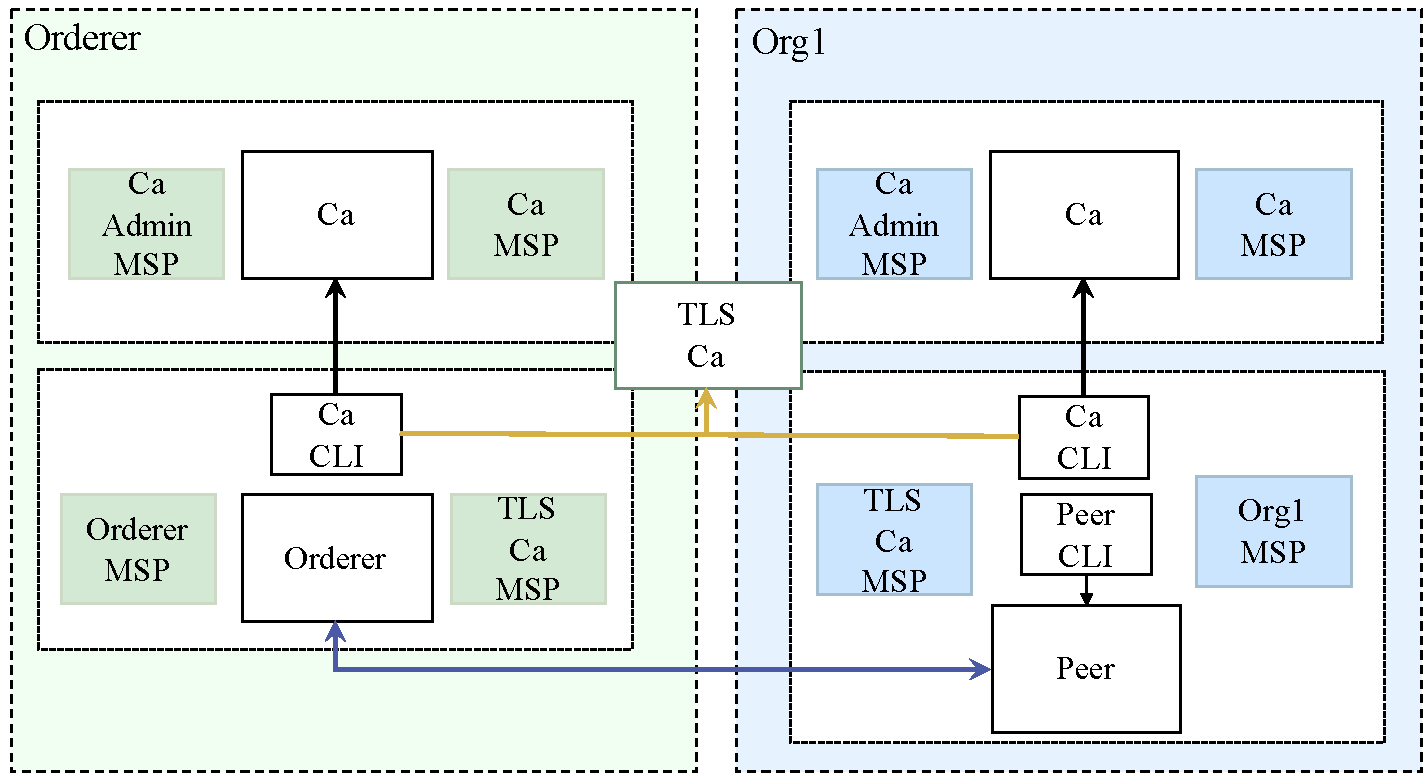
\includegraphics[width=1.0\textwidth]{FIGs/chapter6/fabric_net.pdf} %中括号中的参数是设置图片充满文档的大小,你也可以使用小数来缩小图片的尺寸。
    \caption{测试网络} %caption是用来给图片加上图题的
    \label{fabric_net} %这是添加标签,方便在文章中引用图片。
\end{figure}%figure环境

\textbf{前置条件:}原型工具首先将编写好的HF网络各节点的CRD注入Kubernetes。注入的CRD可以通过原生kubectl命令进行管理。如图\ref{crdresult}所示为部署之后的结果, 已经将Ca、Peer、Orderer和链码的CRD部署入集群。

\begin{figure}[h] %figure环境,h默认参数是可以浮动,不是固定在当前位置。如果要不浮动,你就可以使用大写float宏包的H参数,固定图片在当前位置,禁止浮动。
    \centering %使图片居中显示
    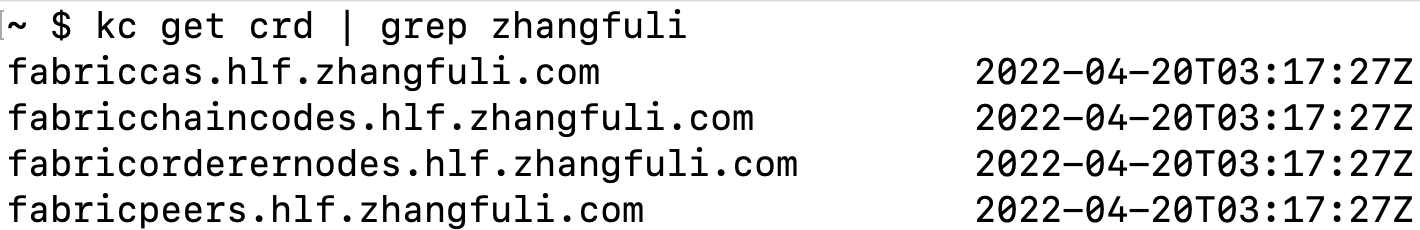
\includegraphics[width=1.0\textwidth]{FIGs/chapter6/crds.png} %中括号中的参数是设置图片充满文档的大小,你也可以使用小数来缩小图片的尺寸。
    \caption{CRD部署结果} %caption是用来给图片加上图题的
    \label{crdresult} %这是添加标签,方便在文章中引用图片。
\end{figure}%figure环境

\textbf{步骤一:} 如表\ref{org1_test}所示, HF网络管理员首先为org1创建了名为“org1-ca”的Ca节点; 其次, 在org1中创建了名为“org1-peer0”的Peer节点,并利用链外存储CouchDB作为账本存储单元。如图\ref{testcase1result}所示为测试结果。

{\footnotesize
\begin{longtable}[h]{m{45pt} m{45pt} m{180pt} m{50pt} m{20pt}}
    \caption[创建Org1测试用例]{Org1测试用例} \label{org1_test}\\
        \toprule  
        \textbf{用例编号}&\textbf{测试编号}&\textbf{用户输入}&\textbf{预期结果}&\textbf{实际}\\
        \hline
        UC-Ca & TC1.1 & 创建名为org1-ca的Ca节点 & 成功启动Ca & 通过 \\
        \hline
        UC-Peer & TC1.2 & 创建名为org1-peer0的Peer节点, 其拥有外部存储CouchDB, 所属于Org1MSP & 成功启动Peer节点 & 通过 \\
        \bottomrule
    \end{longtable} 
}

\begin{figure}[h] %figure环境,h默认参数是可以浮动,不是固定在当前位置。如果要不浮动,你就可以使用大写float宏包的H参数,固定图片在当前位置,禁止浮动。
    \centering %使图片居中显示
    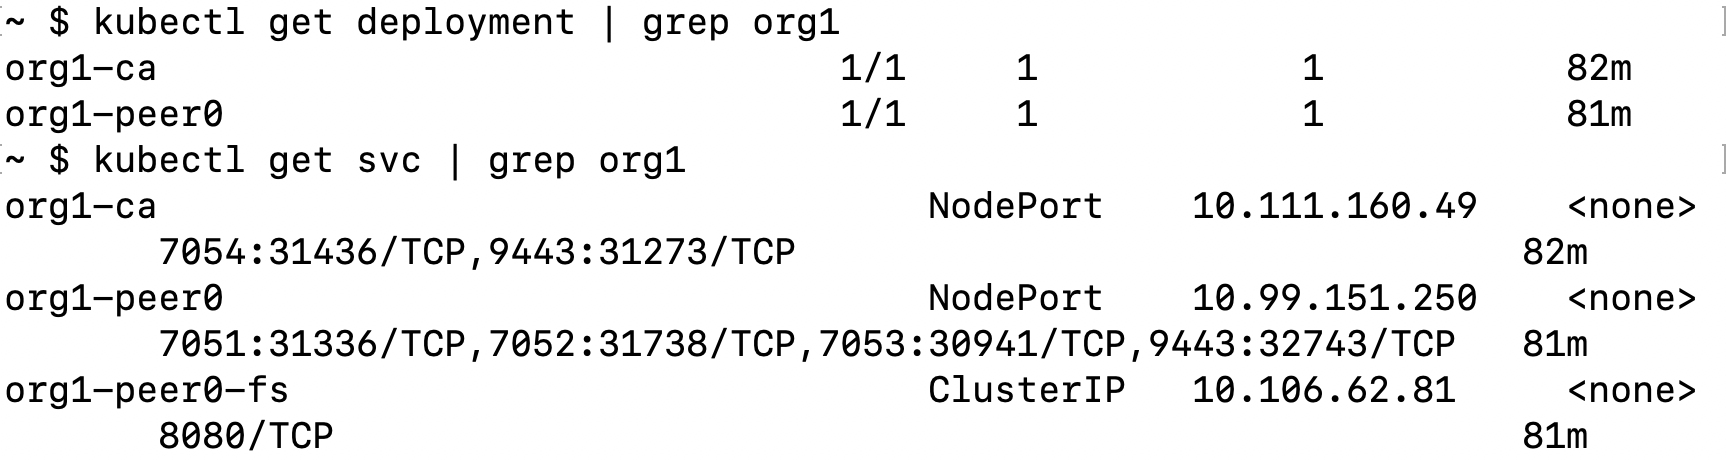
\includegraphics[width=0.9\textwidth]{FIGs/chapter6/peer.png} %中括号中的参数是设置图片充满文档的大小,你也可以使用小数来缩小图片的尺寸。
    \caption{创建Org1测试结果} %caption是用来给图片加上图题的
    \label{testcase1result} %这是添加标签,方便在文章中引用图片。
\end{figure}%figure环境

\textbf{步骤二:} 如表\ref{orderer_test}所示, HF网络管理员需要首先为OrdererMSP创建名为“ord-ca”的Ca节点; 其次, 在OrdererMSP中创建了名为“ord-node1”的Peer节点。如图\ref{testcase2result}所示为测试结果, 原型工具可以为HF网络管理员创建Orderer组织的Ca与Orderer节点, 其中包含但不限于Deployment、Service、Pod、Secret等。

{\footnotesize
\begin{longtable}[h]{m{45pt} m{45pt} m{180pt} m{50pt} m{20pt}}
    \caption[创建Orderer测试用例]{创建Orderer测试用例} \label{orderer_test}\\
        \toprule  
        \textbf{用例编号}&\textbf{测试编号}&\textbf{用户输入}&\textbf{预期结果}&\textbf{实际}\\
        \hline
        UC-Ca & TC2.1 & 创建名为ord-ca的Ca节点 & 成功启动Ca & 通过 \\
        \hline
        UC-Orderer & TC2.2 & 创建名为ord-node1的Orderer节点, 所属于OrdererMSP & 成功启动Orderer节点 & 通过 \\
        \bottomrule
    \end{longtable} 
}

\begin{figure}[h] %figure环境,h默认参数是可以浮动,不是固定在当前位置。如果要不浮动,你就可以使用大写float宏包的H参数,固定图片在当前位置,禁止浮动。
    \centering %使图片居中显示
    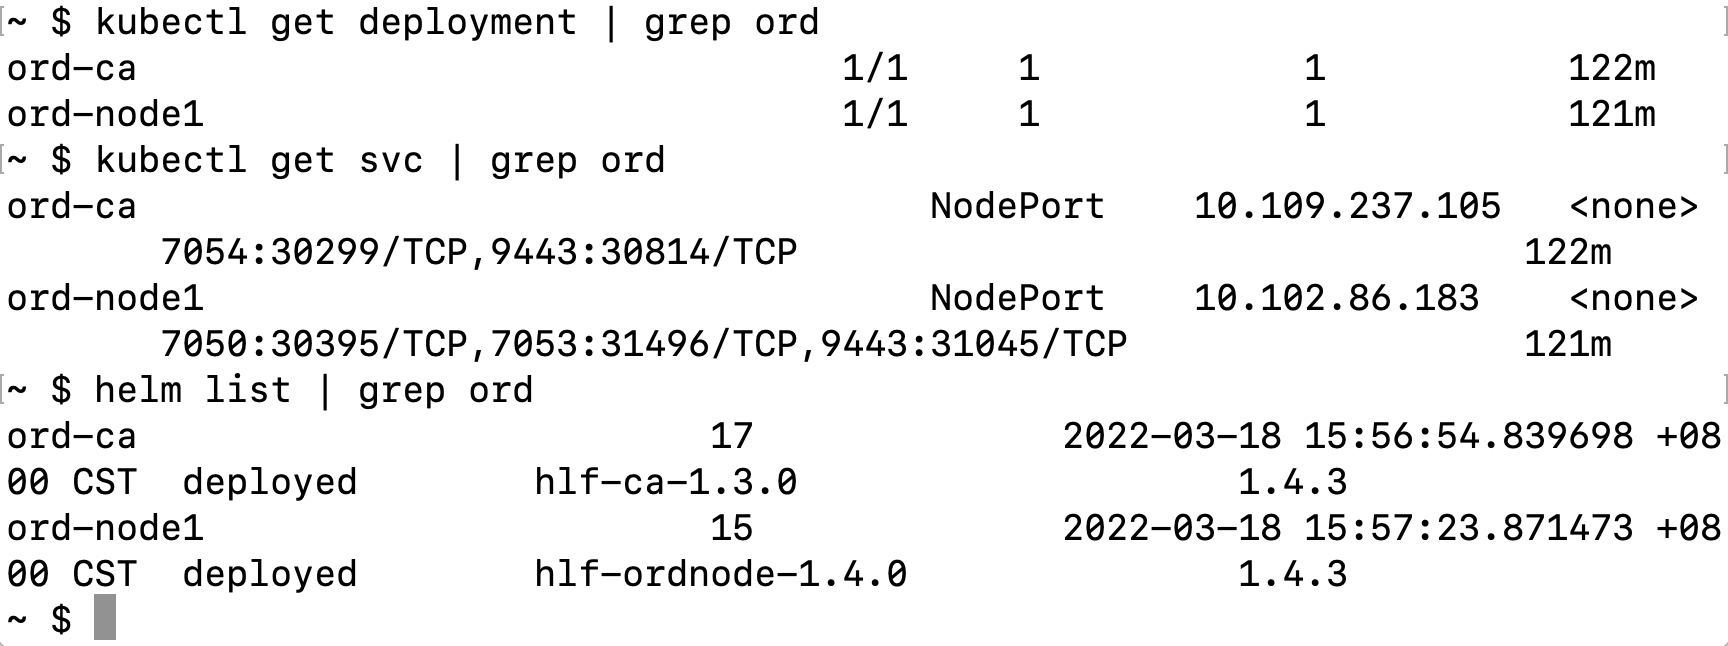
\includegraphics[width=0.9\textwidth]{FIGs/chapter6/orderer.png} %中括号中的参数是设置图片充满文档的大小,你也可以使用小数来缩小图片的尺寸。
    \caption{创建Orderer测试结果} %caption是用来给图片加上图题的
    \label{testcase2result} %这是添加标签,方便在文章中引用图片。
\end{figure}%figure环境

\textbf{步骤三:} 如表\ref{reg_enroll_test}所示, HF网络管理员需要为OrdererMSP以及Org1注册并登记若干用户, 并将用户的证书密钥信息导到Yaml文件中。表中仅展示在Orderer中注册用户, Org1中步骤相似, 注册名为peeruser的用户。测试结果表明, 可以成功将用户及OrdererMSP信息导出。

{\footnotesize
\begin{longtable}[h]{m{45pt} m{45pt} m{180pt} m{50pt} m{20pt}}
    \caption[注册、登记用户测试用例]{注册、登记用户测试用例} \label{reg_enroll_test}\\
        \toprule  
        \textbf{用例编号}&\textbf{测试编号}&\textbf{用户输入}&\textbf{预期结果}&\textbf{实际}\\
        \hline
        UC-Ca & TC3.1 & 为OrdererMSP注册名为ordereruser的用户, 其密码为ordererpw & 成功注册 & 通过 \\
        \hline
        UC-Ca & TC3.2 & 输入用户名密码, 为ordereruser用户登记 & 成功登记,输出证书文件 & 通过 \\
        \bottomrule
    \end{longtable} 
}

\textbf{步骤四:} 如表\ref{channel_test}所示, HF开发人员需要在新创建的HF网络上创建通道, 并初始化该通道内的创世区块。当通道被创建完成之后, 需要将在该通道内进行交易的Orderer、Peer加入该通道。最后, HF开发人员可以指定锚节点并查看通道的高度。如图\ref{channel_test_result}所示为测试结果, 展示了新创建的通道的高度。

{\footnotesize
\begin{longtable}[h]{m{45pt} m{45pt} m{180pt} m{50pt} m{20pt}}
    \caption[创建通道测试用例]{创建通道测试用例} \label{channel_test}\\
        \toprule  
        \textbf{用例编号}&\textbf{测试编号}&\textbf{用户输入}&\textbf{预期结果}&\textbf{实际}\\
        \hline
        UC-Chan & TC4.1 & 选择OrdererMSP为排序组织在Org1MSP上创建通道 & 成功创建通道 & 通过 \\
        \hline
        UC-Chan & TC4.2 & 在通道内创建创世节点 & 成功创建创世节点 & 通过 \\
        \hline
        UC-Orderer & TC4.2 & 将ord-node1加入通道 & 加入成功 & 通过 \\
        \hline
        UC-Peer & TC4.3 & 将org1-peer0加入通道 & 加入成功 & 通过 \\
        \hline
        UC-Chan & TC4.4 & 指定锚节点 & 指定成功 & 通过 \\
        \hline
        UC-Chan & TC4.5 & 查看通道高度 & 查看成功 & 通过 \\
        \bottomrule
    \end{longtable} 
}

\begin{figure}[h] %figure环境,h默认参数是可以浮动,不是固定在当前位置。如果要不浮动,你就可以使用大写float宏包的H参数,固定图片在当前位置,禁止浮动。
    \centering %使图片居中显示
    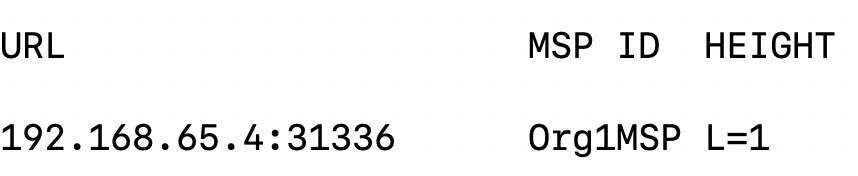
\includegraphics[width=0.6\textwidth]{FIGs/chapter6/channel.png} %中括号中的参数是设置图片充满文档的大小,你也可以使用小数来缩小图片的尺寸。
    \caption{查看通道高度测试结果} %caption是用来给图片加上图题的
    \label{channel_test_result} %这是添加标签,方便在文章中引用图片。
\end{figure}%figure环境

\textbf{步骤五:} 如表\ref{chaincode_test}所示, 为测试通道内所有的参与节点按照链码的合同规则执行, HF开发人员需要在新创建的通道内安装官方提供的asset\footnotemark[1]\footnotetext[1]{\href{https://github.com/hyperledger/fabric-samples/blob/main/asset-transfer-basic/chaincode-go/chaincode/smartcontract.go}{asset链码}}链码, 安装完链码之后, 需要对其进行审批、提交。最后, HF开发人员可以调用链码接口对其进行初始化、查询等一系列操作。如图\ref{chaincode_test_result}所示仅为调用测试结果, 第\ref{section: smart_contract_microservice_test}节已经证明了智能合约微服务化的可行性。

{\footnotesize
\begin{longtable}[h]{m{45pt} m{45pt} m{180pt} m{50pt} m{20pt}}
    \caption[创建通道测试用例]{创建通道测试用例} \label{chaincode_test}\\
        \toprule  
        \textbf{用例编号}&\textbf{测试编号}&\textbf{用户输入}&\textbf{预期结果}&\textbf{实际}\\
        \hline
        UC-CC & TC5.1 & 安装链码并指定语言、label & 安装成功 & 通过 \\
        \hline
        UC-CC & TC5.2 & 查询已经安装的链码 & 查询成功 & 通过 \\
        \hline
        UC-CC & TC5.3 & 审批链码, 并提供链码ID以及策略 & 审批成功 & 通过 \\
        \hline
        UC-CC & TC5.4 & 提交链码, 并提供链码ID以及策略 & 指定成功 & 通过 \\
        \hline
        UC-CC & TC5.5 & 调用链码, 并提供链码调用函数 & 调用成功 & 通过 \\
        \bottomrule
    \end{longtable} 
}

\begin{figure}[h] %figure环境,h默认参数是可以浮动,不是固定在当前位置。如果要不浮动,你就可以使用大写float宏包的H参数,固定图片在当前位置,禁止浮动。
    \centering %使图片居中显示
    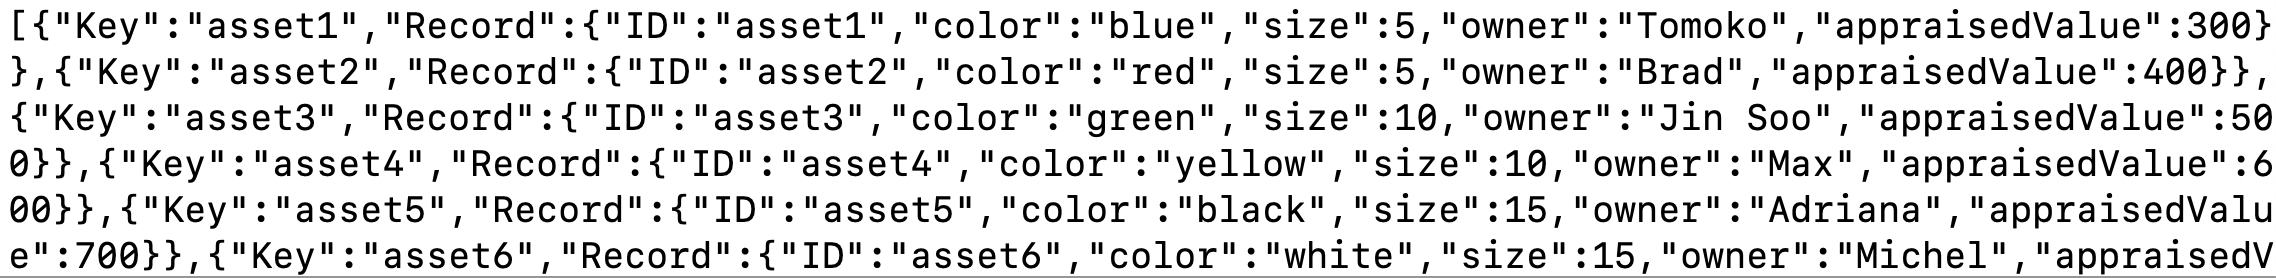
\includegraphics[width=1.0\textwidth]{FIGs/chapter6/chaincode.png} %中括号中的参数是设置图片充满文档的大小,你也可以使用小数来缩小图片的尺寸。
    \caption{查询链码} %caption是用来给图片加上图题的
    \label{chaincode_test_result} %这是添加标签,方便在文章中引用图片。
\end{figure}%figure环境


经过上述步骤1-5, 最终的网络节点状态如图\ref{fabric_result}所示, 本文搭建了一个单Orderer以及单Org、单Peer的经典HF网络, 并分别为Orderer、以及Peer组织搭配Ca证书认证。在搭建了基本的网络之后, 分别为Orderer、Peer注册并登记用户, 最后在组织Org中搭建了一个通道并成功安装调用并链码。由案例分析的结果可知, 本文的区块链云化框架及原型工具能够成功搭建HF网络节点并能够正确地部署、运行链码。

\begin{figure}[h] %figure环境,h默认参数是可以浮动,不是固定在当前位置。如果要不浮动,你就可以使用大写float宏包的H参数,固定图片在当前位置,禁止浮动。
    \centering %使图片居中显示
    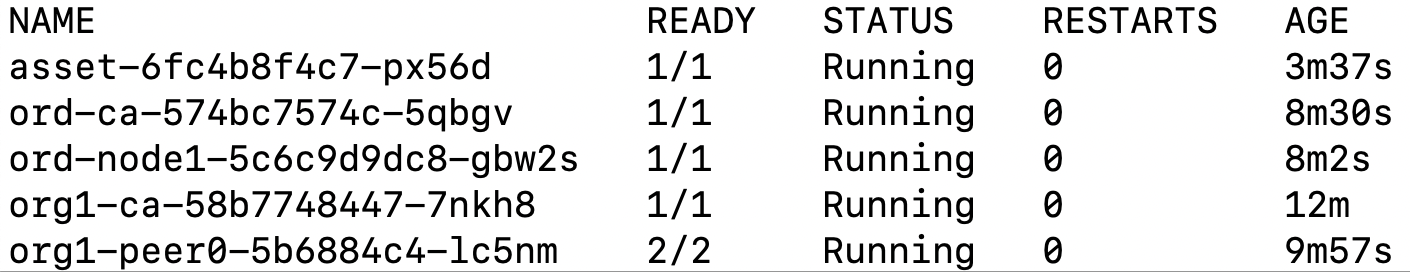
\includegraphics[width=1.0\textwidth]{FIGs/chapter6/fabric_result.png} %中括号中的参数是设置图片充满文档的大小,你也可以使用小数来缩小图片的尺寸。
    \caption{网络节点状态} %caption是用来给图片加上图题的
    \label{fabric_result} %这是添加标签,方便在文章中引用图片。
\end{figure}%figure环境


\subsection{架构评估}

在软件工程中, 常见的评估软件体系结构的方法有Software Architecture Analysis Method(SAAM)、Architecture Trade-off Analysis Method(ATAM), 以上都是基于场景的质量属性评估方法\cite{ionita2002scenario}。SAAM相较于ATAM而言其结构以及评估过程相对简单, 需要准备的工作较少并且SAAM适用于对软件最终版本的评估\cite{huhonglei2004}。本文首先对第\ref{section: framework_characteristics}节所涉及到的设计原则的描述映射到对应的质量属性, 然后采取SAAM方法对其进行评估。

在SAAM评估方法开始之前, 本文邀请了4位熟悉HF基本概念及网络搭建流程的软件开发工程师分别两两扮演HF网络管理员、HF开发人员, 1位熟悉Kubernetes操作的集群运维工程师扮演集群管理员, 以上5位分别为本次SAAM评估方法的风险承担者。本节实施SAAM评估方法涉及以下步骤:

\textbf{1. 场景开发: }所有的风险承担者通过头脑风暴的方式, 提出反应自己需求的场景, 产出结果见步骤3。

\textbf{2. 软件架构描述: }本文详细的为各位风险承担者介绍面向Hyperledger Fabric的区块链云化框架及其原型工具, 包括框架设计理念与原理、原型工具功能和工具实现细节。

\textbf{3. 场景分类: }在这个过程中, 如表\ref{saam_step3}所示, 本文对步骤1所产出的场景进行分类并设定优先级。同时, 在分析时根据场景是否需要修改特定的体系结构把场景分为直接场景与间接场景。

{\footnotesize
\begin{longtable}[h]{m{20pt} m{60pt} m{90pt} m{40pt} m{40pt} m{40pt} m{30pt}}
    \caption[场景分类结果]{场景分类结果} \label{saam_step3}\\
        \toprule  
        \textbf{编号}&\textbf{风险承担者}&\textbf{场景描述}&\textbf{设计原则}&\textbf{质量属性}&\textbf{场景分类}&\textbf{优先级}\\
        \hline
        T1&  HF网络管理员 & 命令式启停HF网络中的任意节点 & 简单易用  & 功能需求 & 直接需求 &  高 \\
        \hline
        T2&  HF网络管理员 & 命令创建HF网络用户 & 简单易用 & 功能需求 & 直接需求 &  高 \\
        \hline
        T3&  HF开发人员 & 命令式创建通道 & 简单易用 & 功能需求 & 直接需求 &  高 \\
        \hline
        T4&  HF开发人员 & 持续交付部署链码 & 简单易用 & 功能需求 & 直接需求 &  高 \\
        \hline
        T5&  HF开发人员 & 命令式操作链码 & 简单易用 & 功能需求 & 直接需求 &  高 \\
        \hline
        T6&  HF网络管理员 \newline HF开发人员 & 能在30min内启动完整网络 & 简单易用 & 易用性 & 间接需求 &  高 \\
        \hline
        T7&  HF网络管理员 & 扩容HF节点资源 & 灵活扩展 & 可扩展性 & 间接需求 &  中 \\
        \hline
        T8&  HF网络管理员 & 扩容账本存储单元 & 灵活扩展 & 可扩展性 & 间接需求 &  高 \\
        \hline
        T9&  HF开发人员 & 保存用户密钥 & 安全可靠 & 安全性 & 间接需求 &  高 \\
        \hline
        T10&  HF开发人员 & 操作网络时需要身份认证 & 安全可靠 & 安全性 & 间接需求 &  高 \\
        \hline    
        T11&  k8s管理员 & HF网络与其他集群程序进行隔离 & 安全可靠 & 安全性 & 间接需求 &  高 \\
        \hline
        T12&  k8s管理员 & Operator限定管理HF网络节点 & 安全可靠 & 安全性 & 间接需求 &  高 \\
        \hline
        T13&  HF网络管理员 \newline HF开发人员 & 良好异常反馈机制 & 安全可靠 & 可靠性 & 间接需求 &  高 \\
        \hline
        T14&  HF网络管理员 \newline HF开发人员 & HF网络节点的全面监控能力 & 可视运维 & 可靠性 & 间接需求 &  高 \\
        \hline
        T15&  HF网络管理员 \newline HF开发人员 & Operator在不同云平台之间迁移的便捷性 & 云链结合 & 可移植性 & 间接需求 &  中 \\
        \bottomrule
    \end{longtable} 
}

\textbf{4. 场景评估: }这个过程重点针对间接场景, 并对其进行评估。针对直接场景, 第\ref{section: tool_test}节已经对其进行了较为全面的功能性测试。

简单易用, 本文同时邀请了这5位风险承担者对本文的原型工具进行易用性测试。为了排除网络的影响,
本文提前下载好原型工具搭建HF网络所需要的Docker镜像。在介绍了本工具的基本原理以及命令行的基本使用方法后, 5位风险承担者分别独立自行搭建不同规格的HF网络, 最终5位风险承担者都能够在30分钟内学习并掌握原型工具的使用方法。


\begin{figure}[h] %figure环境,h默认参数是可以浮动,不是固定在当前位置。如果要不浮动,你就可以使用大写float宏包的H参数,固定图片在当前位置,禁止浮动。
    \centering %使图片居中显示
    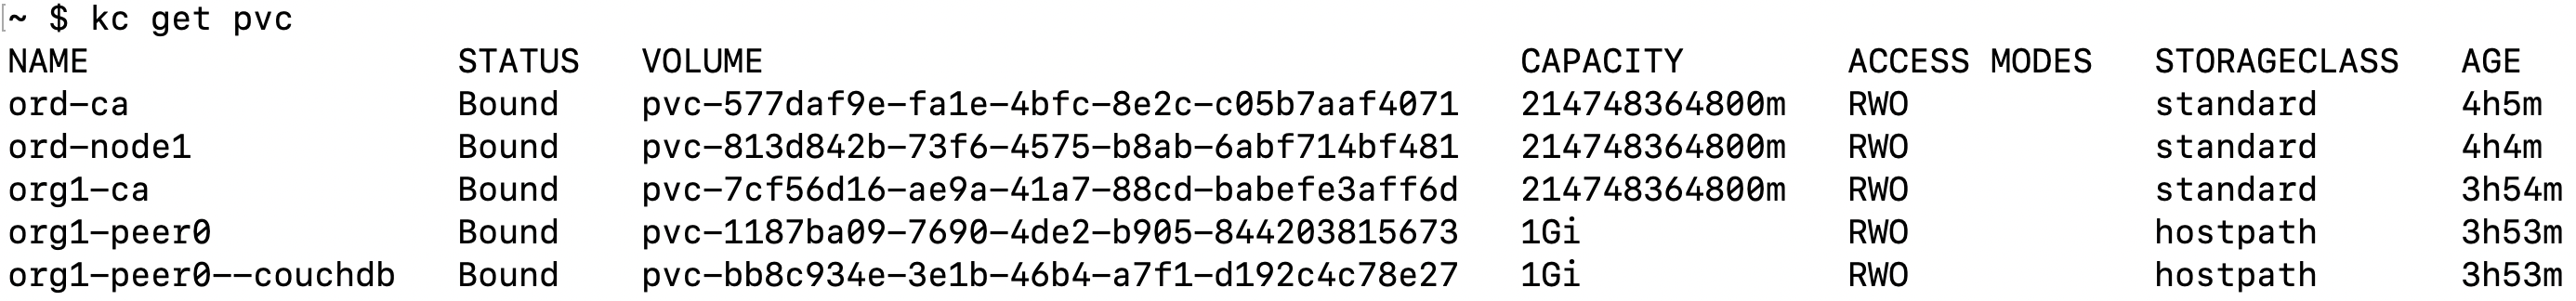
\includegraphics[width=1.0\textwidth]{FIGs/chapter6/db.png} %中括号中的参数是设置图片充满文档的大小,你也可以使用小数来缩小图片的尺寸。
    \caption{网络存储状态} %caption是用来给图片加上图题的
    \label{db} %这是添加标签,方便在文章中引用图片。
\end{figure}%figure环境

灵活扩展, 在HF网络节点资源方面, 由于HF网络节点的CR中配置了HF网络节点运行态时所需的资源(CPU、内存)大小, 所以当对节点CR进行修改时, Controller会监听到CR的变化并更新运行中节点Deployment的资源大小。在数据存储的可扩展性方面,如图\ref{db}所示, 原型工具为每个HF网络中的工作节点设置了专属存储单元。每个存储单元配置专属的PVC管理, HF网络管理员可以不仅可以通过修改节点的CR进行扩容, 可以直接在Kubernetes中对PVC进行动态扩容。值得注意的是, 由于存储单元PVC扩容依赖于StorageClass, 当前只有AWS-EBS、GCE-PD、Azure磁盘、Azure文件、Glusterfs、Cinder、Portworx和Ceph RBD数据卷插件才能支撑数据扩容操作。


安全可靠, 原型工具通过可以以文件形式导出HF网络登记用户产生的密钥信息, 并可以通过Secret进行保存。当这些用户操作HF网络时, 原型工具会要求提供对应的密钥文件作为身份认证的方式。同时, 原型工具将所有的HF资源放在同一命名空间下, 并通过RBAC为该命名空间提供了两种类型的角色。当集群其他用户对已经部署的HF网络节点拥有超越权限的操作时, 原型工具会提示并不进行相关操作。在可靠性方面, 本文在使用原型工具搭建HF网络过程中有意输入错误的命令行参数, 输入不正确的密钥文件等, 原型工具都能在1s内给出参数的异常情况; 同时, 原型工具能够有效利用Prometheus监控体系对工具本身以及HF网络的所有节点、链码以及DB进行监控, 如图\ref{monitoring}展示了利用Prometheus与Grafana对Ca Resource进行监控的画面, 图中展示了Ca CPU的使用情况。在搭建完HF网络之后, 原型工具在两周内仅崩溃1次, 且能通过日志以及Prometheus的告警设置在5分钟内进行恢复。

\begin{figure}[h] %figure环境,h默认参数是可以浮动,不是固定在当前位置。如果要不浮动,你就可以使用大写float宏包的H参数,固定图片在当前位置,禁止浮动。
    \centering %使图片居中显示
    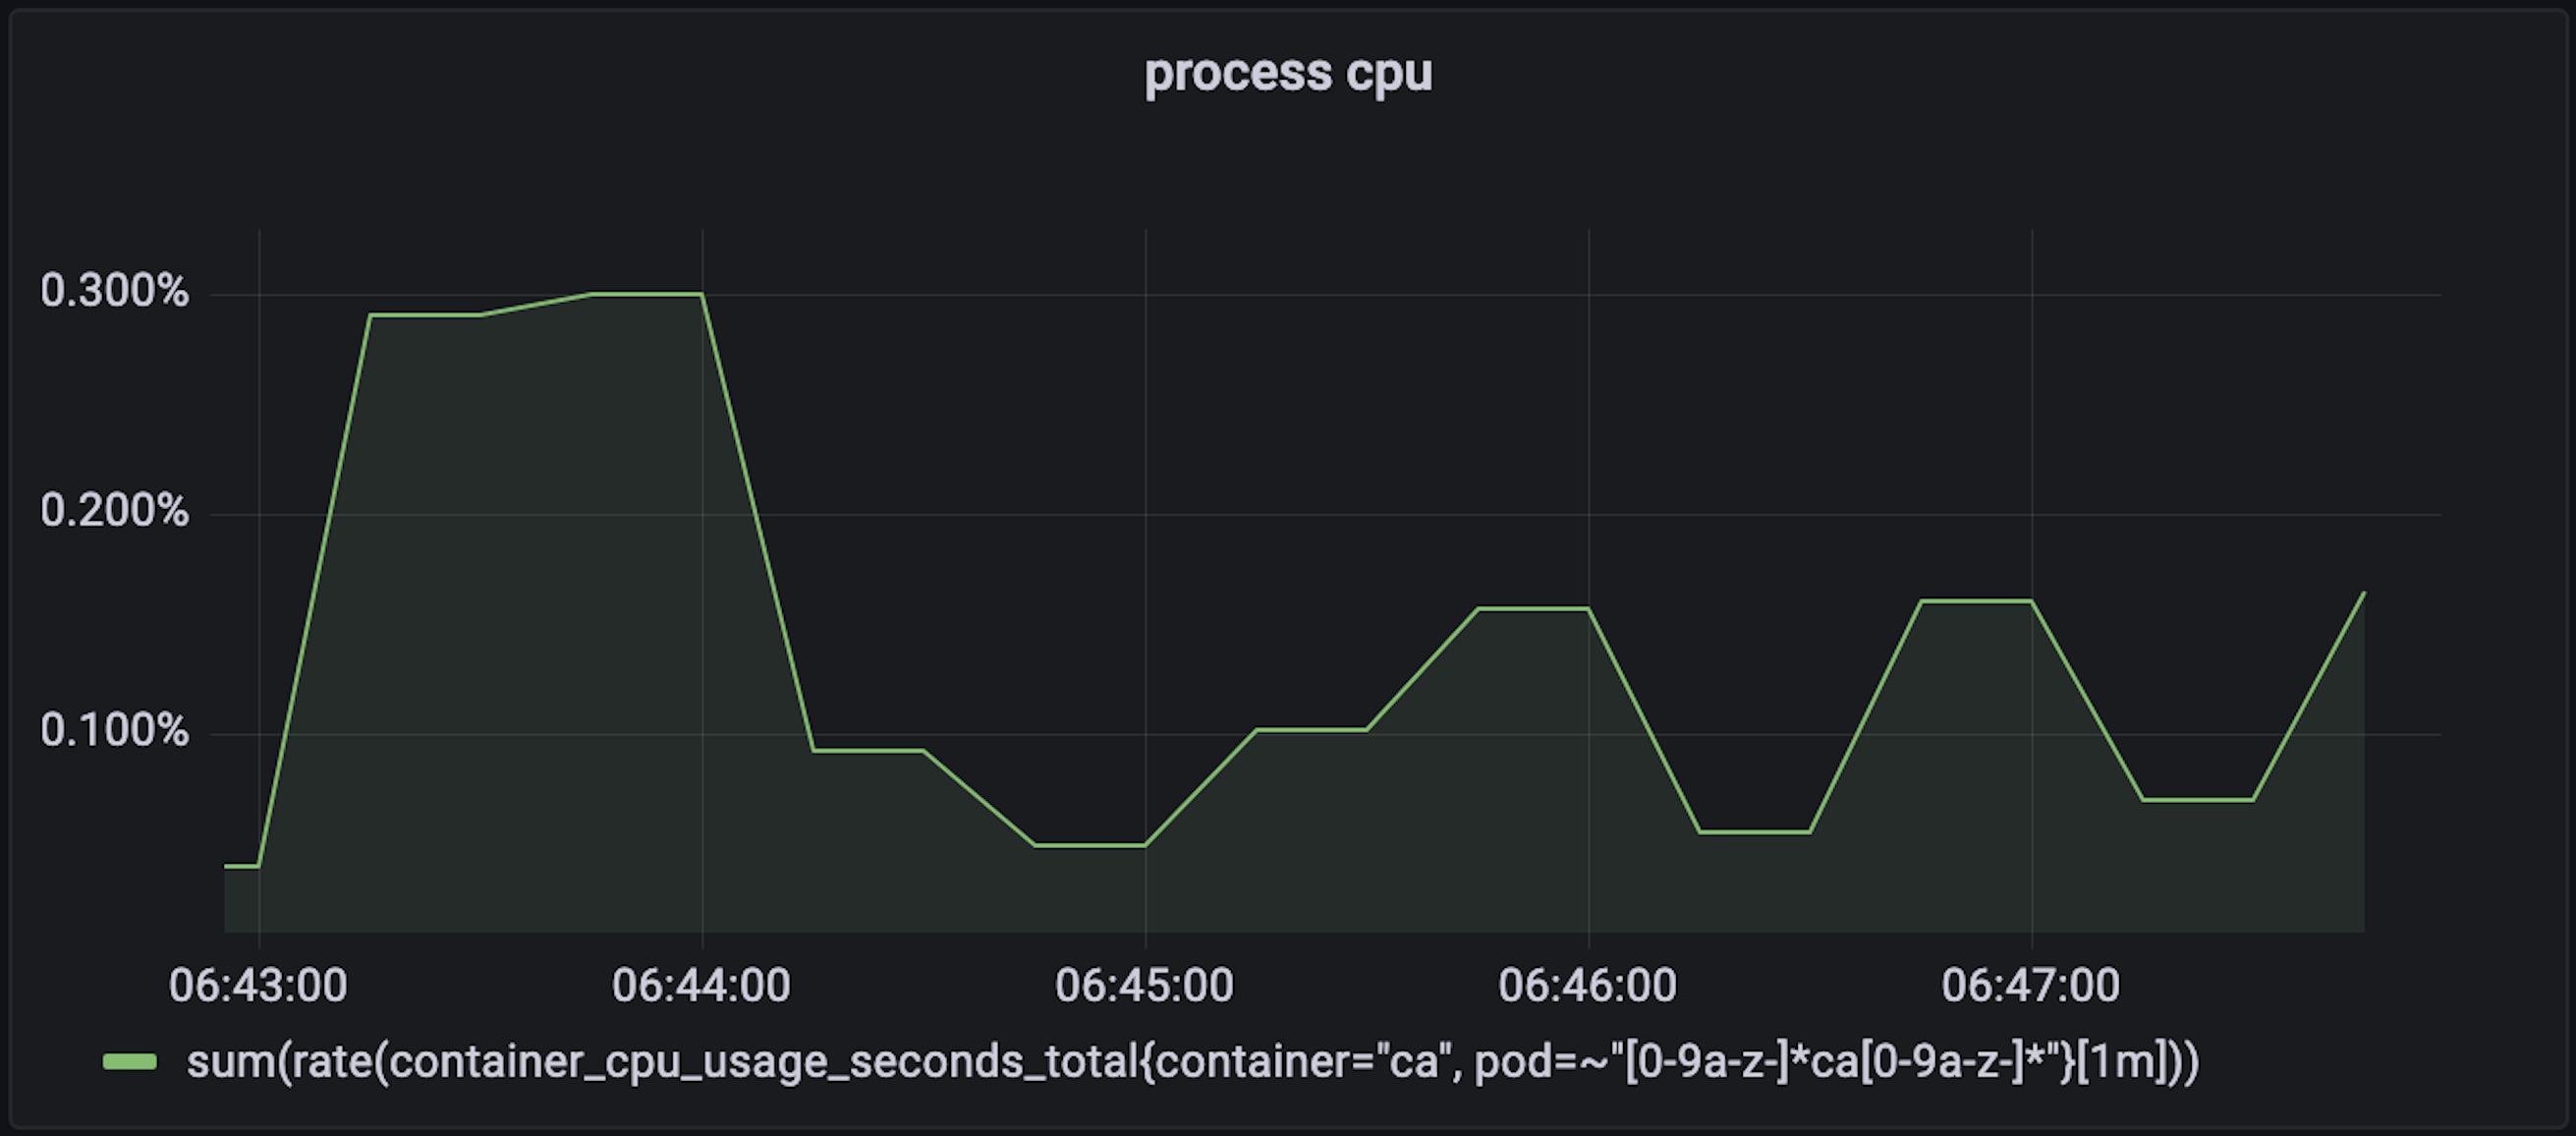
\includegraphics[width=0.9\textwidth]{FIGs/chapter6/ca_cpu.png} %中括号中的参数是设置图片充满文档的大小,你也可以使用小数来缩小图片的尺寸。
    \caption{Ca CPU监控图} %caption是用来给图片加上图题的
    \label{monitoring} %这是添加标签,方便在文章中引用图片。
\end{figure}%figure环境

云链结合, 重点是在可移植性下的场景。本文通过Dockerfile将本工具打包成Docker镜像\footnotemark[1]\footnotetext[1]{\href{https://hub.docker.com/repository/docker/zhangfuli/hfoperator}{HFOperator镜像}}, 使用预先打包并经过检验的镜像, 并为该原型工具配备专用的Helm chart, 其中包含有关原型工具构建的所有必要信息, 这样可以以最少的时间部署。结果表明, 原型工具可以通过Helm在支持Kubernetes 1.18版本以上的云平台上运行, 原型平台具备良好的可移植性。

\textbf{5. 总体评估: }本文的原型工具可以有效利用Kubernetes Operator云化策略来提升HF网络节点的易用性、可扩展性、安全性、以及可靠性。


\section{成熟度衡量}

\begin{figure}[h] %figure环境,h默认参数是可以浮动,不是固定在当前位置。如果要不浮动,你就可以使用大写float宏包的H参数,固定图片在当前位置,禁止浮动。
    \centering %使图片居中显示
    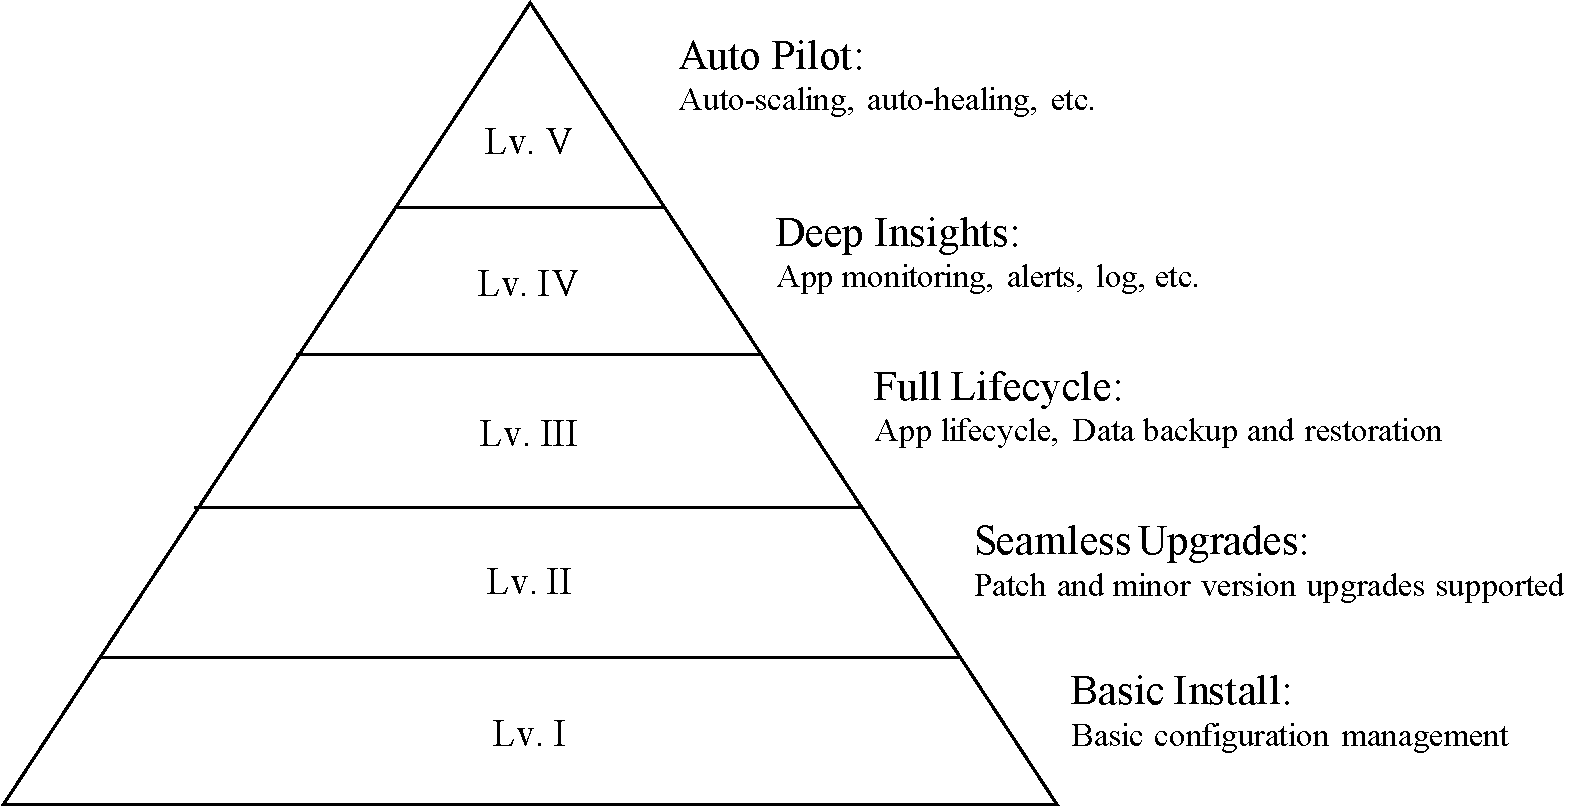
\includegraphics[width=0.95\textwidth]{FIGs/chapter6/maturity.pdf} %中括号中的参数是设置图片充满文档的大小,你也可以使用小数来缩小图片的尺寸。
    \caption{成熟度模型} %caption是用来给图片加上图题的
    \label{maturity} %这是添加标签,方便在文章中引用图片。
\end{figure}%figure环境


如图所示\ref{maturity}, Kubernetes Operator拥有5个成熟度级别的定义\cite{duan2021case}, 其通过定性的方式分析某个Operator应用是否达到了某个级别, 这5个成熟度级别定义如下:

\begin{itemize}[itemindent=2em]
    \item 第一级: Basic Install, 该级是Operator成熟度模型中最基本的级别。在该级中, 用户能够使用CRD对目标程序进行配置和安装;

    \item 第二级: Seamless Upgrades, 在该级别上的Operator能够不丢失数据的升级所管理的工作负载;

    \item 第三级: Full Lifecycle, 是否能达到该级别取决于Operator是否具备生命周期管理和的数据备份、恢复能力。在该级别上的Operator能够备份数据, 并在发生任何数据灾难时从备份数据中恢复数据;

    \item 第四级: Deep Insights, Operator提供监控和报警等功能。在该级别, Operator能够包含所有组件的运行状况指标, 并根据指标配备报警功能;

    \item 第五级: Auto Pilot, 最终级别拥有许多高级功能, 如自动伸缩。Operator可以根据收集到的指标来扩展工作负载。

\end{itemize}

\textbf{Basic Install}

借助于原型工具, 用户能够通过命令行方式一键启停HF网络中任意节点, 而且不需要进行复杂的证书管理。一旦原型工具被部署在Kubernetes网络中, 原型工具就可以对CR以及Helm进行管理, HF网络管理人员可以借助命令行参数的方式进行创建、更新CR以此来创建特定规格的HF网络。 一旦CR进行更新, 原型工具就会将当前状态调整为与指定状态一致。

\textbf{Seamless Upgrades}

在原型工具中, HF网络管理员可以通过修改CR的内容对包括HF网络节点镜像、端口、Host、版本等进行无缝修改。此外, 由于原型工具依赖于链外存储的CouchDB以及外部的Prometheus监控体系, 这两者的升级并不会对原型工具产生严重的负面影响。 

\textbf{Full Lifecycle}

虽然原型工具能够在Mangager中对结合Helm对HF网络进行全生命周期管理, 但目前原型工具目前仍缺少数据备份和恢复的能力。要达到这一能力需要在CR中指定远程备份的数据存储平台, 并在CR中指定数据备份的凭证以及远程备份的链接。同时, 原型工具需要在一定的时间周期内将数据备份到远程的数据存储平台上。

\textbf{Deep Insights}

原型工具利用Prometheus监控体系实现监控与报警的功能, 与此同时, 除了利用Prometheus抓取Pod的基本指标外, CRD中还设定了PodMonitor、ServiceMonitor、CouchDBExporter接口, 可以让Prometheus更全面的抓取HF网络的监控指标。HF网络管理员可以通过Grafna可视化图表查看整体HF网络运行状态, 并且能够根据监控指标创建自定义的告警规则。

\textbf{Auto Pilot}

在Kubernetes中存在两种自动伸缩的插件, 即HPA、VPA。当负载超过一定的阈值时, 就会对其进行伸缩或配置更多的资源。然而在HF网络中, 每个Peer都有记录全部账本的职责, 并且只需要超过51\%的Peer节点保持一致即可, 所以针对于Peer并不需要根据监控进行自我伸缩的能力。在数据存储方面, 随着账本的膨胀, 原型工具可以针对链外存储进行扩容。

综上, 通过定性分析, 本文原型工具利用Operator管理HF网络能够完美的具备第一级、第二级的能力, 在第三级上能够支持全生命周期管理但是对于数据的备份能力依旧是存在欠缺, 借助Prometheus实现了第四级的监控, 对于自动伸缩方面支持资源及数据层面的扩展, 所以本文原型工具基本满足5层成熟度模型的功能。

\section{对比分析} \label{section: tool_comparison}

除上述通过定性分析的手段对原型工具进行评估外, 本文选取了Hyperledger官方推出的BaaS平台Cello进行定量的对比分析。本文重点关注的是对HF网络节点的云化问题, 所以需要在网络部署时间与链码交付时间上对Cello以及原型工具进行对比。

本文在云主机环境下拉取Cello的release-0.9.0-h3c并进行打包构建以及运行。Cello通过图形化的Cello Operator进行主机绑定、组织管理、网络管理以及用户管理。操作Cello Operator的就是HF网络管理员, 管理员首先在主机管理中添加主机, 主机就是Cello将要部署的目标Docker或者Kubernetes环境, 然后再依次创建组织并启动网络, 整个过程全都通过图形化界面的方式完成。

% 如图\ref{cello}所示,
% \begin{figure}[h] %figure环境,h默认参数是可以浮动,不是固定在当前位置。如果要不浮动,你就可以使用大写float宏包的H参数,固定图片在当前位置,禁止浮动。
%     \centering %使图片居中显示
%     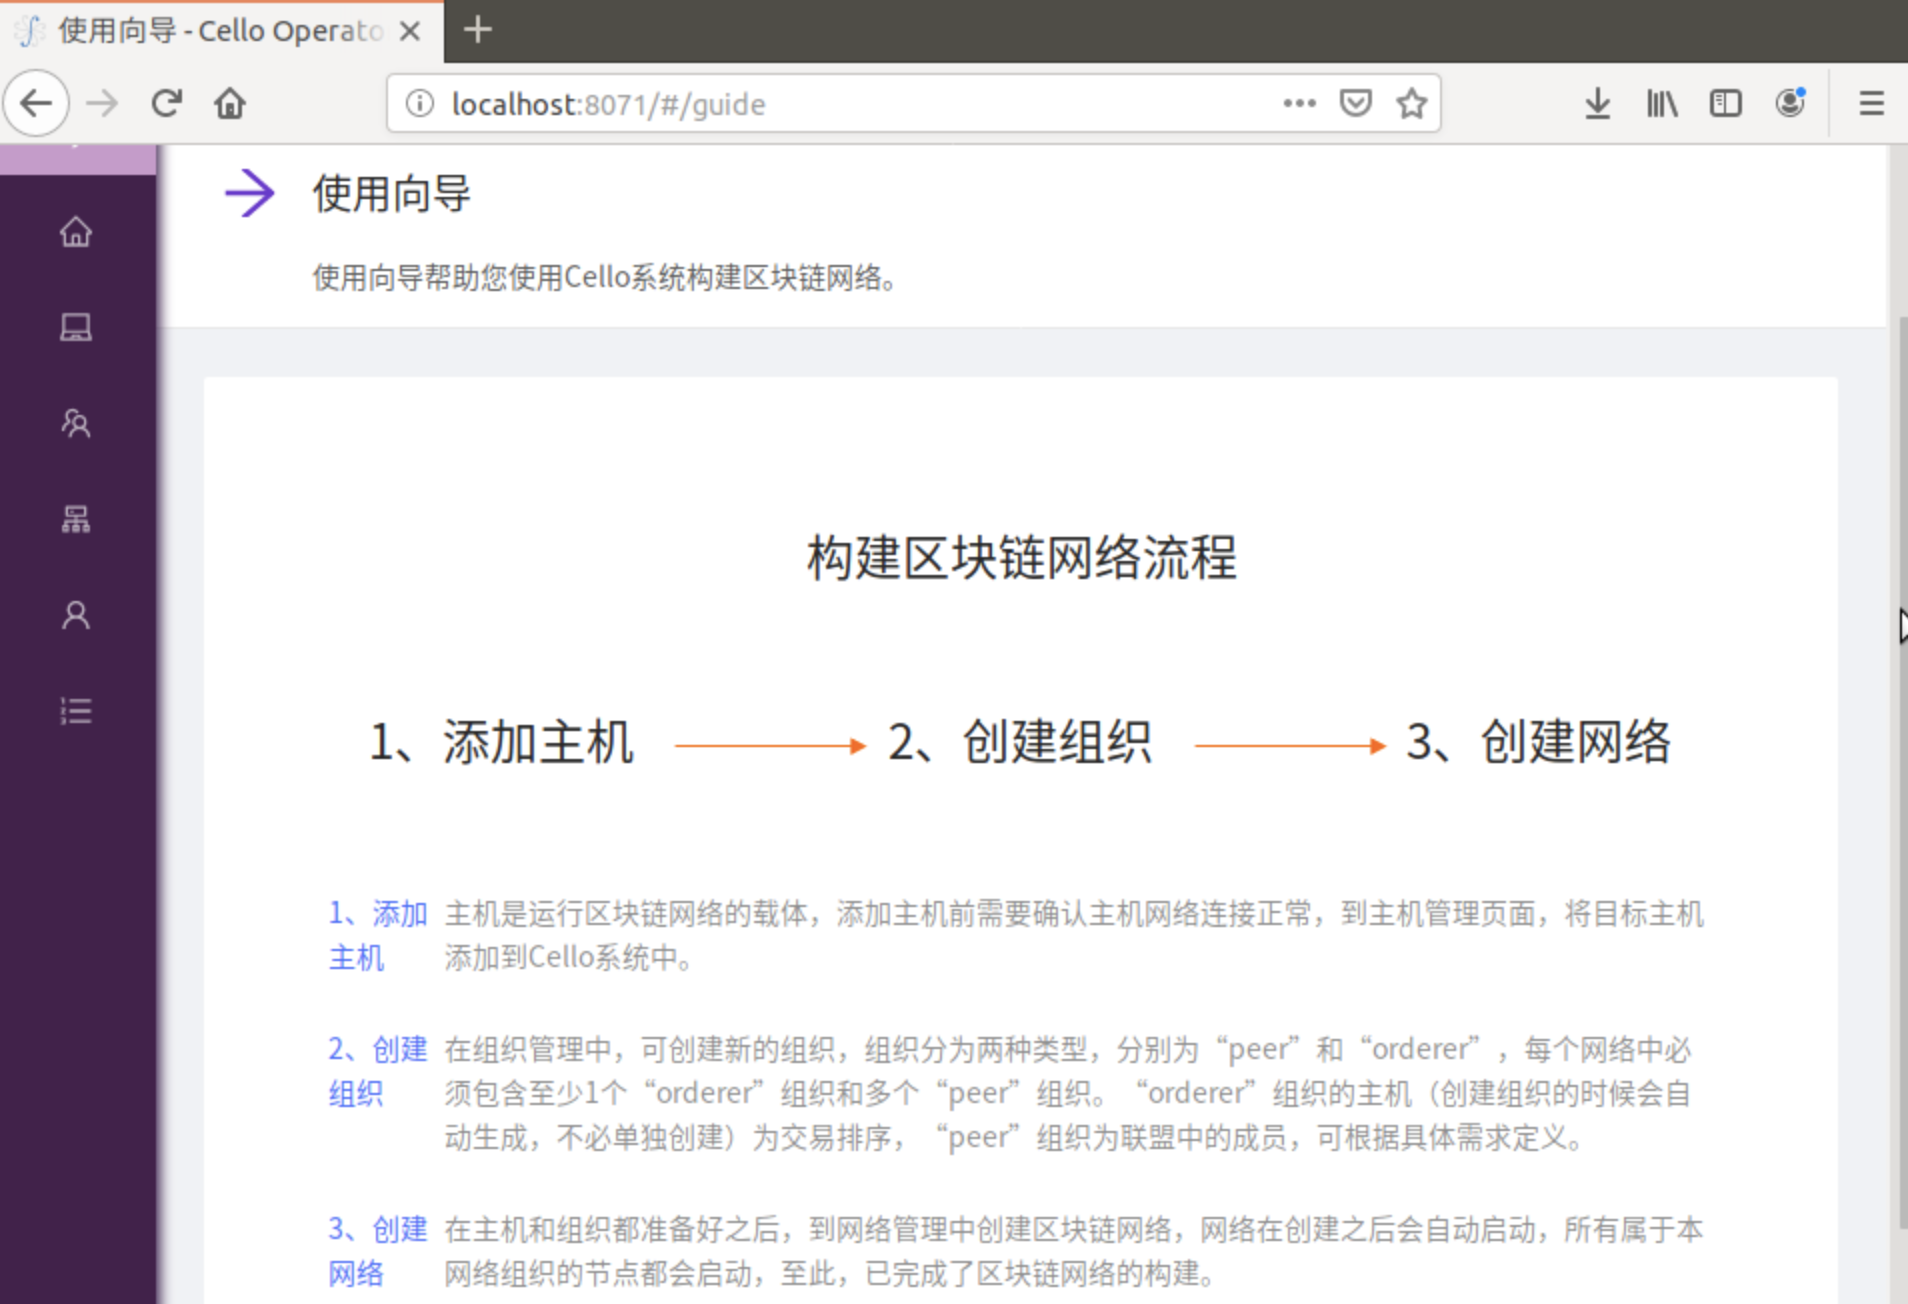
\includegraphics[width=0.95\textwidth]{FIGs/chapter6/cello.png} %中括号中的参数是设置图片充满文档的大小,你也可以使用小数来缩小图片的尺寸。
%     \caption{图形化Cello Operator} %caption是用来给图片加上图题的
%     \label{cello} %这是添加标签,方便在文章中引用图片。
% \end{figure}%figure环境


{\footnotesize
\begin{longtable}[h]{m{100pt} m{100pt} m{100pt}}
    \caption[Hyperledger Fabric版本信息]{Hyperledger Fabric版本信息} \label{test_fabric_net} \\
        \hline  
        \textbf{镜像}&\textbf{Cello版本}&\textbf{原型工具版本}\\
        \hline
        Fabric-Ca & 1.4.2 & 1.4.9 \\
        Fabric-Peer & 1.4.2 & 2.4.1 \\
        Fabric-Orderer & 1.4.2 & 2.4.1 \\
        \hline
    \end{longtable}
}

由于现在在Docker环境中部署HF网络仍旧是主流, 所以本文利用Cello在Docker中部署作为测试基准。由于Cello的局限性, 仅支持在部署HF网络的1.4版本, 而原型工具能更优地支持HF网络2.X以上版本。
如表\ref{test_fabric_net}展示了本次工具对比所部署的HF网络各节点的版本信息, 测试基准为基于单组织单Peer的网络部署时间, 共识算法选择Solo, 数据存储选择LevelDB。


为了避免人为的手工干扰, 获得更加准确的网络部署时间。本文提前在Cello Operator中创建好Orderer以及org1组织并为每个组织配置一个对应的节点。当点击提交网络时开始计时, 刚开始创建时, 网络节点的状态是“故障”, 当网络节点的状态从“故障”变成“正常”时停止计时, 随后删除该网络。重复10次上述操作, 且为避免后端镜像遗留干扰, 每次操作间隔3min~5min。在原型工具中, 为避免手工输入命令而带来的人为误差, 本文预先编写好创建网络的脚本, 脚本中创建10次网络, 创建完成后删除该网络并在删除后休眠30s, 如此循环10次共得到10次网络启动时间如表\ref{net_deployment_time}所示。

{\footnotesize
\begin{longtable}[h]{m{35pt}|m{40pt}|m{15pt} m{15pt} m{15pt} m{15pt} m{15pt} m{15pt} m{15pt} m{15pt} m{15pt} m{15pt}|m{20pt}}
    \caption[网络部署时间(单位: 秒(s))]{网络部署时间(单位: 秒(s))} \label{net_deployment_time}\\
        \hline
        \multirow{2}*{工具类型}
        & \multirow{2}*{\parbox[c]{40pt}{节点类型}}
        & \multicolumn{10}{c|}{序号}
        
        & \multirow{2}*{\parbox[c]{20pt}{平均}}\\
        \cline{3-12}
        & & 1 & 2 & 3 & 4 & 5 & 6 & 7 & 8 & 9 & 10 & \\
        \hline
        Cello & 整体网络 & 73 & 119 & 115 & 90 & 73 & 89 & 137 & 85 & 103 & 127 & 101.1\\
        \hline  
        \multirow{5}*{\parbox[c]{40pt}{原型工具}}
        & ca(peer) & 13 & 12 & 13 & 13 & 13 & 13 & 13 & 12 & 12 & 12 & 12.6 \\
        & peer & 20 & 21 & 29 & 16 & 23 & 27 & 20 & 20 & 16 & 22 &  21.4 \\
        & ca(ord) & 13 & 13 & 13 & 13 & 13 & 13 & 14 & 13 & 15 & 15 & 13.5 \\
        & orderer & 27 & 36 & 34 & 24 & 33 & 24 & 27 & 25 & 32 & 25 & 28.7 \\
        \cline{2-13}
        & 整体网络 & 73 & 82 & 89 & 66 & 82 & 77 & 74 & 70 & 75 & 74 & 76.2\\
        \hline
    \end{longtable} 
}

\begin{figure}[h] %figure环境,h默认参数是可以浮动,不是固定在当前位置。如果要不浮动,你就可以使用大写float宏包的H参数,固定图片在当前位置,禁止浮动。
    \centering %使图片居中显示
    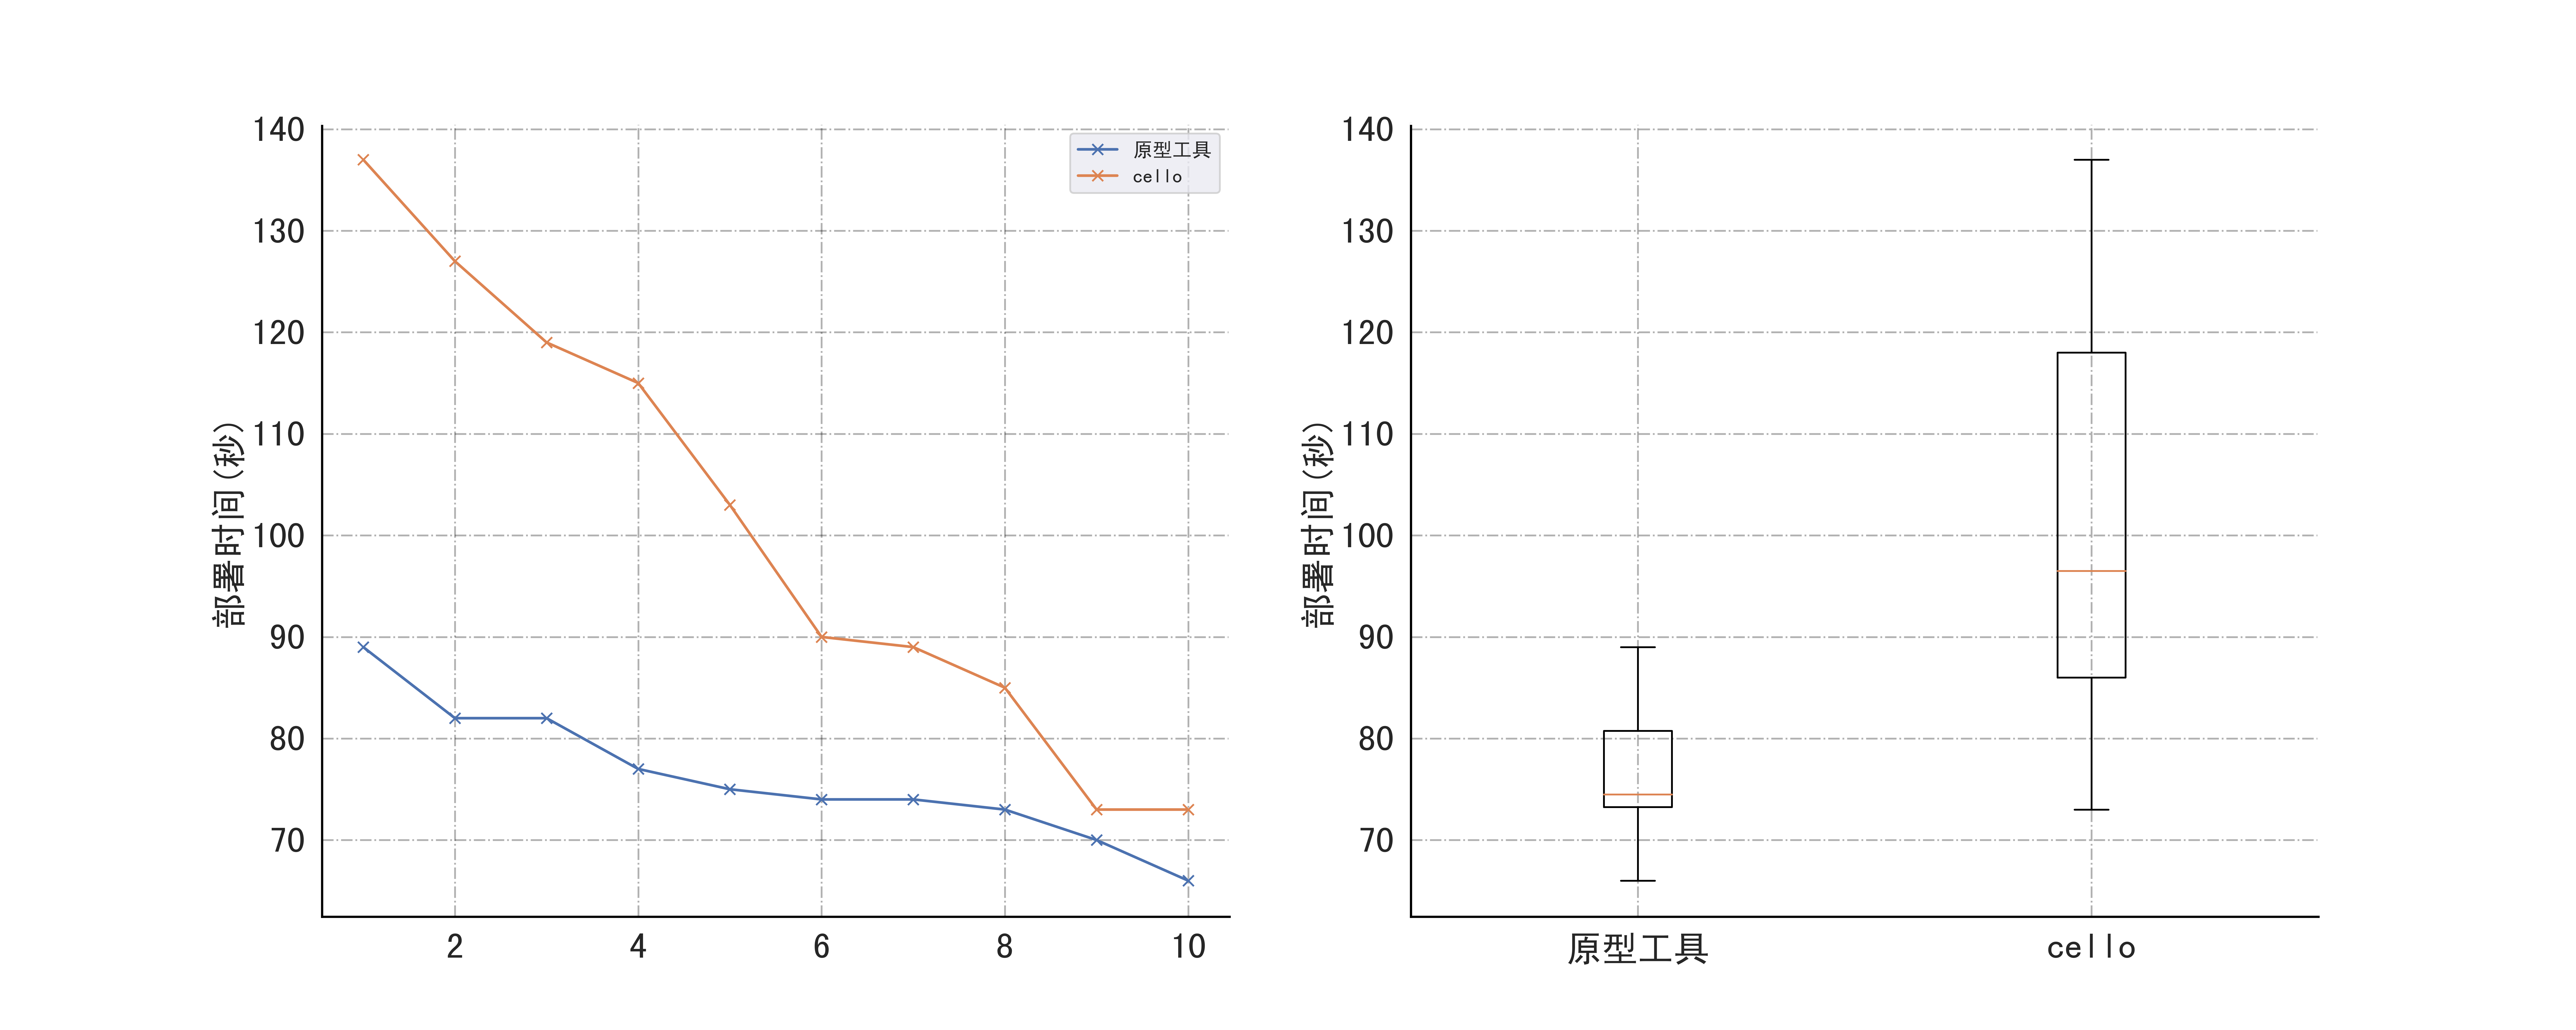
\includegraphics[width=1.0\textwidth]{FIGs/chapter6/plt_deployment.png} %中括号中的参数是设置图片充满文档的大小,你也可以使用小数来缩小图片的尺寸。
    \caption{网络部署时间对比图} %caption是用来给图片加上图题的
    \label{plt_deployment} %这是添加标签,方便在文章中引用图片。
\end{figure}%figure环境

如图\ref{plt_deployment}展示了原型工具和Cello分别部署HF网络的对比图。值得注意的是, 由于Cello采用图形化界面无法配置单个Ca的启停, 所以采用Cello部署的单Orderer单组织的HF网络仅在单个组织内部启动了一个Ca节点, 共计3个网络节点。 而采用原型工具部署的单Orderer单组织的HF网络分别为Orderer以及单组织部署了一个Ca节点, 共计4个网络节点。图\ref{plt_deployment}左侧展示了10次部署排序后的时间曲线图, 图中可以较为直观的看到原型工具比Cello部署的时间要少, 原型工具部署整体网络的平均时间为76.2秒, 而Cello部署整体网络的平均时间为101.1秒; 经计算, 原型工具的总体标准偏差约为6.29, Cello的总体标准偏差约为21.41。图\ref{plt_deployment}右侧分别展示了两者的箱线图, 结合标准偏差可知原型工具部署时间相对而言更为稳定, 尤其在部署Ca节点时, 稳定在13秒左右。

通过分析源码\footnotemark[1]\footnotetext[1]{\href{https://github.com/hyperledger/cello/blob/release-0.9.0-h3c/src/modules/blockchain_network.py}{cello create network}}可知, 当在Cello Operator前端中提交网络之后, Cello对应的Docker Agent会循环解析传入的HF网络节点信息及数量的数据结构, 解析完成后串行构建HF网络中的各类节点。构建过程中, 生成Docker Compose文件并启动对应的网络节点。同样, 当Cello选择在Kubernetes部署时根据Template模板在代码中硬编码生成Yaml文件。由此可得, Cello网络部署时间会随着HF网络中节点数量的增加而线性递增。本文的原型工具, 因需要手动以命令方式部署对应的网络节点, 其部署时间也会随着节点数量增加而递增。因此, 只对单Orderer单Peer进行对比测试即可预估出不同网络规模下的网络部署时间。

在链码部署方面, Cello与原型工具都需要经过创建通道、将账本节点加入至通道内、安装链码等过程。在Cello中上述过程均在图行化界面中配置完成, 原型工具通过命令行方式构建。这两者在安装链码这个环节均在1s内完成, 这对于HF开发人员而言都是能够接受的, 所以这两者仅在安装链码这个环节不需要进行对比。智能合约微服务化的优势在于将智能合约进行解耦, 将智能合约单独作为可交付物。同时开发人员可以利用传统成熟的工具链扩充智能合约开发运维领域的工具空白, 利用已有成熟工具对智能合约进行持续测试、持续交付与持续监控。

{\footnotesize
\begin{longtable}[h]{m{35pt}|m{15pt} m{15pt} m{15pt} m{15pt} m{15pt} m{15pt} m{15pt} m{15pt} m{15pt} m{15pt}|m{20pt}}
    \caption[链码交付时间(单位: 秒(s))]{链码交付时间(单位: 秒(s))} \label{cc_deployment_time}\\
        \hline
        \multirow{2}*{工具类型}
        & \multicolumn{10}{c|}{序号}
        & \multirow{2}*{\parbox[c]{20pt}{平均}}\\
        \cline{2-11}
        & 1 & 2 & 3 & 4 & 5 & 6 & 7 & 8 & 9 & 10 & \\
        \hline
        Cello  & 141 & 128 & 185 & 153 & 166 & 105 & 137 & 160 & 186 & 117 & 147.7\\
        \hline  
        \multirow{1}*{\parbox[c]{40pt}{原型工具}}
        & 119 & 89 & 100 & 76 & 104 & 140 & 136 & 125 & 83 & 164 &  113.6 \\
        \hline
    \end{longtable} 
}

本文对比链码部署过程中所有消耗的时间, 即HF开发人员编写完链码后到将链码成功部署于HF网络节点上所用的时间。如表\ref{cc_deployment_time}展示了原型工具和Cello分别部署asset链码所用的时间对比表。Cello部署链码依次为: 创建通道、加入节点、代码仓库下载链码、压缩链码、计算压缩包MD5、上传链码、安装链码; 原型工具在持续交付流水线中的流程为: 创建通道、加入节点、代码仓库下载链码、打包链码镜像、安装链码。值得注意的是, 本次由于人工操作以及网络波动等情况, 数据可能会存在偏差。最终, Cello的部署链码的平均时间为147.7秒, 原型工具部署链码的平均时间为113.6秒。

综上, 本节对Cello与原型工具进行了定量的对比分析。在网络节点部署方面, 本文原型工具相较于Cello在具有更优的节点部署时间, 并且每次节点部署时间更加稳定。虽然在链码的部署时间方面原型工具表现的较为良好, 但智能合约微服务化的开发运维流程相较于Cello固定式的部署流程能够在流水线中纳入更多的环节如智能合约代码质量、安全等, 以促进智能合约更全面的发展。

\section{本章小结}

本章介绍了对原型工具的测试与评估。首先介绍了本文涉及到的两个测试环境, 并进行了三个维度的评估工作: (1)基本能力自证, 利用典型案例研究的方式进行功能可行性测试, 利用SAAM架构评估方式进行质量属性验证; (2)成熟度衡量, 利用五层成熟度模型的定性评估;(3)对比分析, 与Cello对比的定量分析。


\chapter{总结与展望}

\section{总结}

区块链网络具有去中心化、不可伪造、不可篡改的特性, 其被称为下一代的新型生产关系。随着区块链概念的普及, 其为供应链、金融等传统领域带来了巨大变革。当前, 去中心化应用逐步从概念验证阶段转变为工程化实践阶段。在去中心化应用落地的过程中, 在区块链网络的构建上消耗了大量的时间成本。BaaS基于包括云容器集群在内的云原生技术体系可以帮助区块链开发人员构建、管理、托管区块链网络, 这降低了去中心化应用的落地门槛。

然而, 当前BaaS平台依旧存在着诸多挑战。首先是商业化应用工具不完善, 当前BaaS平台由云提供商巨头把控, 行业马太效应明显。不同云厂商拥有其独立的BaaS平台, 缺乏顶层规划导致多云网络及区块链数据孤岛。其次, 虽然各个云厂商拥有独立的BaaS平台及其相关生态, 但本质上还是将云原生平台作为部署环境, 仅提供一种类似于脚本化部署区块链网路的功能, 远未挖掘云原生底层弹性伸缩、安全性等特性。

因此, 本文针对上述存在的挑战, 本文提出了一种面向Hyperledger Fabric的区块链云化框架。由于Kubernetes Operator可以将领域知识有效的集成到云原生基础设施, 充分发挥云原生的特性。因此本文首先对Kubernetes Operator进行快速评审, 快速评审的范围涵盖了计算机与软件工程领域的4个权威全文数据库并将Scoups和谷歌学术作为补充。将得到的51篇论文经过筛选得到15篇, 对这15篇论文进行数据抽取获得了基于Kubernetes Operator云化的策略集。针对策略集中的策略在区块链背景中进行适配获得了具体区块链云化的具体实施方案。

其次, 根据区块链云化的具体实施方案设计实现了面向Hyperledger Fabric的区块链云化框架及其原型平台。云化框架及其原型平台利用Operator将分别管理HF网络中的Ca、Orderer、Oeer节点。CRD作为框架的输入, 根据官方功能以及配置对节点的属性进行可插拔配置, 如Ca节点的CRLSizeLimit、Orderer节点的Genesis、Peer节点的LevelDB/CouchDB; Manager作为中枢处理单元, 通过对应三个Controller对上述三个节点进行协调循环, 时刻保持节点状态在期望状态。同时, 本文结合实施方案中的策略来提升框架及HF网络的的可迁移性、数据可扩展性、安全性以及可视运维的能力并支持通过命令行方式启停HF网络节点; HF网络作为输出, 包含维持HF网络节点稳定运行的Deployement、Service等Kubernetes配置。

最后, 本文对原型工具进行了全面的测试与评估。以典型案例的方式搭建了单Orderer单组织的HF网络进行功能性测试, 并能够利用云原生的特性满足工具的易用性、可扩展性、安全性等非功能性需求; 在框架及原型工具的评估方面, 本文不仅采用定性分析的方式结合五层成熟度模型对原型工具进行评估而且采用定量分析的方式对比HF官方BaaS平台Cello在网络部署时间上进行了全面对比。结果表明, 原型工具基本满足五层成熟度模型的功能且在部署时间和时间稳定性上优于Cello。


本文提出的面向Hyperledger Fabric的区块链云化框架及其原型工具依托于Kubernetes基础设施, 可以方便的迁移到支持Kubernetes的任何云, 包括公有云、专有云以及混合云, 打破云厂商的垄断格局; 利用输入本应由领域专家执行的参数与操作, 减轻HF网络管理员的负担。利用Kubernetes Operator更原生的管理HF网络, 复用Kubernertes API的公共功能, 如PVC存储、资源隔离、内置认证等方式更好的发挥云原生的潜能, 提升HF网络的易用性、可迁移性、数据可扩展性、安全性以及可视运维的能力。

\section{局限}

本文搭建了原型平台并与Cello进行对比验证, 虽然原型平台在网络部署时间上优于Cello, 但本文提出的面向Hyperledger Fabric的区块链云化框架及其原型工具依旧还有很多局限性:

\begin{itemize}[itemindent=2em]
    \item 为轻量级、快速的将已有知识转移到实践中, 在区块链云化框架调研过程中采用了快速评审的方式, 其相对于系统文献综述(Systematic literature reviews, 简称SLRs)而言缺乏更加深层次的知识掌握。同时Kubernetes Operator以及云原生技术体系在工业界应用广泛而本文的快速评审面对的对象重点是学术工作, 未对灰色文献进行调研。

    \item 本文的Manager中枢控制系统利用Controller对Helm进行进行生命周期监控, 并通过CRD的配置对Helm value进行参数传递。这种方式虽然有利于快速启动Fabric网络, 但增加了Helm作为中间传递的过程, 未能直接对HF网络节点本身的Deployment等配置进行关联。同时, 由于Kubernetes版本的升级所限, 在Helm chart中配置的apiVersion均需要支持Kubernetes 1.18版本及其以上。

    \item 在框架评估方面, 虽然基本满足五层成熟度模型的能力要求, 但目前原型工具尚未具备数据备份和恢复的能力, 未对当前原型工具及所搭建的区块数据进行远端备份。在可伸缩及可扩展性方面, Kubernetes Operator云化策略集中包含支持HPA、VPA的的可伸缩处理, 由于区块链本身的特性, 本文未对Peer进行HPA。但区块链云化框架原则上可以支持Peer的VPA, 并且针对Orderer节点, 区块链云化框架未提供任何可伸缩的处理方式。

    \item 本文的虽然与Cello进行了验证评估工作, 但目前仅针对于网络部署时间这一方面, 而且目前仅对Docker环境进行对比分析, 受到环境所限, 未能使用Cello在Kubernetes中进行部署对比。Cello部署的Hyperledger Fabric为1.4版本, 原型工具部署的版本为2.X版本, 在版本上有些许不同。

    \item 本文在测试评估阶段选取了官方链码asset进行案例研究, 但这并非企业的完整大型应用, 缺乏在大规模HF网络测试评估。并且, 虽然原型工具能够通过命令行的方式进行HF网络及其链码的搭建, 这虽然对于软件工程师而言门槛较低, 但仍未提供图形化的方式。

\end{itemize}



\section{展望}

本文提出的面向Hyperledger Fabric的区块链云化框架及其原型工具能够有效的利用Kubernetes Operator对HF网络进行云化, 但依旧存在不足, 本文仍需在以下发面进行进一步优化提升。

\begin{itemize}[itemindent=2em]
    \item 深入调研学术界以及工业界关于Kubernetes Operator赋能其他领域提升质量属性的策略, 尤其增加对于灰色文献的调研并对本文的策略集进行补充, 最终应用到区块链云化框架及其原型工具中。

    \item 依托于本文的原型工具, 进一步抽象封装提供图形化界面支持; 同时, 结合可扩展性策略, 对HF网络的Peer增加VPA配置, 对Orderer节点增加HPA以及VPA配置, 使其具备弹性伸缩的能力提供更加稳定的服务; 进一步研究针对不同账本存储单元的扩充, 并提供将原型工具和区块账本数据远程备份的策略, 增强数据备份与恢复机制; 有效利用Prometheus监控体系抓取出来的监控指标数据, 进一步挖掘数据深层次的价值。 

    \item 进一步增加对框架及原型工具的评估手段, 面向企业级大规模区块链业务场景, 整理更多专家及HF开发人员对框架及其原型工具的评价, 并不断汲取、筛选适合区块链场景的云化策略进行不断升级改造。 

\end{itemize}


% \chapter{论文引用}

\section{引文相关}
此处的论文引用采用的是类似于IEEE的按出现位置的数字编号格式。建议将被引用的论文全名放入dblp网站(必应谷歌搜索dblp)搜索,之后进入该论文详细信息,如图~\ref{fig_dblpForBibtexCH7} 所示。

\begin{figure}[htb]
  \centering
  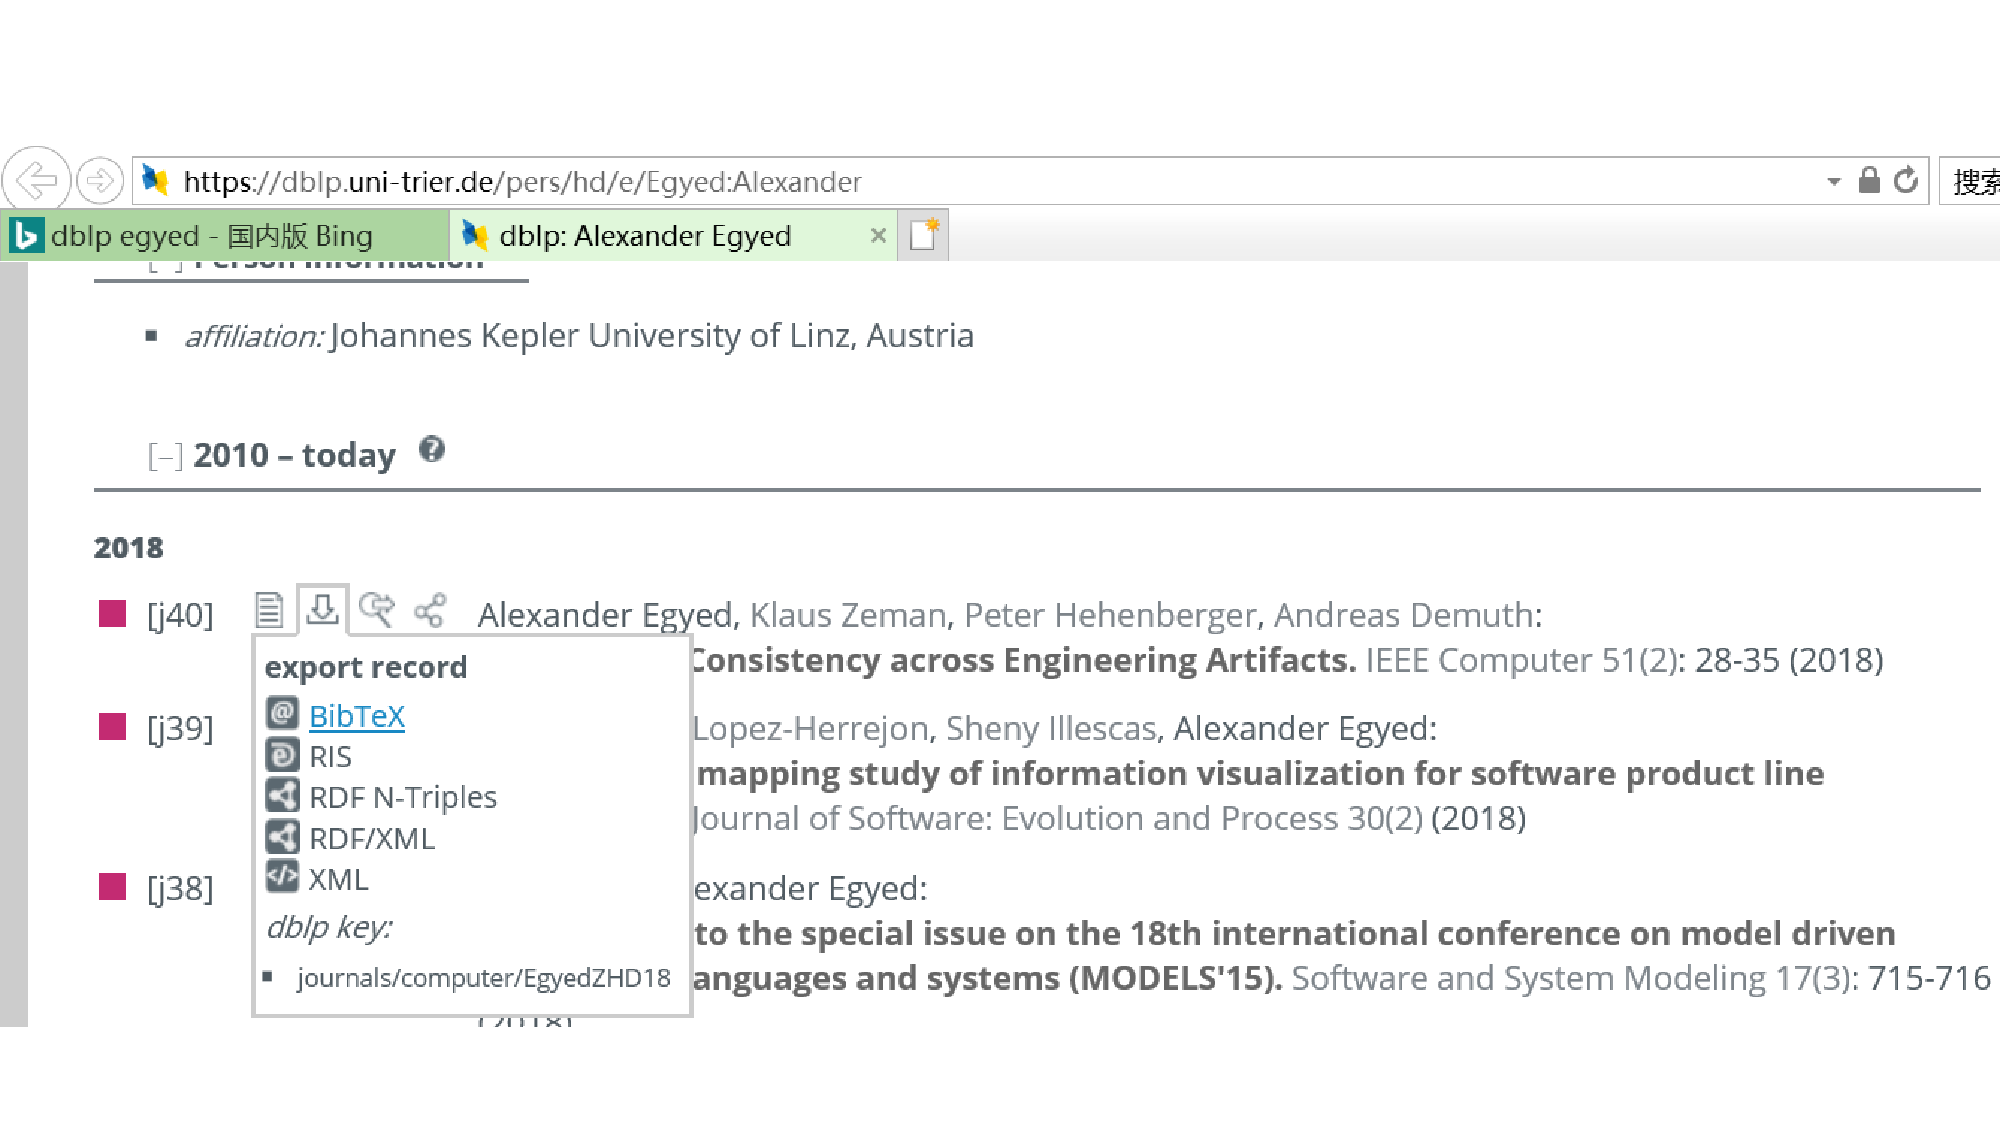
\includegraphics[width=5in]{FIGs/chapter7/dblpForBibtex.pdf}
  \caption{在dblp上下载Bibtex}\label{fig_dblpForBibtexCH7}
\end{figure}

点击该链接之后将得到Bibtex信息,如图~\ref{fig_bibtexDetailCH7}所示。
打开本地文件夹下的reference.bib文件,完整添加该信息。
并在需要引用的位置添加这一引用~\cite{DBLP:journals/computer/EgyedZHD18}。
格式为bibtex信息中的开头,\emph{例如图中的“DBLP:journals/computer/EgyedZHD18”。(此处是一个典型的因为长字符串导致的bad box,请参考上述章节的内容手动完整软换行)}。

\textbf{注意:在修改并保存reference.bib文件后,先点击PDFLaTeX旁边的B按钮编译bib文件,之后需要连续使用PDFLaTeX编译两次,直到最后控制台输出的Warnings不再增加,此时才完成一次论文引用的更新。}

在bib文件中出现,但并未在论文中被引用的论文不会出现在最后的参考文献中。如果dblp中并未包含你需要的论文,则可以尝试谷歌或百度学术的搜索结果,一般也包含bibtex信息,但可能不完整或不规范。

引用网站链接可以考虑这一格式~\cite{GanttSystem}(不推荐,网站链接使用脚注更规范些)。

引用书籍可以考虑这一格式~\cite{Pohl2010Requirements}。

中文文献请参考这一格式~\cite{cyg2006}(引用标记请避免中文,否则容易出现编译错误)。

以下英文引用用来测试引文排序是否按照插入顺序,以及多引文是否合并~\cite{DBLP:journals/computer/EgyedZHD18, DBLP:journals/ml/TingZCZWZ19}

\begin{figure}[htb]
  \centering
  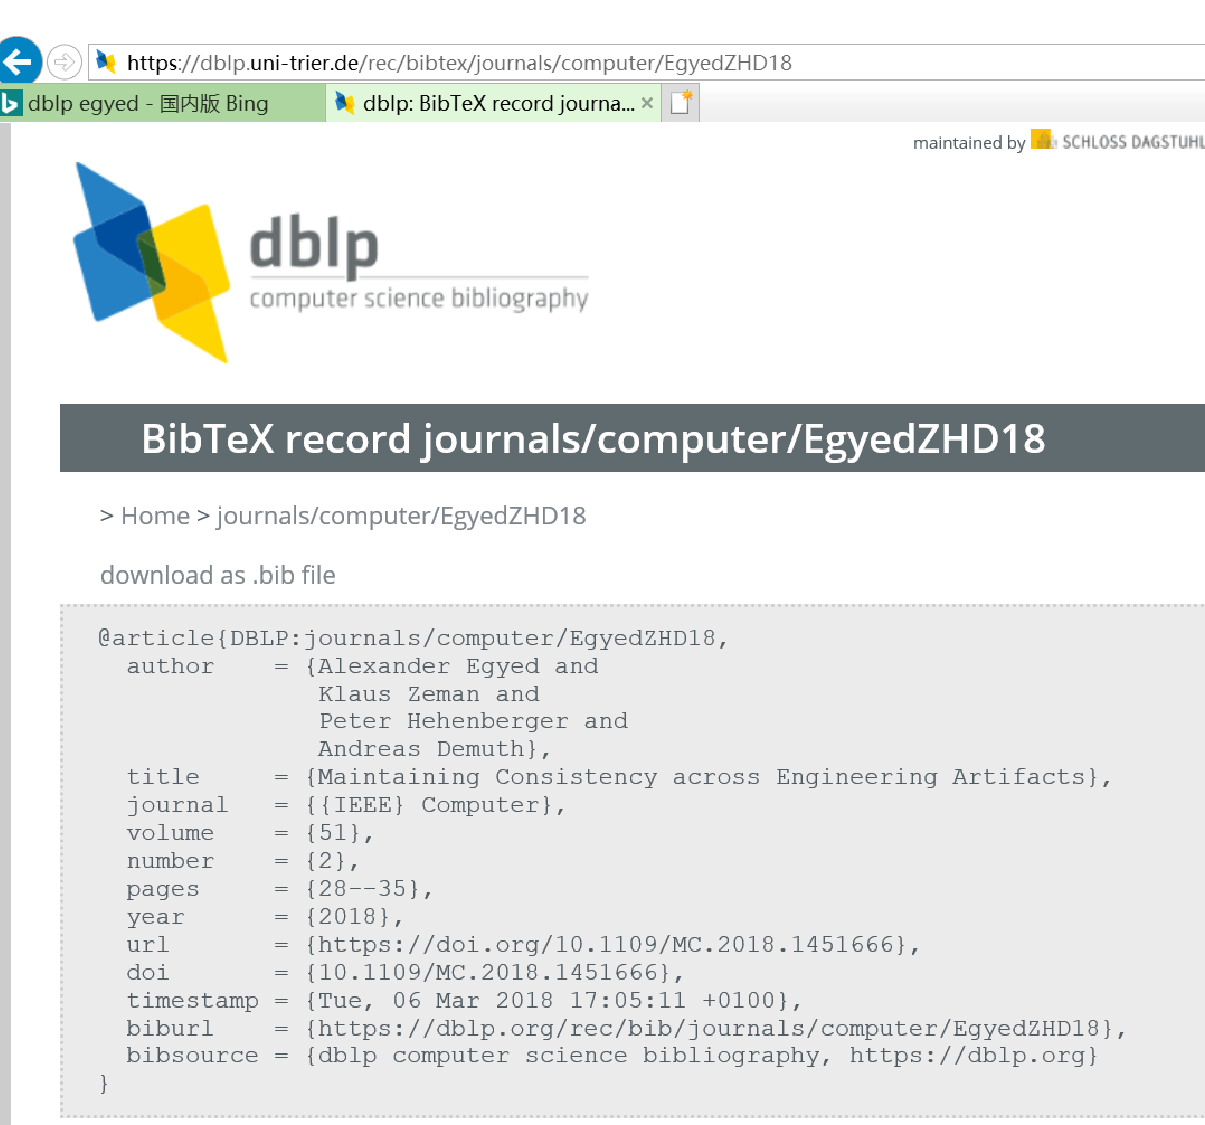
\includegraphics[width=5in]{FIGs/chapter7/bibtexDetail.pdf}
  \caption{Bibtex详细信息}\label{fig_bibtexDetailCH7}
\end{figure}

\section{页眉测试}
以下内容为测试页眉的相关问题、以下内容为测试页眉的相关问题、以下内容为测试页眉的相关问题、以下内容为测试页眉的相关问题、以下内容为测试页眉的相关问题、以下内容为测试页眉的相关问题、

%%%%%%%%%%%%%%%%%%%%%%%%%%%%%%%%%%%%%%%%%%%%%%%%%%%%%%%%%%%%%%%%%%%%%%%%%%%%%%%
% 致谢,应放在结论之后
% \begin{acknowledgement}

% 论文结束之际, 我百感交集。求学路途十九载, 我想真诚感激一路走来帮助我的师长、结伴同行的挚友以及令人难忘的经历, 与你们在结识才铸就了现在的我。

% 在南京大学的三年, 我感谢张贺教授对我的精心指导与帮助。在研究生的三年中, 是我成长的三年、收获的三年。经过张老师的栽培, 我不仅在学术水平上有了显著提升, 更扩宽了我的国际视野, 提升我对理解问题本质的深度与广度。这对我以后的工作生活都受益匪浅。

% 其次, 我要感谢实验室的同门兄弟姐妹们, 感谢你们在研究生三年来对我工作上的指导以及生活上的帮助。忘不了杨岚心师兄在我论文投稿前的字字锱铢, 也忘不掉李杉杉师姐对我完成毕设论文过程中提出的宝贵意见。得益于他们的帮助, 我才能开心顺利地完成我的研究生学业。

% 最后, 更应该感谢一直陪伴着我的父母与家人, 感谢你们背后不辞劳累的支持我, 我很幸运有一个温暖的家。

% 踏出校门, 走进社会。我定会秉承南大“嚼得菜根, 做得大事”的优良品质, 敢于拼搏不畏艰难, 为社会、家人贡献自己的全部。


% \end{acknowledgement}


% 参考文献。应放在\backmatter之前。
% 推荐使用BibTeX,若不使用BibTeX时注释掉下面一句。
%\nocite{*}
\bibliography{sample}


% 附录,必须放在参考文献后,backmatter前
% \appendix
% \chapter{访谈问题}\label{app:1}
% \section{战术建模访谈问题}

%%%%%%%%%%%%%%%%%%%%%%%%%%%%%%%%%%%%%%%%%%%%%%%%%%%%%%%%%%%%%%%%%%%%%%%%%%%%%%%
% 书籍附件
\backmatter
%%%%%%%%%%%%%%%%%%%%%%%%%%%%%%%%%%%%%%%%%%%%%%%%%%%%%%%%%%%%%%%%%%%%%%%%%%%%%%%
% 作者简历与科研成果页,应放在backmatter之后
% \begin{resume}
% % 论文作者身份简介,一句话即可。
%   \begin{authorinfo}
%     \noindent 张富利,男,汉族,1997年8月出生,山东省临沂人。
%   \end{authorinfo}
%   % 论文作者教育经历列表,按日期从近到远排列,不包括将要申请的学位。
%   \begin{education}
%     \item[2015年9月 --- 2019年6月] 中国石油大学(华东)计算机与通信工程学院 \hfill 本科
%   \end{education}
%   % 论文作者在攻读学位期间所发表的文章的列表,按发表日期从近到远排列。
%   \begin{publications}
%       \item \textbf{Fuli Zhang}, Shanshan Li, He Zhang, Hongyu Kuang, Jingyue Li, ``A Blockchain Cloudification Framework for Hyperledger Fabric,'' in Proc. 23rd ACM/IFIP International Middleware Conference(MIDDLEWARE), May. 2022.(Under Review)

%       \item \textbf{张富利},侯培宇,李杉杉,荣国平,李质颖,丁梦洁, ``一种智能合约微服务化框架, '' \textsl{软件学报},2021,32(11):3423-3439.

%       \item Lanxin Yang, He Zhang, \textbf{Fuli Zhang}, Xiaodong Zhang, Guoping Rong, ``An Industrial Experience Report on Retro-inspection,'' in \textsl{Proc. International Conference on Software Engineering, Software Engineering in Practice(ICSE-SEIP)}, May. 2022.

%       \item Guoping Rong, Yifan Zhang, Lanxin Yang, \textbf{Fuli Zhang}, Hongyu Kuang, He Zhang, ``Modeling Review History for Reviewer Recommendation: A Hypergraph Approach,'' in \textsl{Proc. International Conference on Software Engineering(ICSE)}, May. 2022.

%   \end{publications}
 

%   \begin{projects}
%     \item 国家重点研发计划(政府间国际科技创新合作)项目:中挪联合面向供应链的高性能区块链系统支撑平台关键技术研究(2019YFE0105500), 2020-2022, 负责智能合约微服务化开发方法
%     \item 通信软件系统的微服务架构提升, 2019-2020.

%   \end{projects}
% \end{resume}

%%%%%%%%%%%%%%%%%%%%%%%%%%%%%%%%%%%%%%%%%%%%%%%%%%%%%%%%%%%%%%%%%%%%%%%%%%%%%%%
% 生成《学位论文出版授权书》页面,应放在最后一页
%\makelicense

%%%%%%%%%%%%%%%%%%%%%%%%%%%%%%%%%%%%%%%%%%%%%%%%%%%%%%%%%%%%%%%%%%%%%%%%%%%%%%%
\end{document}
